\chapter{Nonlinear Solver}
\label{chap:nln_solver}
As preliminary work, several steps were taken to evaluate the validity of the proposed research.
In order to determine the effects of nonlinear convergence upon the timestep size insensitivity of a solution, the \cobra{} software was modified to enable an iterative global Newton's method.
A metric was developed for the evaluation of the nonlinear convergence of a timestep.
To aid in the development of the nonlinear convergence metric and the nonlinear solver, a novel operator-based scaling has been developed to obtain meaningful convergence thresholds.
The scaling of the nonlinear residual is typically done in an arbitrary fashion; a scaling factor that is intrinsically linked to the physics of interest was developed.
This scaling produces a nondimensionalized residual whose magnitude is relative to the physical sources and sinks on a per equation basis. 
Two temporal convergence test 	problems were developed to show that the nonlinear convergence metric can identify situations where a timestep size insensitive simulation may not satisfy the discrete nonlinear equations.
%--------------------------------------------------------------------------------------------------------------------------------------------------------------------
%--------------------------------------------------------------------------------------------------------------------------------------------------------------------
%--------------------------------------------------------------------------------------------------------------------------------------------------------------------
%--------------------------------------------------------------------------------------------------------------------------------------------------------------------
%--------------------------------------------------------------------------------------------------------------------------------------------------------------------
%--------------------------------------------------------------------------------------------------------------------------------------------------------------------
%--------------------------------------------------------------------------------------------------------------------------------------------------------------------
\section{Nonlinear \cobra{} Implementation}
\label{sect:nln_solver:cobra}  
The first stage of the preliminary work was to modify the \cobra{} software.
As obtained, the \cobra{} software used a single-shot linearization  of the semi-implicit method.
In order to evaluate the subdomain nonlinear refinement algorithm, \cobra{} was converted to include a fully iterative Newton solver based upon a line search globalization strategy.
When it is necessary to distinguish between the single-shot linearization algorithmic implementation of \cobra{} and the iterative nonlinear \cobra{} implementation, the former shall be referred to as the legacy solver and the latter as the nonlinear solver.
As such, the \cobra{} software needed to be modified to be able do the following:

\begin{itemize}
\item{Create a data framework for constructing vector quantities such as $\vec{x}^{k}$ and $\vec{F}$.}
\item{Correctly evaluate $\vec{F}(\vec{x}^{k})$ and $\vec{J}(x^{k})$.}
\item{Implement a globalization strategy for Newton's method.}
\end{itemize}

\cobra{} utilized a single-shot linearization for its solution technique.
As a result of that design decision, memory saving techniques were employed in the construction of the software that precluded more than one Newton step.
In particular, there was the implicit assumption within the software that the first Newton iterate, $\vec{x}^{n+1, 0}$, was the old-time variable $\vec{x}^{n}$.
This design decision required the vetting of all subroutines involved with the evaluation of the components of both the nonlinear residual and its Jacobian.
In addition, the assumption that $\vec{x}^{n+1, k} = \vec{x}^{n}$ produced source code that was inconsistent with an iterative Newton method.
The source code was modified to reflect the intended discretization of the governing conservation laws.
To do this, areas had to be identified where: there were implicit cancellation of terms, the new-time variables were used in place of old-time variables, and the old-time variables were used in place of new-time variables.
Where appropriate, the software was changed to reflect the distinction between old-time and iterate variables and to introduce terms that had been assumed to be equal to zero.

Once the appropriate variables were used for the evaluation of the nonlinear residuals and the Jacobian, a Newton loop was introduced to allow multiple Newton steps.
\alg{alg:nl_cobra} contains the current algorithmic implementation of the nonlinear semi-implicit method.

\begin{algo}[H]
\setlength{\baselineskip}{0.625\baselineskip}
\begin{algorithmic}[1]
\Require $\vec{x}^{0}$ and $t^{0}$
\Set $n = 0$
\Loop \; Transient Loop
    \State $t^{n+1} : = t^{n} + \Delta t$
    \State $k = 0$
    \Define $\vec{x}^{n+1,0}$
	\Calculate $\vec{F}(\vec{x}^{n+1,0})$ and $\vec{J}(\vec{x}^{n+1,0})$
    \Loop \; Newton Loop
		\Calculate $\vec{\delta x} = - \vec{J}^{-1}\cdot\vec{F}$
		$j = 0$		
		\Calculate $\vec{x}^{n+1,k+1,j}$
		\Calculate $\vec{F}(\vec{x}^{n+1,k+1,j})$
		\Loop \; Globalization Loop
			\If{ Globalization loop termination criteria not met}
				\Calculate $\lambda_j$
				\Calculate $\vec{x}^{n+1,k+1,j+1} = \vec{x}^{n+1,k} + \lambda \vec{\delta x}$
				\Calculate $\vec{F}(\vec{x}^{n+1,k+1,j+1})$
				\State $j = j + 1$			
			\Else
				\Calculate $\vec{J}(\vec{x}^{n+1,k+1,j})$
				\Exit Globalization Loop
			\EndIf
		\EndLoop			
		\If{ Newton loop termination criteria met}
			\Exit Newton Loop
		\EndIf
	\EndLoop
	\State $n = n + 1$
\EndLoop
\end{algorithmic}
\caption{Nonlinear \cobra{} algorithm.}
\label{alg:nl_cobra}
\end{algo}

In \alg{alg:nl_cobra}, there are three steps that require discussion.
First is the Newton Loop termination criteria.
There are three Newton loop termination mechanisms, listed below.

\begin{enumerate}
\item{$k > k_{\,\text{MAX}}$}
\item{$||(\vec{S}^{k+1})^{-1}\vec{F}^{k+1}||_{\infty} \leq F_{\text{ABS}}$}
\item{$||(\vec{D}^{k+1})^{-1}\vec{\delta x}^{k}||_{\infty} \leq \delta_{\text{ABS}}$}
\end{enumerate}

Current values for $k_{\,\text{MAX}}$, $F_{\text{ABS}}$ and $\delta_{\text{ABS}}$ are $35$, $1.0$E$-05$, and $1.0$E$-10$, respectively.
The scaling vectors, $\vec{S}$ and $\vec{D}$, will be addressed later.

The second is the globalization loop termination criteria.
The globalization strategy implemented in \cobra{} is a line search algorithm \cite{Dennis1996}.
The two globalization loop termination criteria are:

\begin{enumerate}
\item{$\frac{1}{2}||\vec{F}^{k+1, j}||^{2}_{2} < \frac{1}{2}||\vec{F}^{k}||^{2}_{2} - \alpha ||\vec{F}^{k}||^{2}_{2}$ }
\item{$||\lambda_{j+1} \vec{\delta x}^{k}||_{\infty} < \delta_{\text{abs}}$}
\end{enumerate}

The third point requiring discussion is the calculation of the Newton update vector.
If neither of the loop termination criteria are met, then a step-length parameter, $\lambda_j$, is calculated.
On the first pass through the globalization loop within a given Newton step, a quadratic backtracking model is adopted.
On subsequent passes, a cubic-backtracking model is used.
 
Since vector forms of the nonlinear residual and the independent parameters are used in determining nonlinear convergence and in the globalization algorithm, they needed to be easily manipulated.
A subroutine was written to gather the discrete variables of the independent parameters into a single vector.
Additional source code modifications were necessary to construct and gather the components of the nonlinear residual.

The development of the nonlinear solver within \cobra{} took place under strict quality assurance guidelines.
At every step of the development, the legacy solver was required to maintain the same solution.
This verification was dependent upon a larger number of verification and assessment problems.
The output of the unmodified \cobra{} and the modified \cobra{} software was compared to machine precision.
It was required that either the results of the two simulations be identical or that the reason for the difference be identified and understood.
The \cobra{} software has the ability to repeat a time-step.
As such, it was required that the backup capabilities continued to work while nonlinear solver was being implemented.
Additionally, testing was done to ensure that the ability to restart the software mid-simulation was unaffected.
While adding time to the development cycle, the overhead of the quality assurance procedures ensured that the legacy solver could continue to be used for design purposes.

%--------------------------------------------------------------------------------------------------------------------------------------------------------------------
%--------------------------------------------------------------------------------------------------------------------------------------------------------------------
%--------------------------------------------------------------------------------------------------------------------------------------------------------------------
%--------------------------------------------------------------------------------------------------------------------------------------------------------------------
%--------------------------------------------------------------------------------------------------------------------------------------------------------------------
%--------------------------------------------------------------------------------------------------------------------------------------------------------------------
%--------------------------------------------------------------------------------------------------------------------------------------------------------------------
\section{Operator-Based Scaling}
\label{sect:nln_solver:os}
In order to determine the degree to which a state vector, $\vec{x}$, satisfies \eqref{eqn:conservation_equations}, the use of the nonlinear residual is required.
However, due to the units of the residuals for the different conservation equations, their values can vary by orders of magnitude. 
For a given continuity volume, the nonlinear residual will have six components: four for the conservation of mass and two for the conservation of energy.
For each momentum volume, the three conservation of momentum equations will form the three components of the nonlinear residual.
These residuals have the units of the conserved quantities for their corresponding PDEs; \tab{tab:scaling_units_scales} shows the units for the different conservation equations.

\begin{table}[ht]
\centering
\begin{tabular}{@{}l c r @{}} \toprule
Residual & Units \\
\midrule
Conservation of the \NCG{} Field Mass                  & [ \lbm ] \\
Conservation of the Continuous Liquid Water Field Mass & [ \lbm ] \\
Conservation of the Entrained Liquid Water Field Mass  & [ \lbm ] \\
Conservation of the Water Vapor Field Mass             & [ \lbm ] \\
Conservation of the Gaseous Phase Enthalpy             & [ BTU ]  \\
Conservation of the Liquid Phase Enthalpy              & [ BTU ]  \\
Conservation of the Continuous Liquid Field Momentum   & [ $\frac{ \lbm \text{ft} }{\text{s}}$ ] \\
Conservation of the Entrained Liquid Field Momentum    & [ $\frac{ \lbm \text{ft} }{\text{s}}$ ] \\
Conservation of the Gaseous Phase Momentum             & [ $\frac{ \lbm \text{ft} }{\text{s}}$ ] \\
\bottomrule  
\end{tabular}
\caption{Residuals and their units.}
\label{tab:scaling_units_scales}
\end{table}

Due to the range of magnitudes of these residuals it is important to choose a proper scaling factor to ensure that the convergence of each equation is relative to their magnitude.
A challenge that has been addressed in this work is the development of a method for scaling of these residuals that is based upon the physics of interest during a timestep.
In constructing this scaling factor it was determined that the following characteristics were desirable:

\begin{itemize}
\item{$(S_{i}^{k})^{-1} F^{k}_i \approx 1$ when $\vec{x}^{k}$ is a "poor" solution.}
\item{$(S_{i}^{k})^{-1} F^{k}_i \rightarrow 0$ when phase $i$ disappears.}
\item{$0 \leq \abs{(S_{i}^{k})^{-1} F^{k}_{i}} \leq 1 $ for all values of $\vec{x}^{k}_i$.}
\end{itemize}

The scaling used in this work is an operator-based approach.
The governing PDEs can be viewed as a collection of operators, both linear and nonlinear, acting upon the vector of independent parameters.
The summation of these operators must balance to zero for the nonlinear equation to be satisfied.

To illustrate the scaling procedure, we shall consider the discrete conservation of continuous liquid mass \eqref{eqn:si_mass_liq}.
The residual for \eqref{eqn:si_mass_liq} would be \eqref{eqn:res_mass_liq}.

\begin{equation}
\label{eqn:res_mass_liq}
F_{m,l} = \Delta t \left[ V_c \frac{\left(\alpha_l \rho_l \right)^{n+1} - \left(\alpha_l \rho_l \right)^{n}}{\Delta t} + \sum_{NK}\left( <\alpha^n_l \rho^n_l>^{n}_{d} u^{n+1}_l  \cdot \vec{\bar{A}}\right) + \left[(1-\eta)\Gamma + S \right]^{n+1}\right]
\end{equation}

In this equation there are five physically meaningful quantities: the temporal difference, the mass flowing into  the volume, the mass flowing out of the volume, the mass exchange with the gaseous phase, and the mass exchange with the entrained liquid field.

The scaling chosen for this residual is shown by \eqref{eqn:scaling_factor}.
\begin{equation}
\label{eqn:scaling_factor}
S_{m,l} = \Delta t \left[ V_c \abs{\frac{\left(\alpha_l \rho_l \right)^{n+1} - \left(\alpha_l \rho_l \right)^{n}}{\Delta t}} + \sum_{NK}\abs{\left( <\alpha^n_l \rho^n_l>^{n}_{d} u^{n+1}_l  \cdot \vec{\bar{A}}\right)} + \left[\abs{(1-\eta)\Gamma} + \abs{S} \right]^{n+1}\right]
\end{equation}

This scaling creates a relative measure of the nonlinear residual when compared to the magnitude of the physics involved in the process.
The other mass, energy, and momentum equations each have similarly defined scaling factors for their respective residuals.
For convergence testing in the nonlinear version of \cobra{} and residual evaluation during the legacy mode, the scaled nonlinear residual is used.

The issue of phase transition was considered during this work.
Since \cobra{} does not actually transition the governing equations to those for single-phase flow, there will always be a nonlinear residual for those phases that are approximately absent.
It was determined that the effects of maintaining a depleted phase in the system of equations when solving the nonlinear problem created a unique issue.
The unscaled residuals would be on the order of machine round-off.
The operator based scaling factors for these residuals would also be within orders of magnitude of machine round-off.
This created the situation where the scaled nonlinear residual for the depleted field would be of $\mathcal{O}$(1).
These depleted residuals would dominate the determination of convergence.
To overcome this deficiency it was determined that when a phase or field began to deplete, the scaling factor would be scaled up to create an artificial decrease in the residual to counter the artificial presence of the depleted field.
This scaling is shown by \eqref{eqn:scaling_factor_small}.

\begin{equation}
\label{eqn:scaling_factor_small}
S_k = \max[1.0, \left(C_1 \frac{\alpha_{k,\text{MIN}}}{\alpha_k}\right)^{C_2} ] S_k
\end{equation}

For this work, the constant $C_1$ was set equal to 100, and the exponent $C_2$ was set equal to 10.
This particular phase transition scaling produced the regular operator scaling factor when the volume fraction of a phase is at least two orders of magnitude greater than the minimum volume fraction for that phase.
This drove the scaled residuals for phases that were nominally not present to zero.
The original coding of \cobra{} has a minimum volume fraction of $\alpha_{k,\text{MIN}}$ = 1.0E-6.
For the work performed here, that value was reduced to $\alpha_{k,\text{MIN}}$ = 1.0E-9.

\section{Illustrative Problems}
\label{sect:nln_solver:illustrative}

Two test problems were developed to illustrate the effectiveness of the nonlinear solver and the operator based scaling.

\subsection{Geometry}
\label{subsect:experimental_geometry}
For both of the test problems, the same computational geometry was used;  \fig{fig:exp_geometry} represents the experimental geometry.
Each block represents a single continuity cell with a height of 4 [in].
The total height of the channel is 48 [in].
Each continuity cell has a cross-sectional area of 4 [in$^2$].
The red block at the top of the channel represents a boundary cell where the pressure and enthalpy are specified.
It represents an infinite reservoir filled with a fluid at a specified thermodynamic state.
The red triangle represents a specified flow at the bottom edge of the first continuity cell. 

\begin{figure}[h!t]
\begin{center}
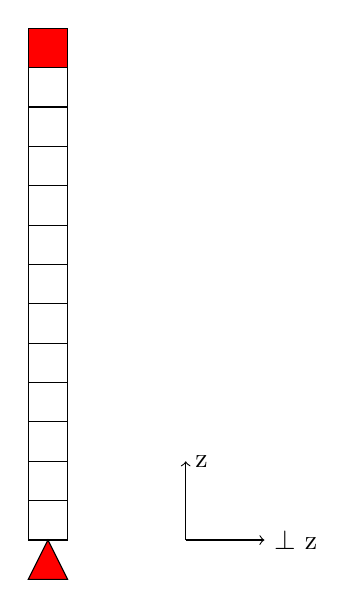
\begin{tikzpicture}
\foreach \x in {1,..., 12} \draw(0, 0.5*\x-0.5) rectangle +(.5,.5);
\filldraw[fill=red] (0, 6) rectangle +(.5,.5); 
\filldraw[fill=red] (0, -0.5) -- (0.25, 0) -- (0.5, -0.5) -- cycle;
\draw[->] (2,0) -- (2, 1) node[anchor=west] {z};
\draw[->] (2,0) -- (3, 0) node[anchor=west] {$\perp$ z};
\end{tikzpicture}
\end{center}
\caption{Geometry for test problems.}
\label{fig:exp_geometry}
\end{figure}

\subsection{Initial and Boundary Conditions}
\label{subsect:ic_bc}

The two problems, while having the same geometry, are different in their dominant physics.
One problem was designed to simulate single-phase, single-field continuous liquid flow in a standpipe.
This problem will be referred to as the single-phase problem.
The second problem was designed such that high-pressure liquid flashes into steam as it enters a standpipe initially filled with saturated vapor at a much lower pressure, known hereafter as the flashing problem.

Table \ref{tab:ic} provides the initial conditions for the two problems.
The pressure, enthalpy, and volume-fractions for the different fields allow for a complete description of the continuity variables.
The initial velocities are set to zero.

\begin{table}[ht]
\centering
\begin{tabular}{@{}lr@{.}lr@{.}lr@{.}lr@{.}lr@{.}l@{}} \toprule
\multirow{2}{*}{Problem} & \multicolumn{2}{c}{Pressure} & \multicolumn{2}{c}{Enthalpy}             & \multicolumn{2}{c}{$\alpha_g$} & \multicolumn{2}{c}{$\alpha_l$} & \multicolumn{2}{c}{$\alpha_e$} \\ 
                         & \multicolumn{2}{c}{[psia]} & \multicolumn{2}{c}{$[\frac{\text{BTU}}{\lbm{}}]$} & \multicolumn{2}{c}{[-]}      & \multicolumn{2}{c}{[-]}      & \multicolumn{2}{c}{[-]}      \\ \midrule
Single-Phase             &  200&0                       &  355&5                                   & 0&0                            & 1&0                            & 0&0 \\
Flashing                 &  200&0                       & 1198&3                                   & 1&0                            & 0&0                            & 0&0 \\ \bottomrule  
\end{tabular}
\caption{Initial conditions for test problems.}
\label{tab:ic}
\end{table}

Each of the problems has a specified pressure-enthalpy boundary condition at the top of the stand pipe and a flow-enthalpy boundary condition at the inlet of the domain.
Table \ref{tab:bc_pe} contains the pressure, enthalpy, and composition of the pressure-enthalpy reservoir. 

\begin{table}[h!t]
\centering
\begin{tabular}{@{}lr@{.}lr@{.}lr@{.}lr@{.}lr@{.}l@{}} \toprule
\multirow{2}{*}{Problem} & \multicolumn{2}{c}{Pressure} & \multicolumn{2}{c}{Enthalpy}             & \multicolumn{2}{c}{$\alpha_g$} & \multicolumn{2}{c}{$\alpha_l$} & \multicolumn{2}{c}{$\alpha_e$} \\ 
                         & \multicolumn{2}{c}{[psia]} & \multicolumn{2}{c}{$[\frac{\text{BTU}}{\lbm{}}]$} & \multicolumn{2}{c}{[-]}      & \multicolumn{2}{c}{[-]}      & \multicolumn{2}{c}{[-]}      \\ \midrule
Single-Phase             &  200&0                       &  355&5                                   & 0&0                            & 1&0                            & 0&0 \\
Flashing                 &  200&0                       & 1198&3                                   & 1&0                            & 0&0                            & 0&0 \\ \bottomrule  
\end{tabular}
\caption{The pressure-enthalpy outlet boundary conditions for test problems.}
\label{tab:bc_pe}
\end{table}

The flow-enthalpy boundary condition describes the thermodynamic state of the inflowing fluid and its flow rate.
Table \ref{tab:bc_fe} describes the inlet boundary condition for the two problems.

\begin{table}[ht]
\centering
\begin{tabular}{@{}lr@{.}lr@{.}lr@{.}lr@{.}lr@{.}l@{}} \toprule
\multirow{2}{*}{Problem} & \multicolumn{2}{c}{Pressure} & \multicolumn{2}{c}{Enthalpy}             & \multicolumn{2}{c}{$\alpha_g$} & \multicolumn{2}{c}{$\alpha_l$} & \multicolumn{2}{c}{$\alpha_e$} \\ 
                         & \multicolumn{2}{c}{[psia]} & \multicolumn{2}{c}{$[\frac{\text{BTU}}{\lbm{}}]$} & \multicolumn{2}{c}{[-]}      & \multicolumn{2}{c}{[-]}      & \multicolumn{2}{c}{[-]}      \\ \midrule
Single-Phase             &  200&0                       &  355&5                                   & 0&0                            & 1&0                            & 0&0 \\
Flashing                 & 1000&0                       &  542&6                                   & 1&0                            & 0&0                            & 0&0 \\ \bottomrule  
\end{tabular}
\caption{The flow-enthalpy inlet boundary conditions for test problems.}
\label{tab:bc_fe}
\end{table}

The specified mass flow, $\dot{m}(t)$, at the bottom of the channels is the same for both problems. 
This time-dependent function is given by \eqref{eqn:bc_time_func_single}.

\begin{equation}
\label{eqn:bc_time_func_single}
\dot{m}(t) = \left\{
\begin{array}{cclrcll}
 0.0           & [\frac{ \lbm{} }{\text{s}}] & , &                & t & \leq 1 & [\text{s}] \\
 0.5 ( t - 1)  & [\frac{ \lbm{} }{\text{s}}] & , & 1\; [\text{s}] < & t & \leq 2 & [\text{s}] \\
 0.5           & [\frac{ \lbm{} }{\text{s}}] & , &                & t & > 2    & [\text{s}]
\end{array}\right.
\end{equation}

Both problems adjust their initial pressure distribution to account for hydrostatic head, which is not specified in the input files.
The \cobra{} input files for both problems can be found in \app{app:input_decks}.

\subsection{Procedure}
\label{subsect:procedures}

The two problems were set up so that the maximum allowable timestep was varied.
Each problem was run with the following maximum allowable timesteps: 1 [s], 0.1 [s], 0.01 [s], 0.001 [s], 0.0001 [s], and 0.00001 [s]. 
For the legacy runs, the scaled residuals were evaluated after a single Newton step, $\vec{F}(\vec{x}^{1})$.
For the nonlinear runs, the scaled nonlinear residuals were evaluated at the end of the Newton-loop.
The nonlinear convergence criteria used in the nonlinear solver are described in \sect{sect:nln_solver:cobra}.
The temporal convergence metric was evaluated during post-processing.
In total, there were twenty-four simulations run.
The two different problems were each run at six different maximum timestep sizes on each of the two versions of \cobra{}.

\subsection{Results}
\label{subsect:results}

The results from the simulation runs will now be analyzed to determine the impact of nonlinear convergence upon time-step size sensitivity.
The solutions produced by both solvers will be compared to determine the efficacy of the residual metric in determining the validity of the nonlinear solution.  

Of the twenty-four simulations run, the legacy solver solution of the flashing problem with a \dtmax{} of 1 [s] failed to run to completion.
The timestep limiting procedure outlined in  \sect{sect:algorithmic_concerns} was unable to prevent too large a change in the independent parameters by reducing the timestep.
This caused the problem to try to run below the minimum allowable timestep size, which resulted in the software aborting.
However, the nonlinearly convergent \cobra{} was able to run at a \dtmax{} of 1 [s].
Both versions of \cobra{} are subject to the same limits on change of independent variables.

For the flashing problem, the parameter of interest for temporal convergence testing is $\alpha_g$ at 2 [in] from the inlet of the stand pipe.
\fig{fig:flashing_1em1} shows the gaseous volume fraction 2 [in] from the inlet of the stand pipe as a function of time for a \dtmax{} of 1.0E-1 [s] for both the legacy and the nonlinear solvers.

%\begin{figure}[h!t]
%\centering
%\subfloat[Solution with \dtmax{} = 1.0E-1 {[s]}]{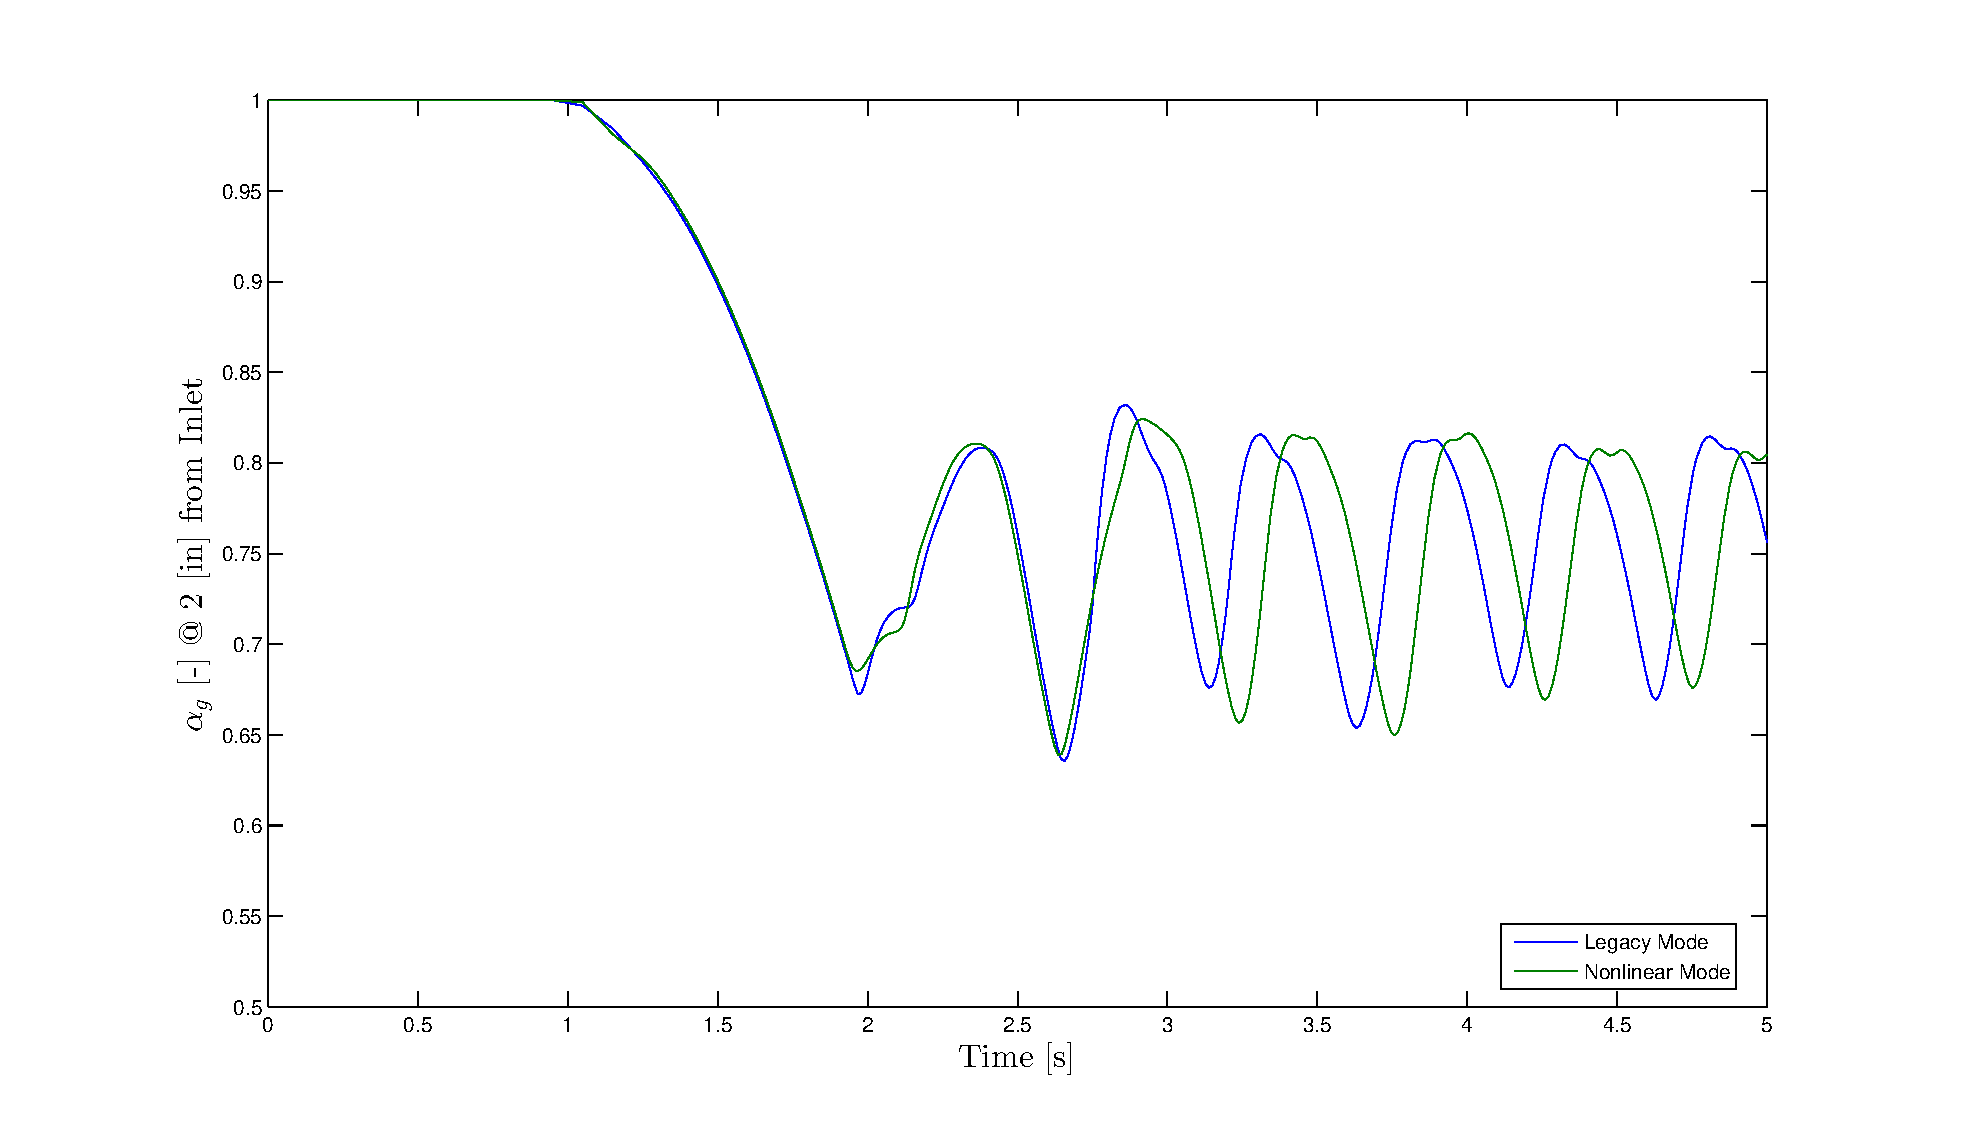
\includegraphics[width=0.49\textwidth]{images/flashing_1em1.eps}
%\label{fig:flashing_1em1}}
%\subfloat[Solution with \dtmax{} = 1.0E-5 {[s]}]{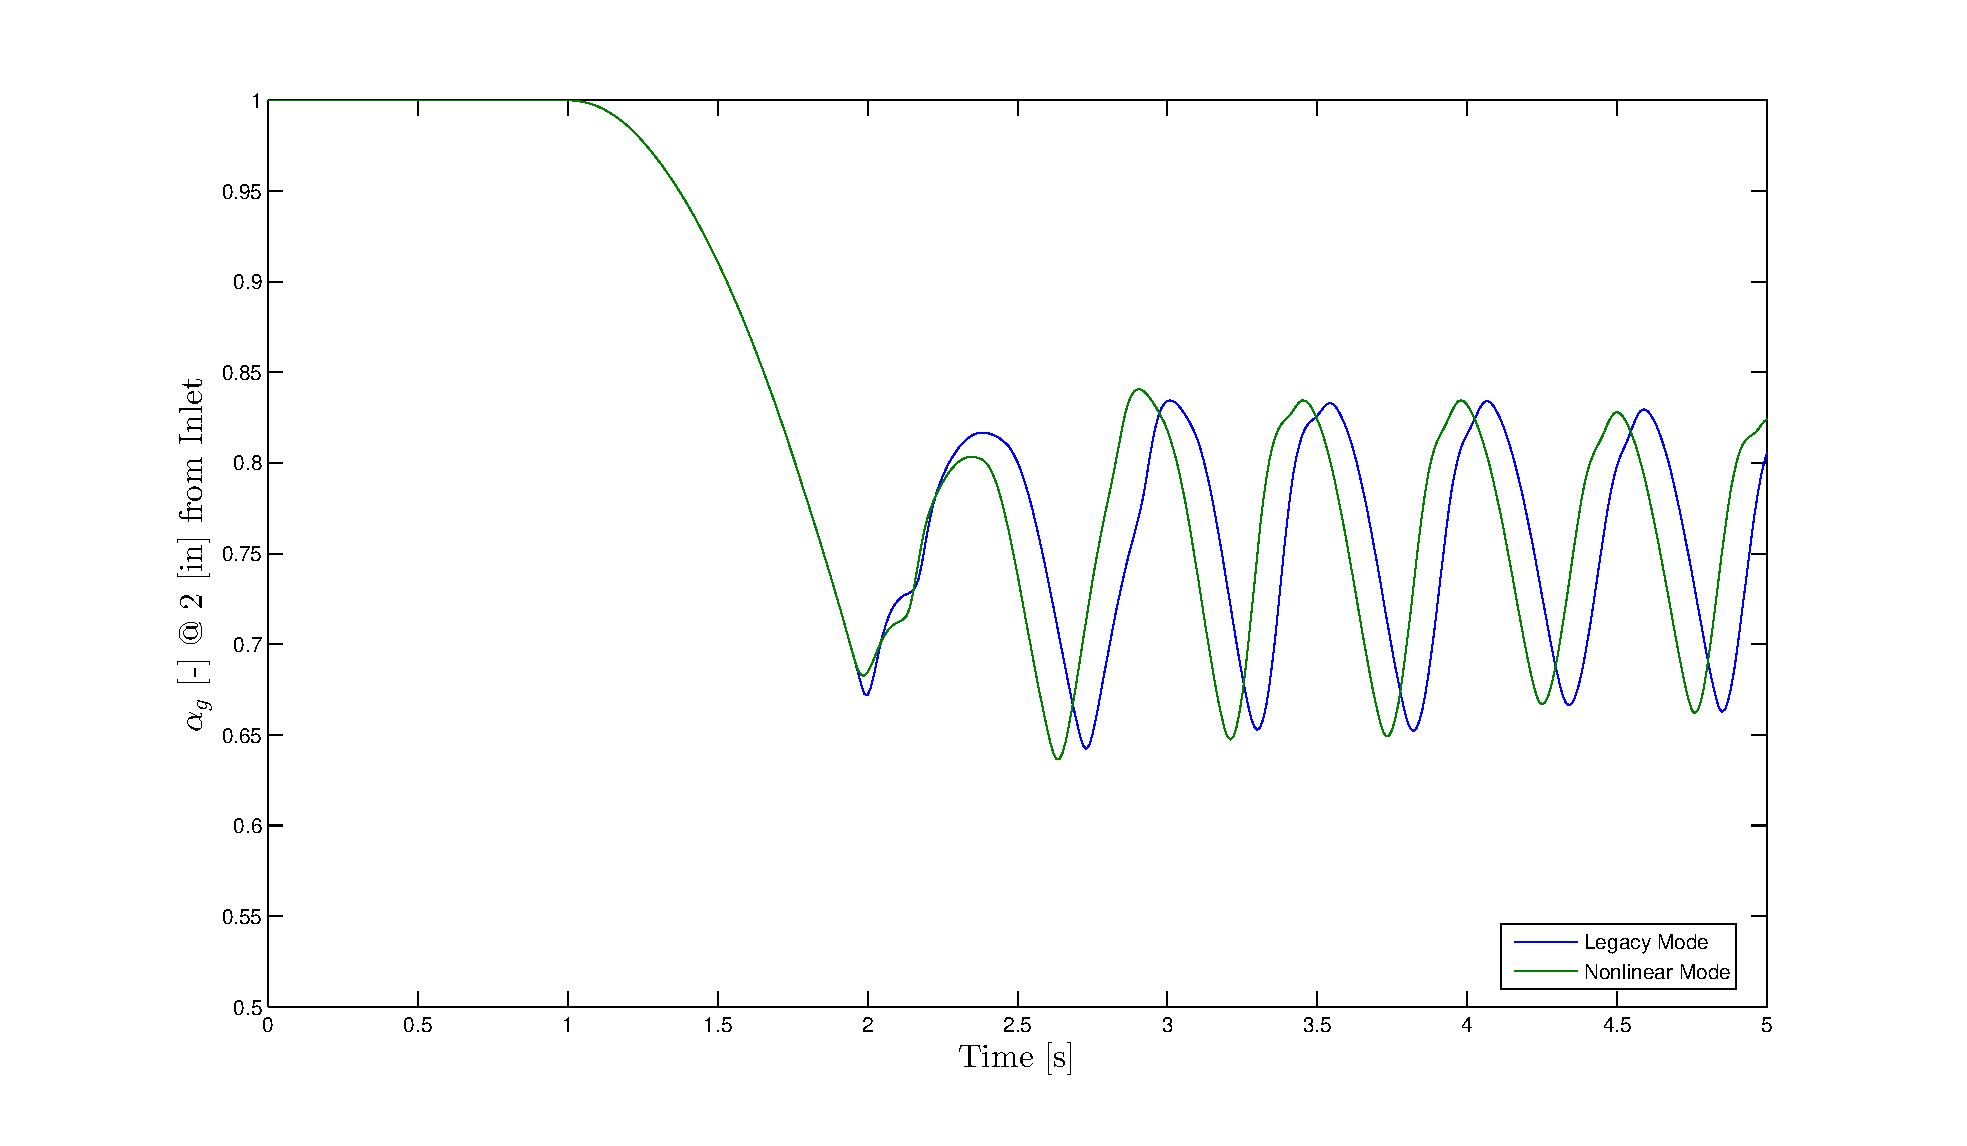
\includegraphics[width=0.49\textwidth]{images/flashing_1em5.eps}
%\label{fig:flashing_1em5}}
%\caption[Flashing solution at \dtmax{} = 1.0E-1 {[s]}and 1.0E-5 {[s]}]{Flashing solution at \dtmax{} = 1.0E-1 {[s]} and 1.0E-5 {[s]}.}
%\label{fig:flashing_compare_1}
%\end{figure}

\begin{figure}[h!t]
\centering
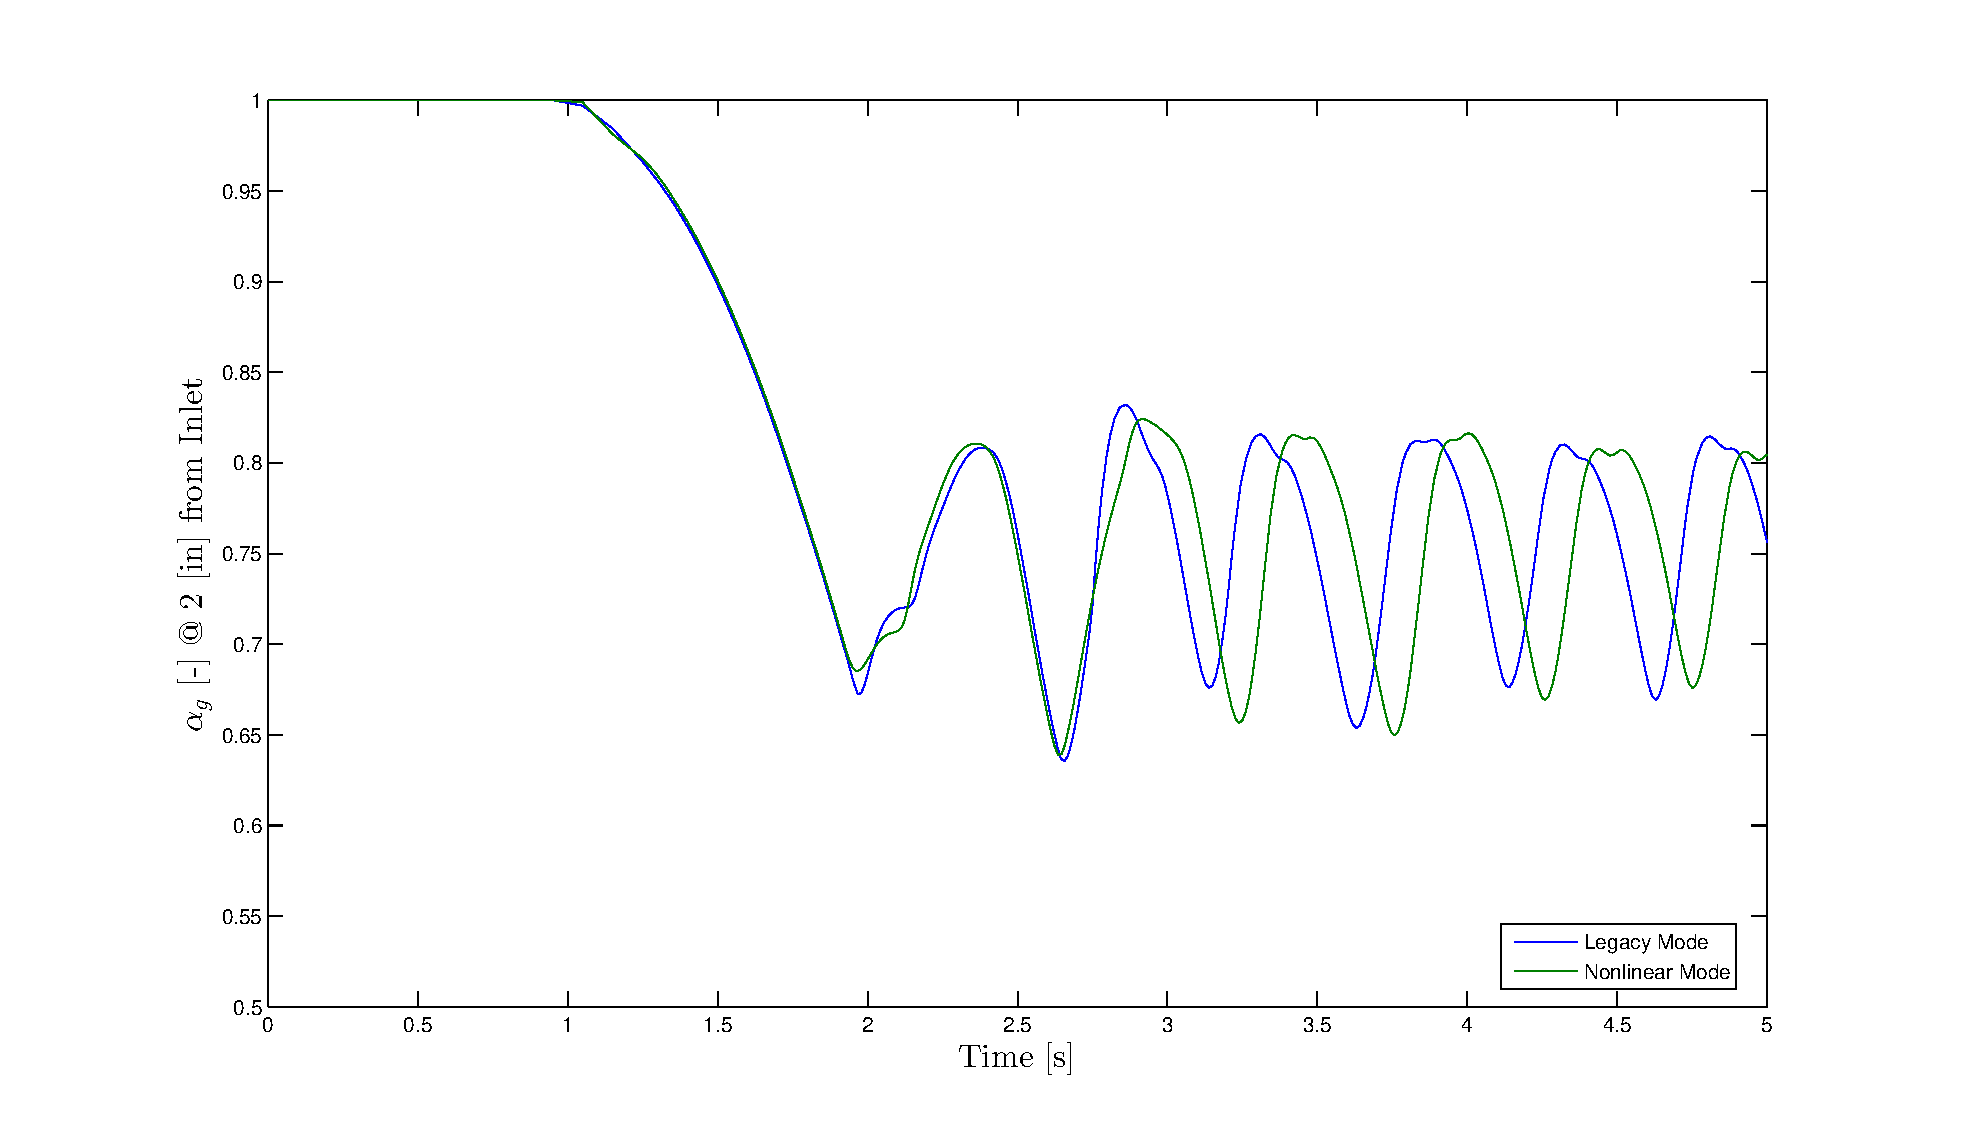
\includegraphics[width=0.94\textwidth]{images/flashing_1em1.eps}
\caption{Flashing solution at \dtmax{} = 1.0E-1 {[s]}}
\label{fig:flashing_1em1}
\end{figure}

\begin{figure}[h!t]
\centering
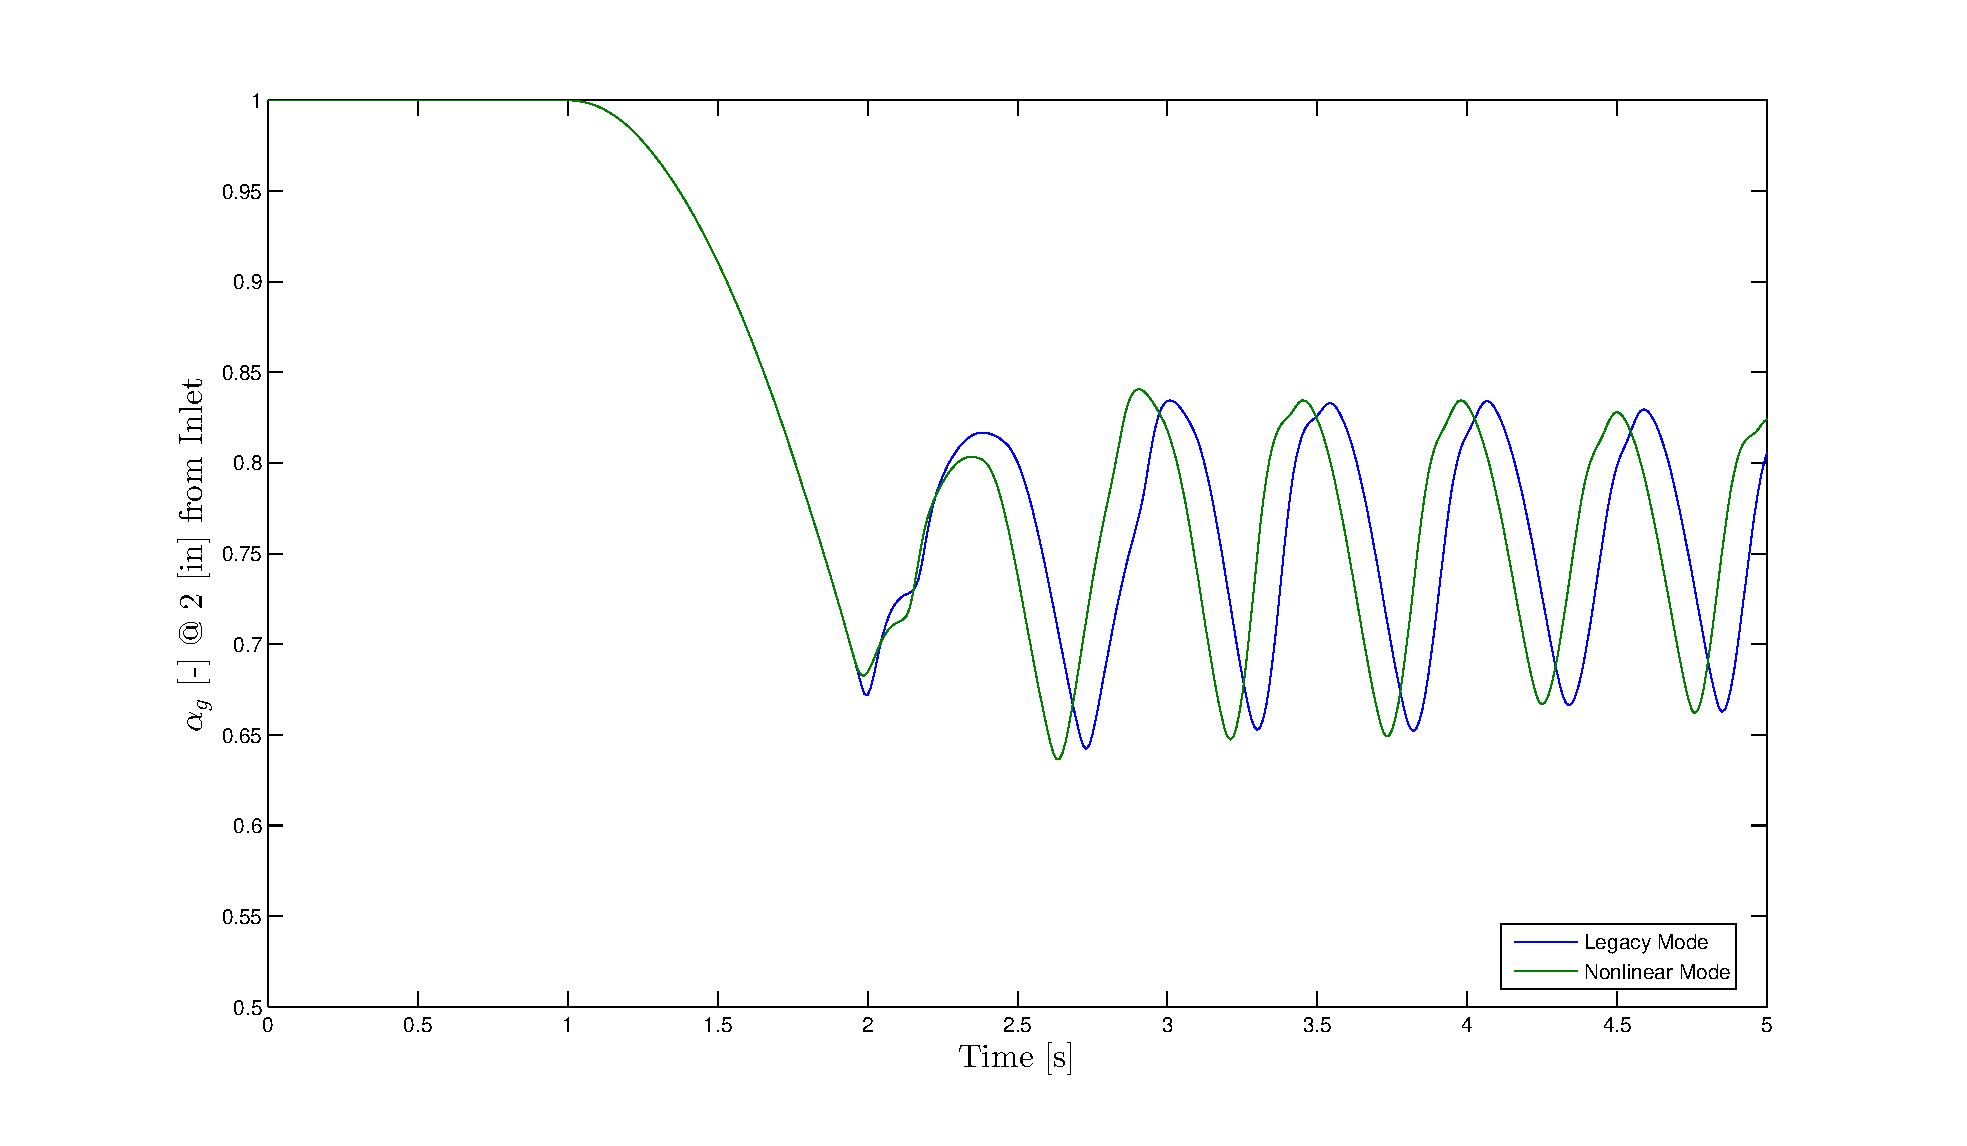
\includegraphics[width=.94\textwidth]{images/flashing_1em5.eps}
\caption{Flashing solution at \dtmax{} = 1.0E-5 {[s]}.}
\label{fig:flashing_1em5}
\end{figure}

Note that the nonlinearly resolved solution is qualitatively different than the legacy single-shot solution, \fig{fig:flashing_1em1}.
Even as the \dtmax{} is reduced, this discrepancy does not disappear, \fig{fig:flashing_1em5}.
The two solutions do not converge to the same solution as the timestep size was reduced.
However, the solution to the flashing problem produced by the nonlinear solver, \fig{fig:nl_mode_flashing}, qualitatively varies less as the timestep size is reduced than that produced by the legacy solver, \fig{fig:cobra_mode_flashing}.
However, both \fig{fig:cobra_mode_flashing} and \fig{fig:nl_mode_flashing} show that as the timestep size is reduced the two different solutions become more timestep size insensitive.

%\begin{figure}[h!t]
%\centering
%\subfloat[Legacy mode solution.]{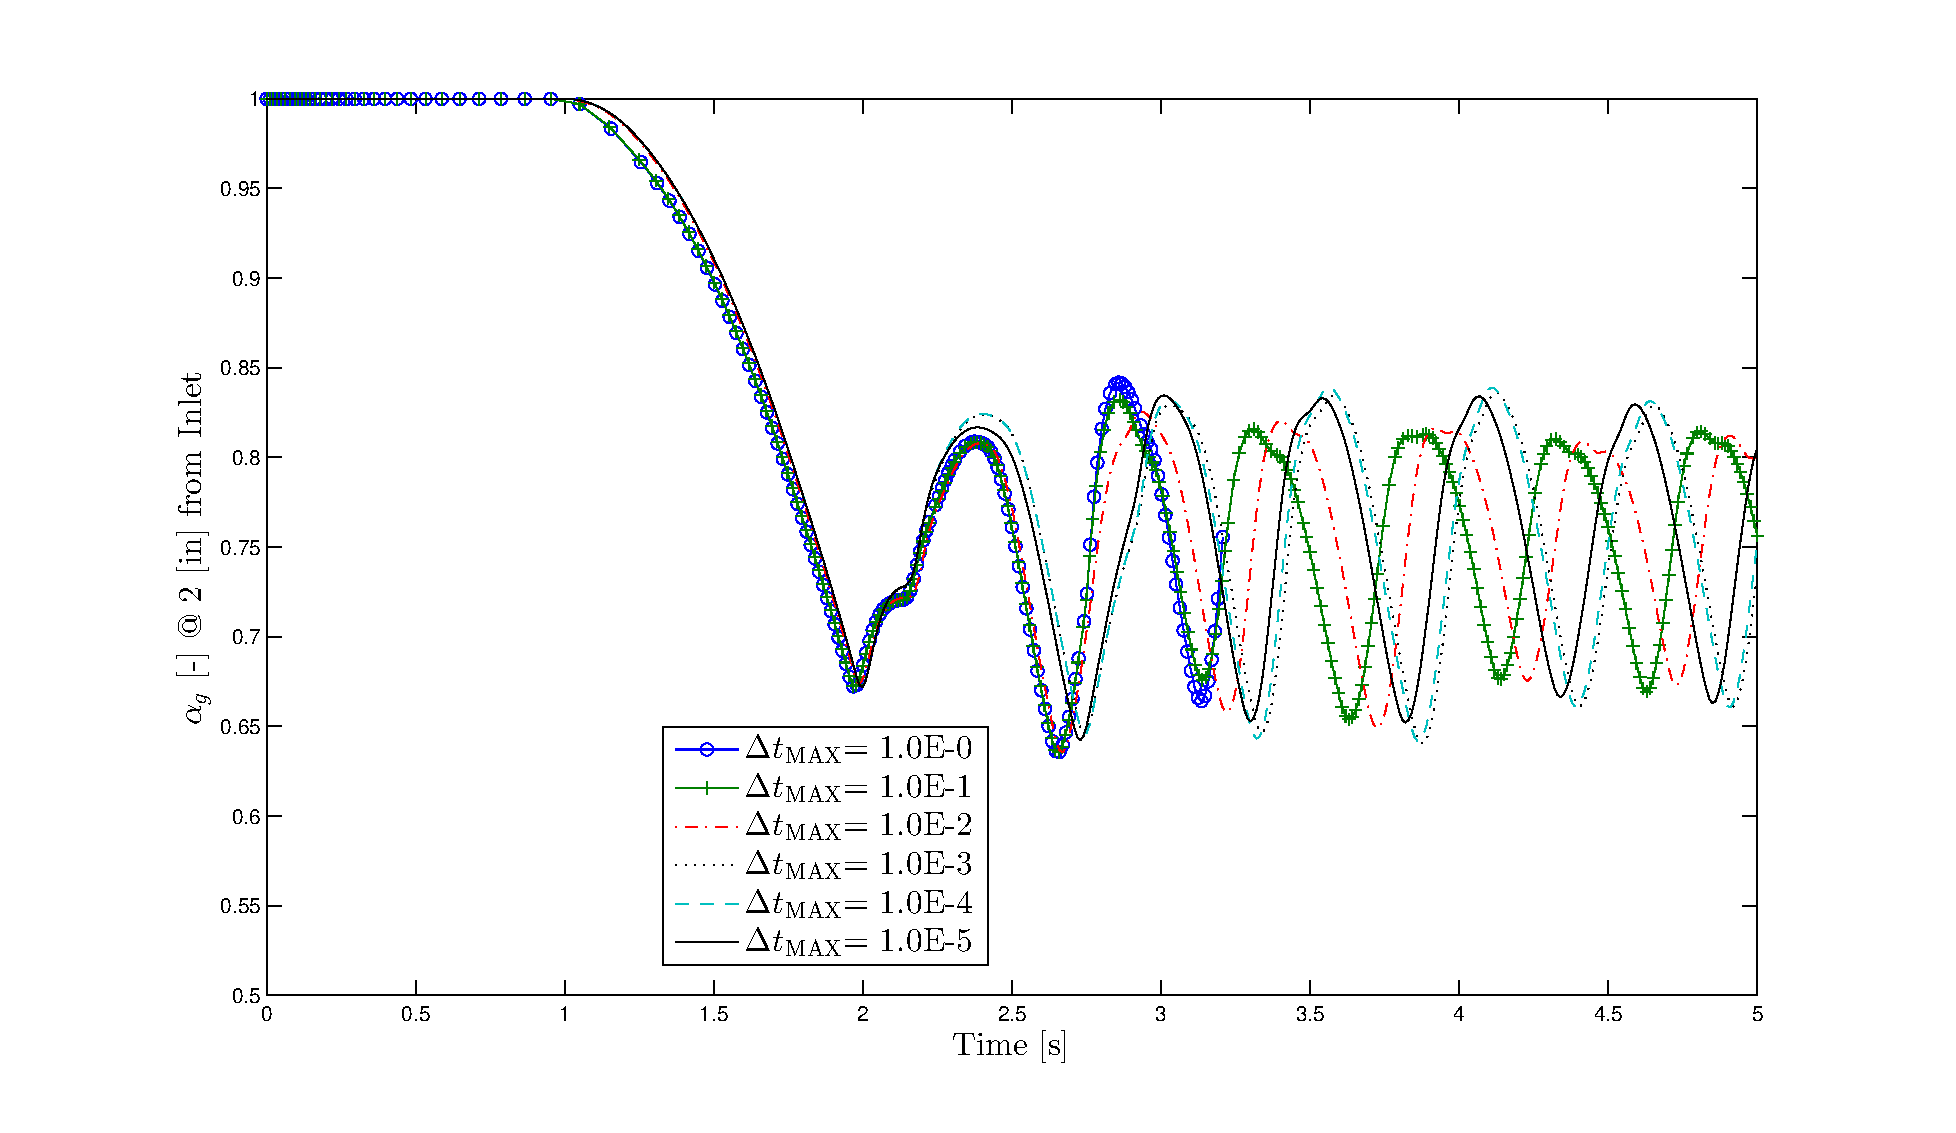
\includegraphics[width=0.49\textwidth]{images/cobra_flashing_al_2in.eps}
%\label{fig:cobra_mode_flashing}}
%\subfloat[Nonlinear mode solution.]{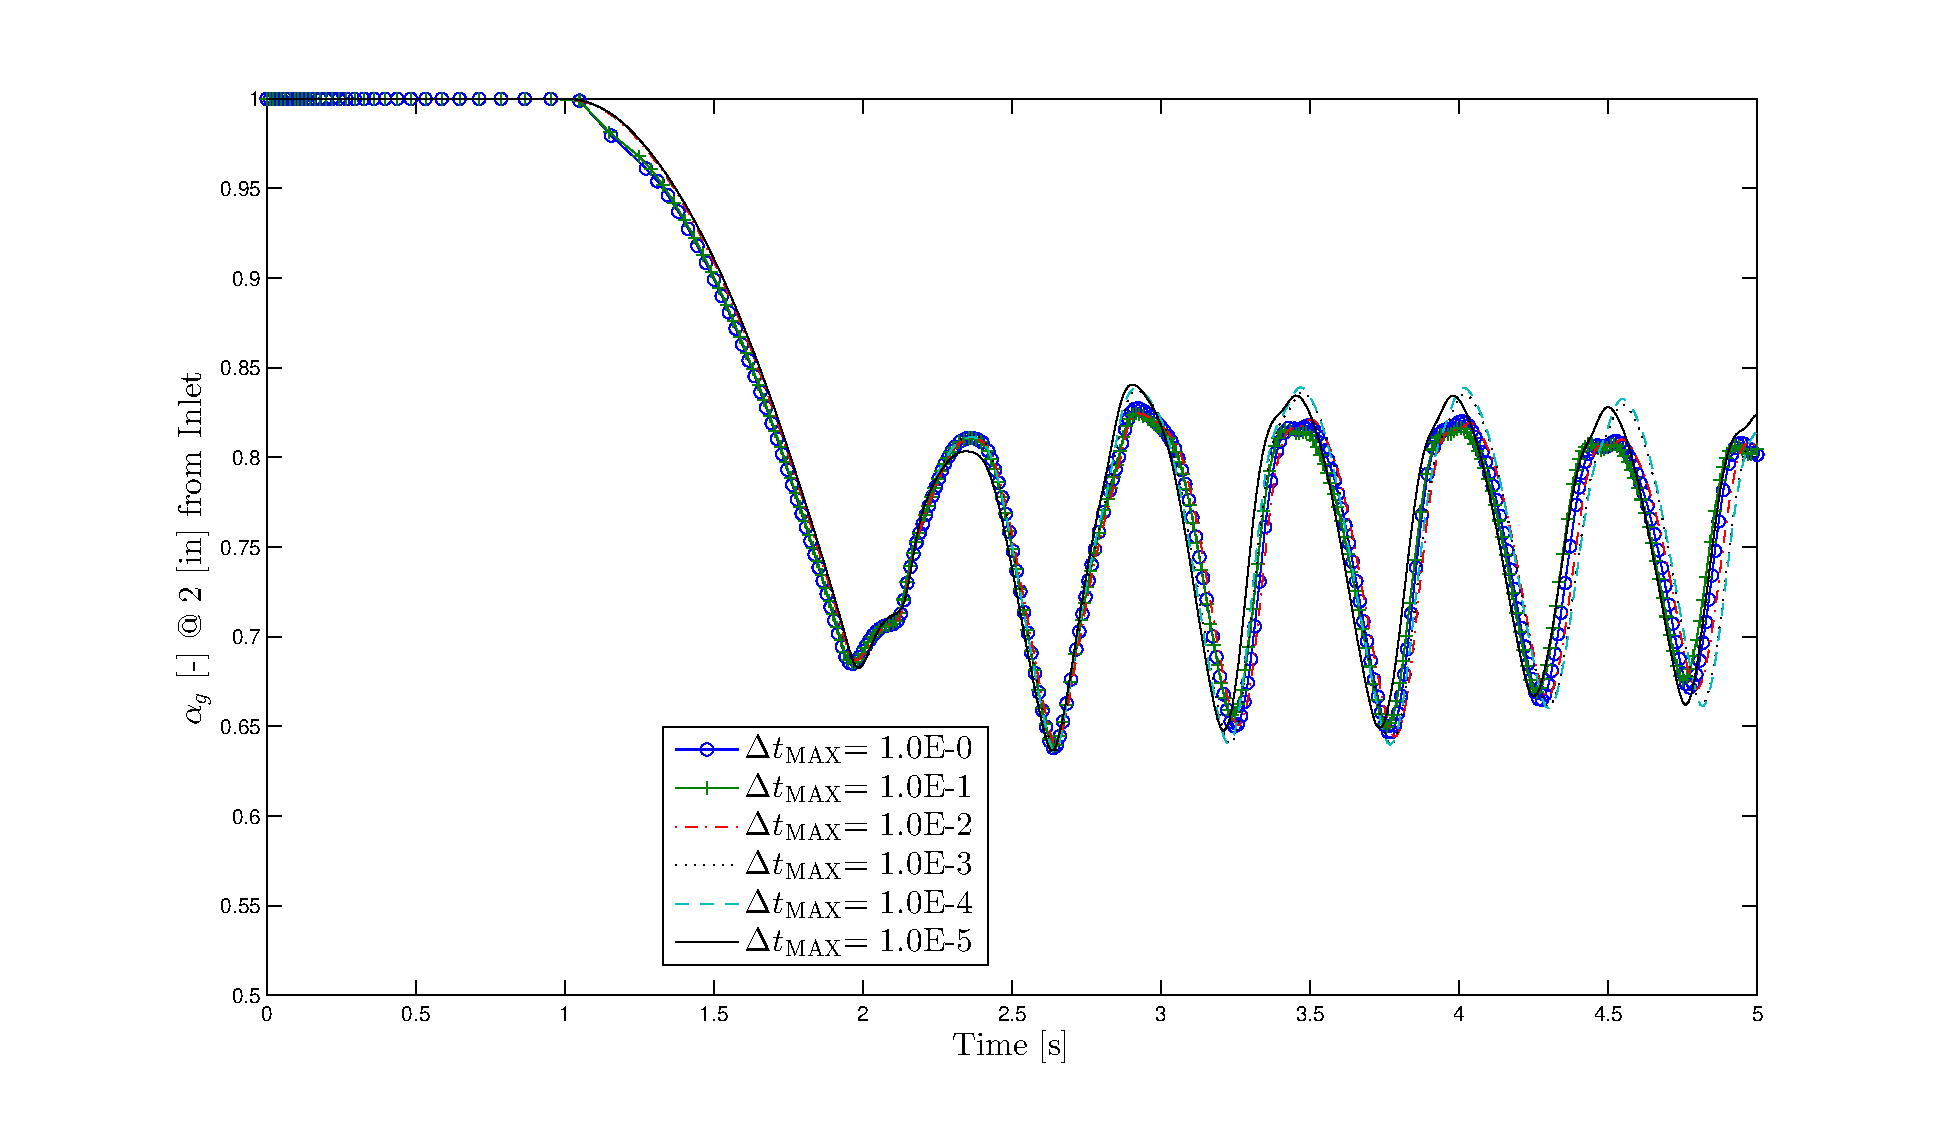
\includegraphics[width=0.49\textwidth]{images/nl_flashing_al_2in.eps}
%\label{fig:nl_mode_flashing}}
%\caption{Flashing simulation.}
%\label{fig:flashing_solutions_1}
%\end{figure}

\begin{figure}[h!t]
\centering
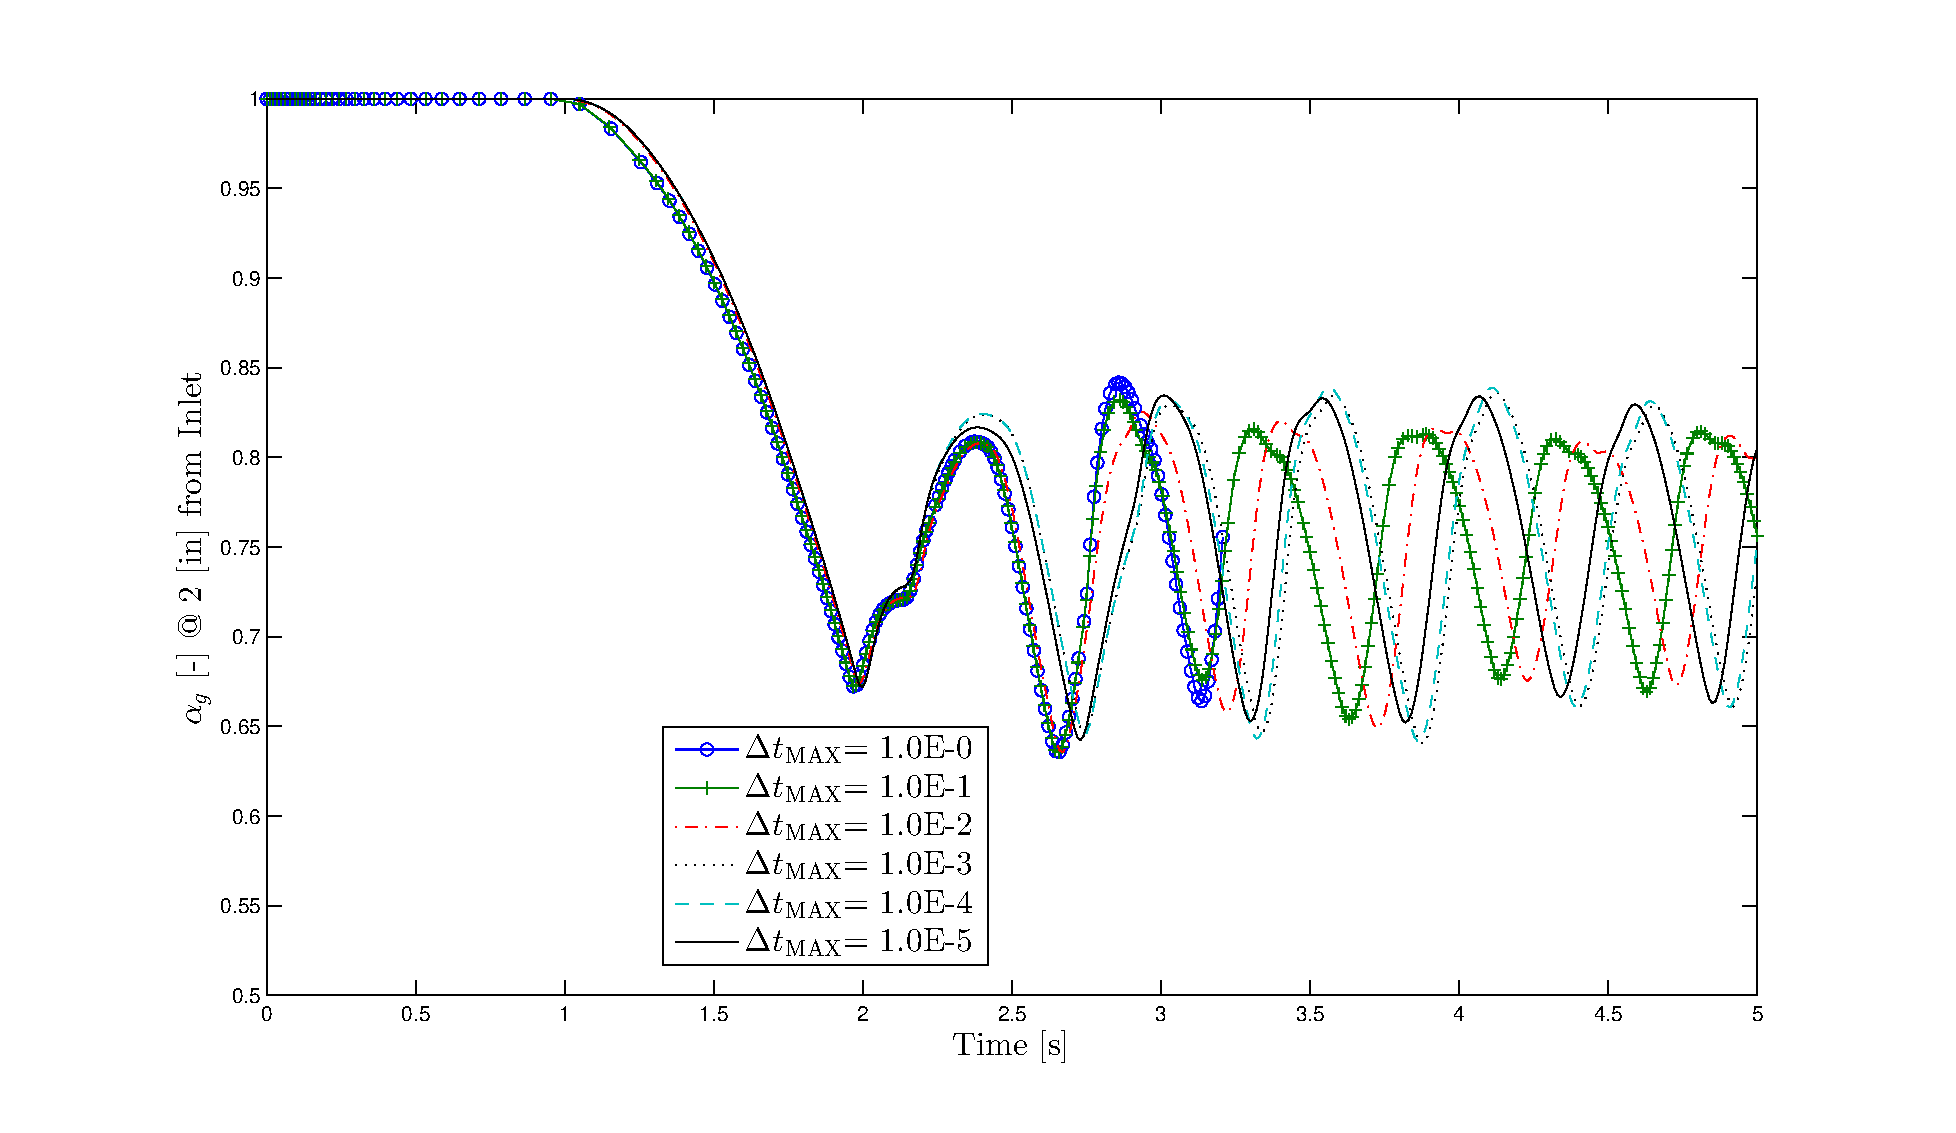
\includegraphics[width=.94\textwidth]{images/cobra_flashing_al_2in.eps}
\caption{Legacy solver flashing solution.}
\label{fig:cobra_mode_flashing}
\end{figure}

\begin{figure}[h!t]
\centering
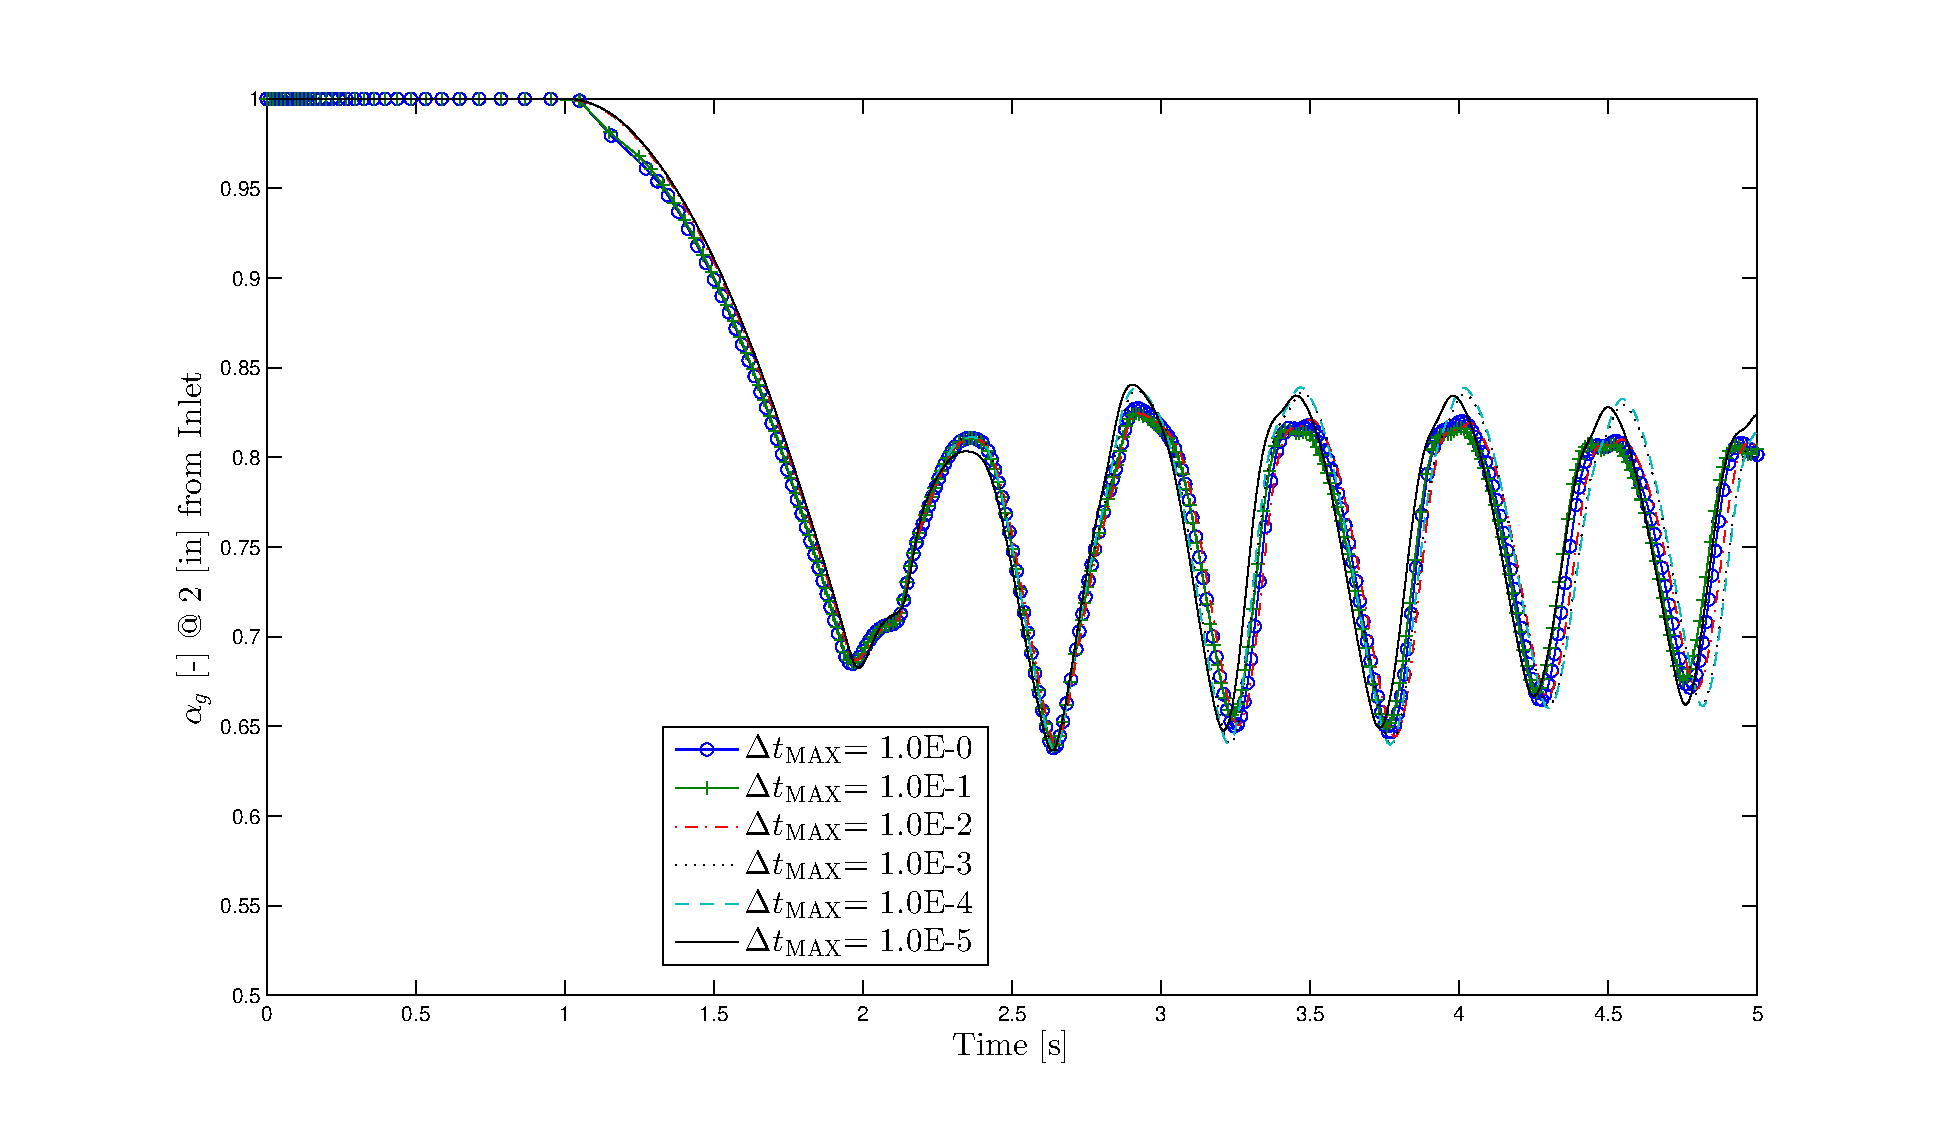
\includegraphics[width=.94\textwidth]{images/nl_flashing_al_2in.eps}
\caption{Nonlinear solver flashing solution.}
\label{fig:nl_mode_flashing}
\end{figure}

The two solvers, when applied to the same problem that contains highly nonlinear physics, produce two different timestep size invariant solutions.
These two solutions achieve qualitative timestep size invariance at different timestep sizes.
The parameter of interest in the solution produced by the nonlinear solver with a 1 [s] $\Delta t_{\text{MAX}}$ is qualitatively close to that produced with a 0.1 [s] $\Delta t_{\text{MAX}}$, \fig{fig:nl_flashing_compare}.
The same level of qualitative timestep size invariance is achieved in the legacy solver solutions between a \dtmax{} of 1.0E-3 [s] and 1.0E-4 [s], \fig{fig:cobra_flashing_compare}.

%\begin{figure}[h!t]
%\centering
%\subfloat[Nonlinear mode solution.]{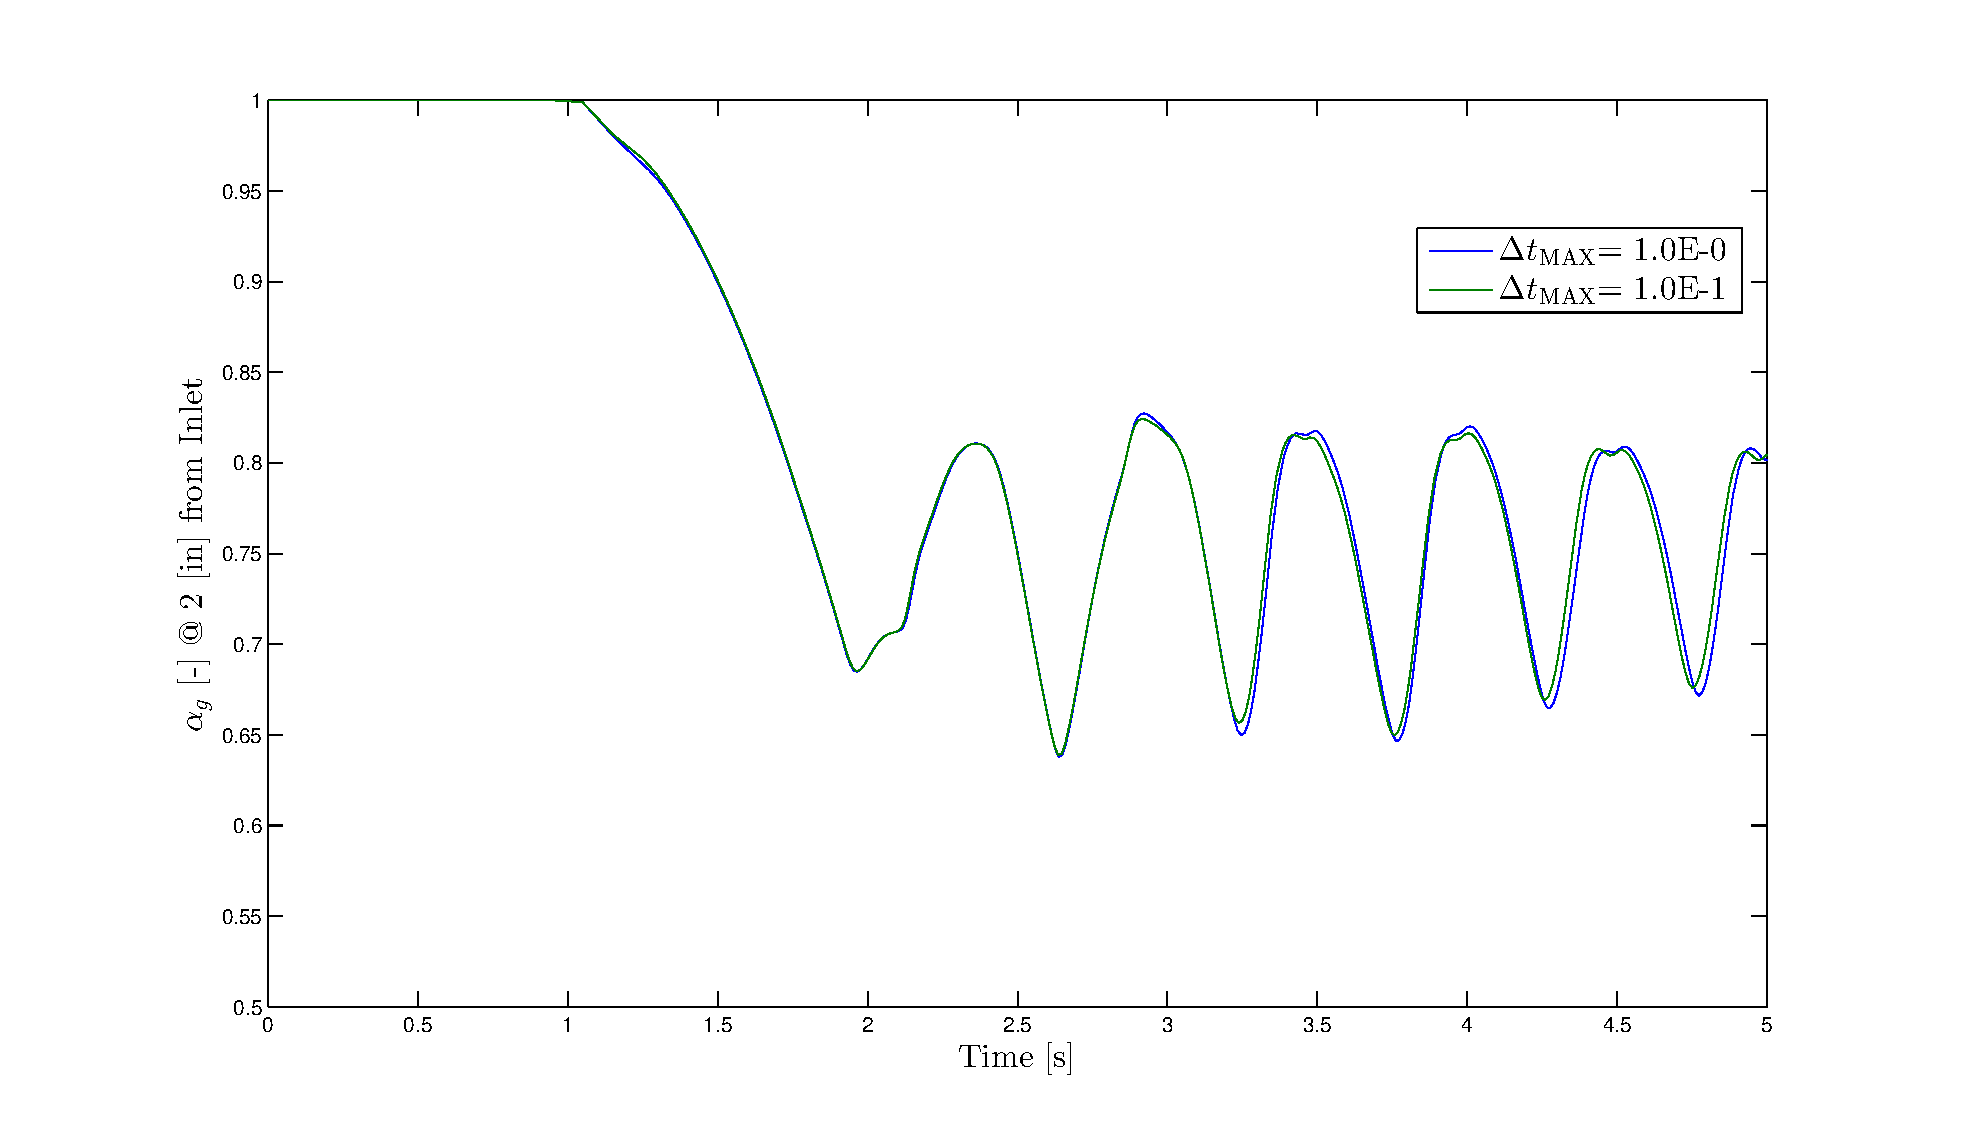
\includegraphics[width=0.49\textwidth]{images/nl_flashing_1em0_1em1.eps}
%\label{fig:nl_flashing_compare}}
%\subfloat[Legacy mode solution.]{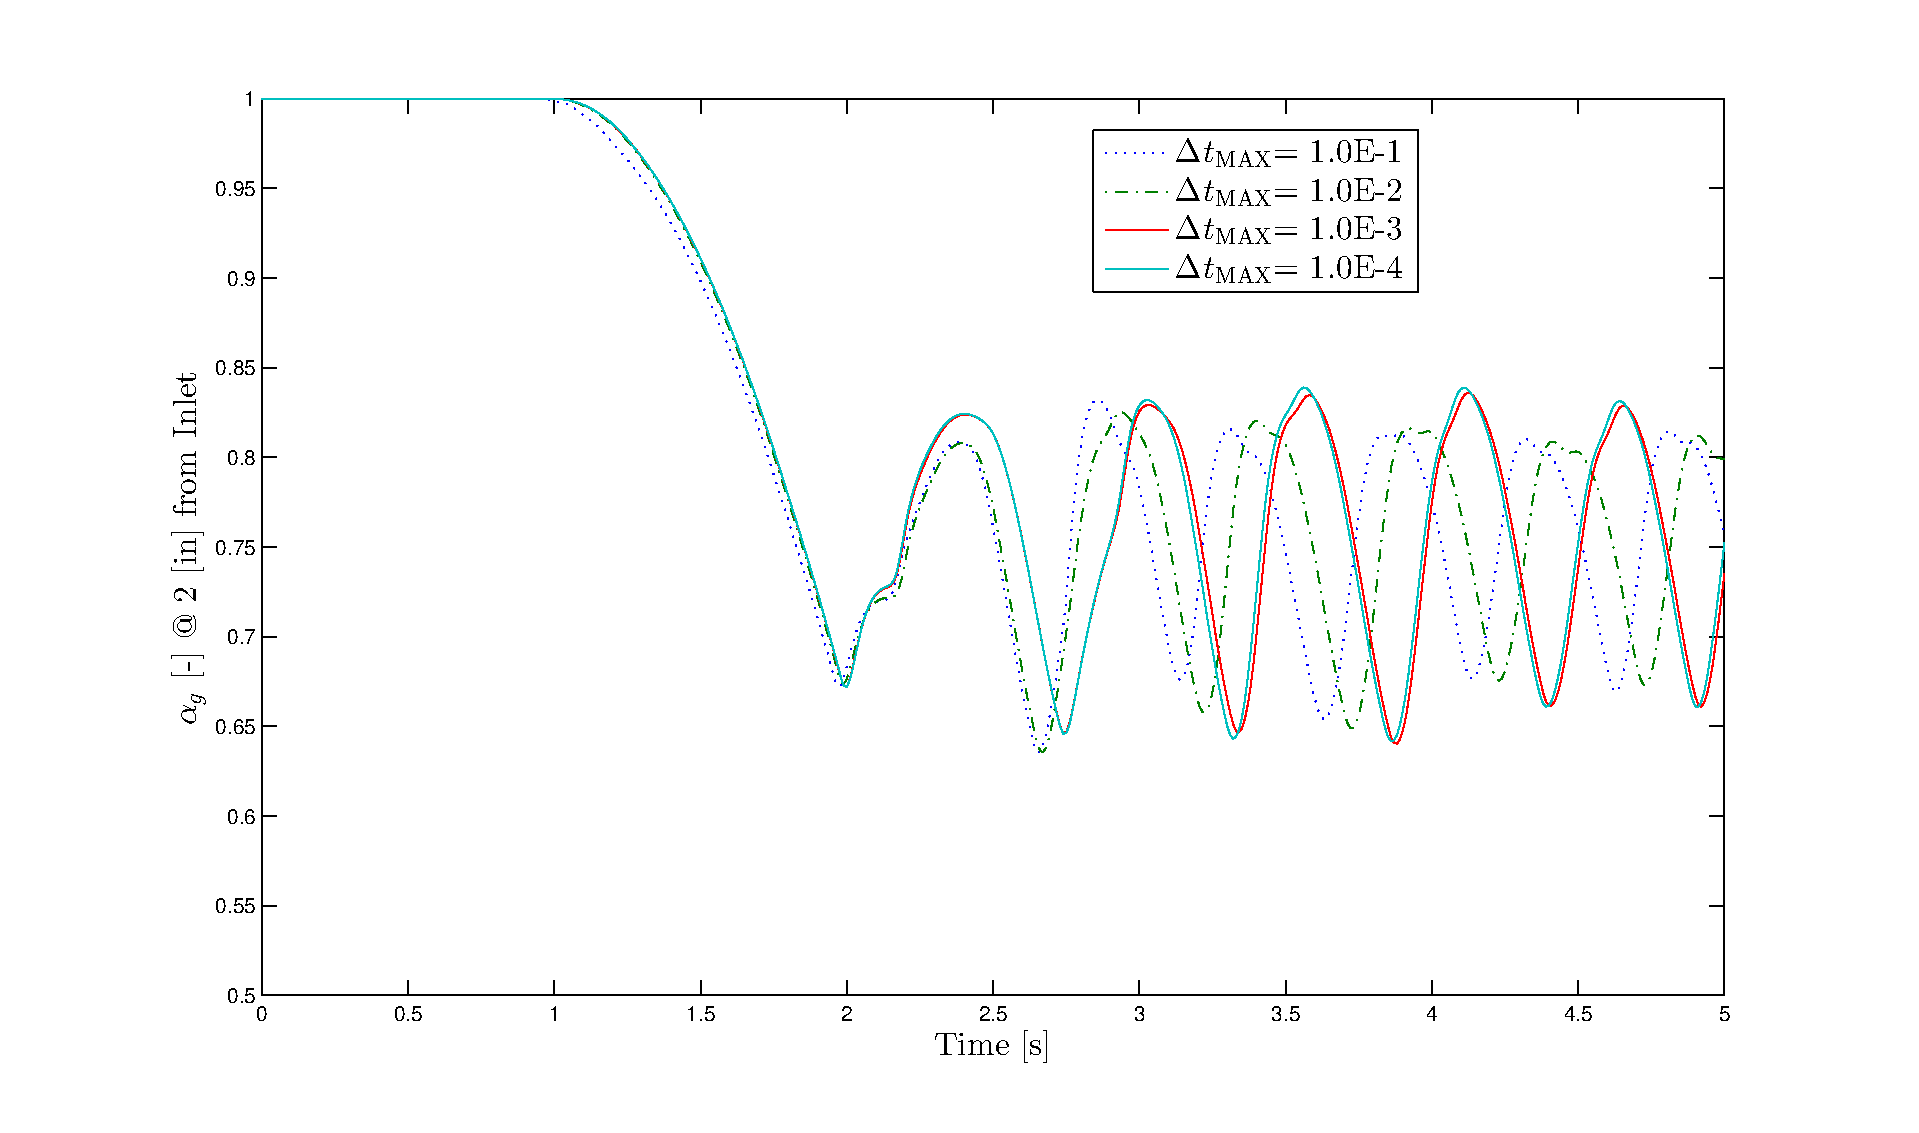
\includegraphics[width=0.49\textwidth]{images/cobra_flashing_1em1_1em4.eps}
%\label{fig:cobra_flashing_compare}}
%\caption{Timestep size insensitive flashing solutions.}
%\label{fig:flashing_res_comp_1}
%\end{figure}

\begin{figure}[h!t]
\centering
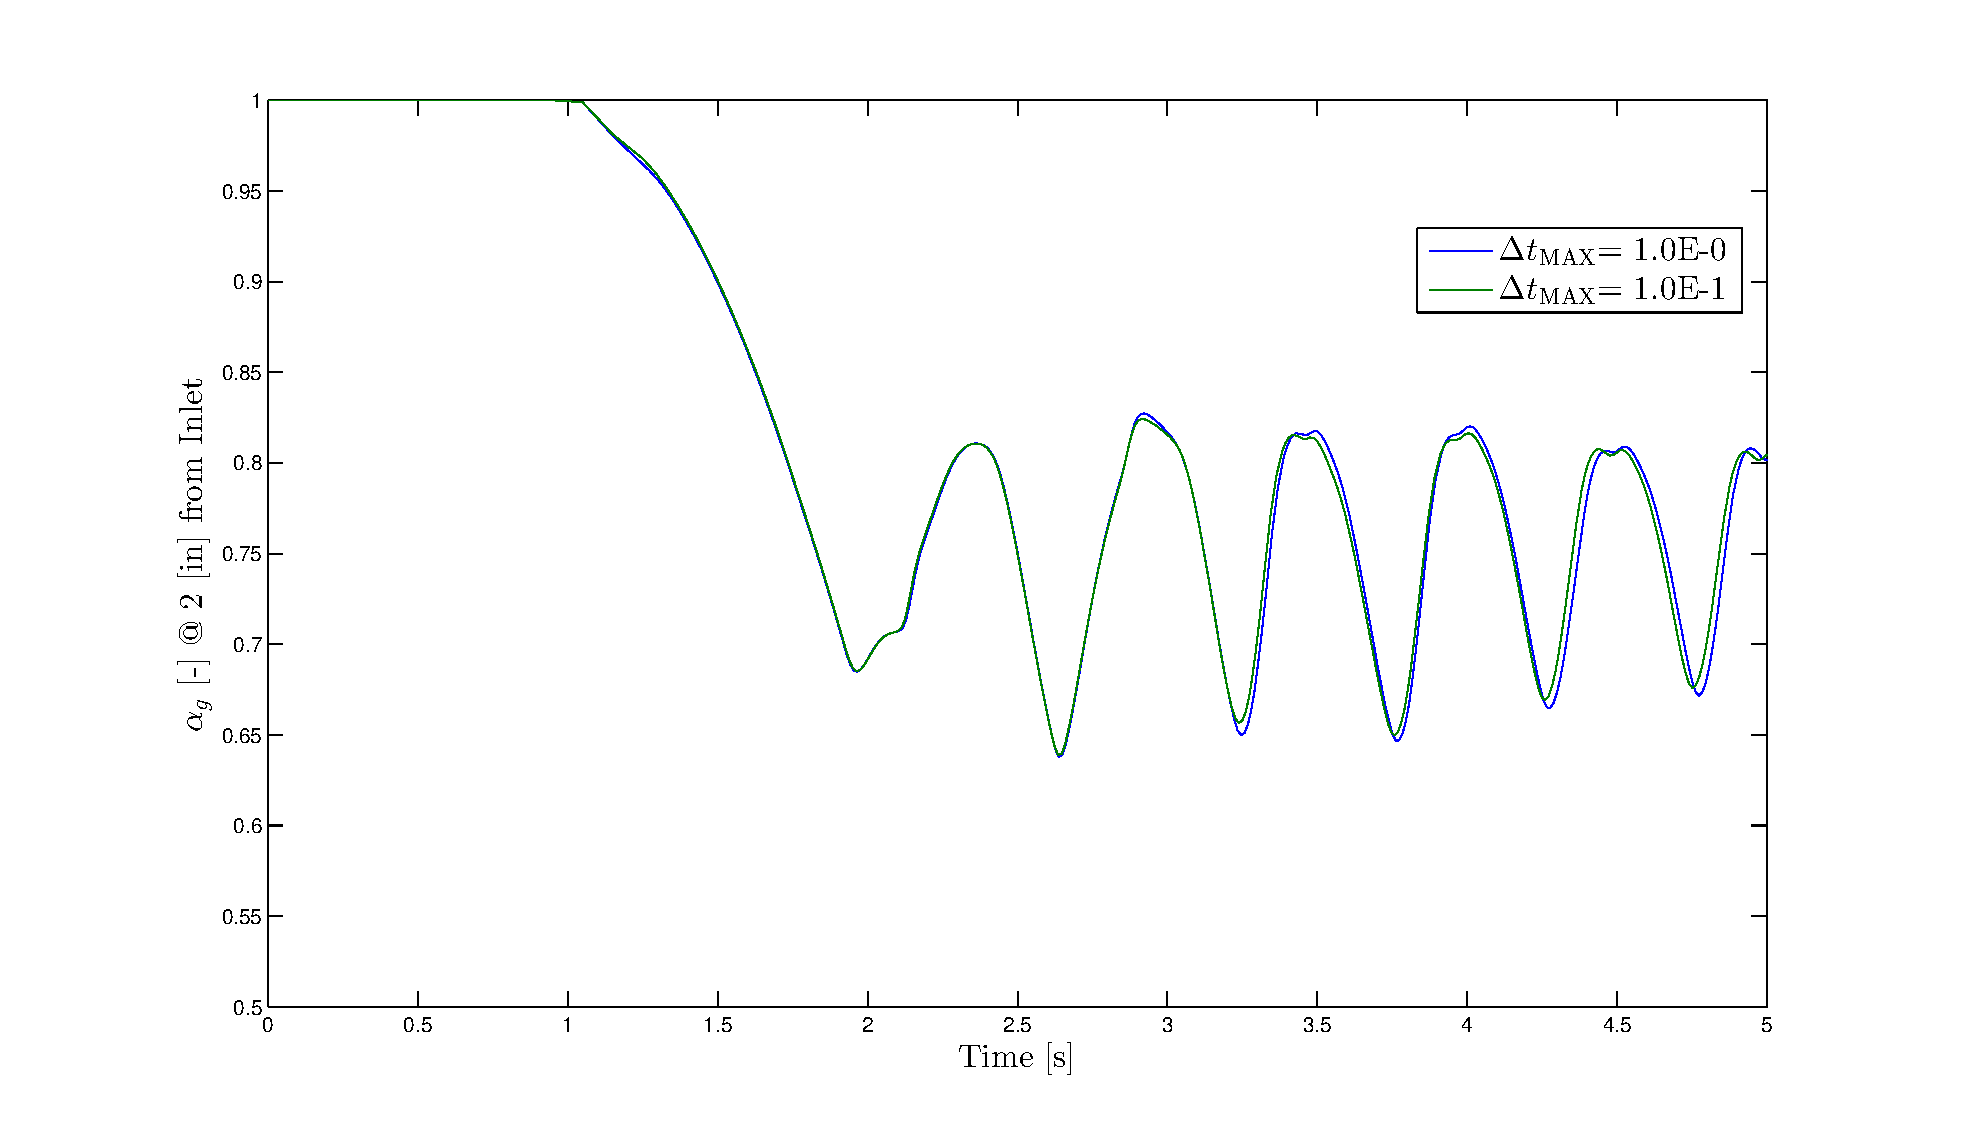
\includegraphics[width=.94\textwidth]{images/nl_flashing_1em0_1em1.eps}
\caption{Nonlinear solver timestep size insensitive flashing solution.}
\label{fig:nl_flashing_compare}
\end{figure}

\begin{figure}[h!t]
\centering
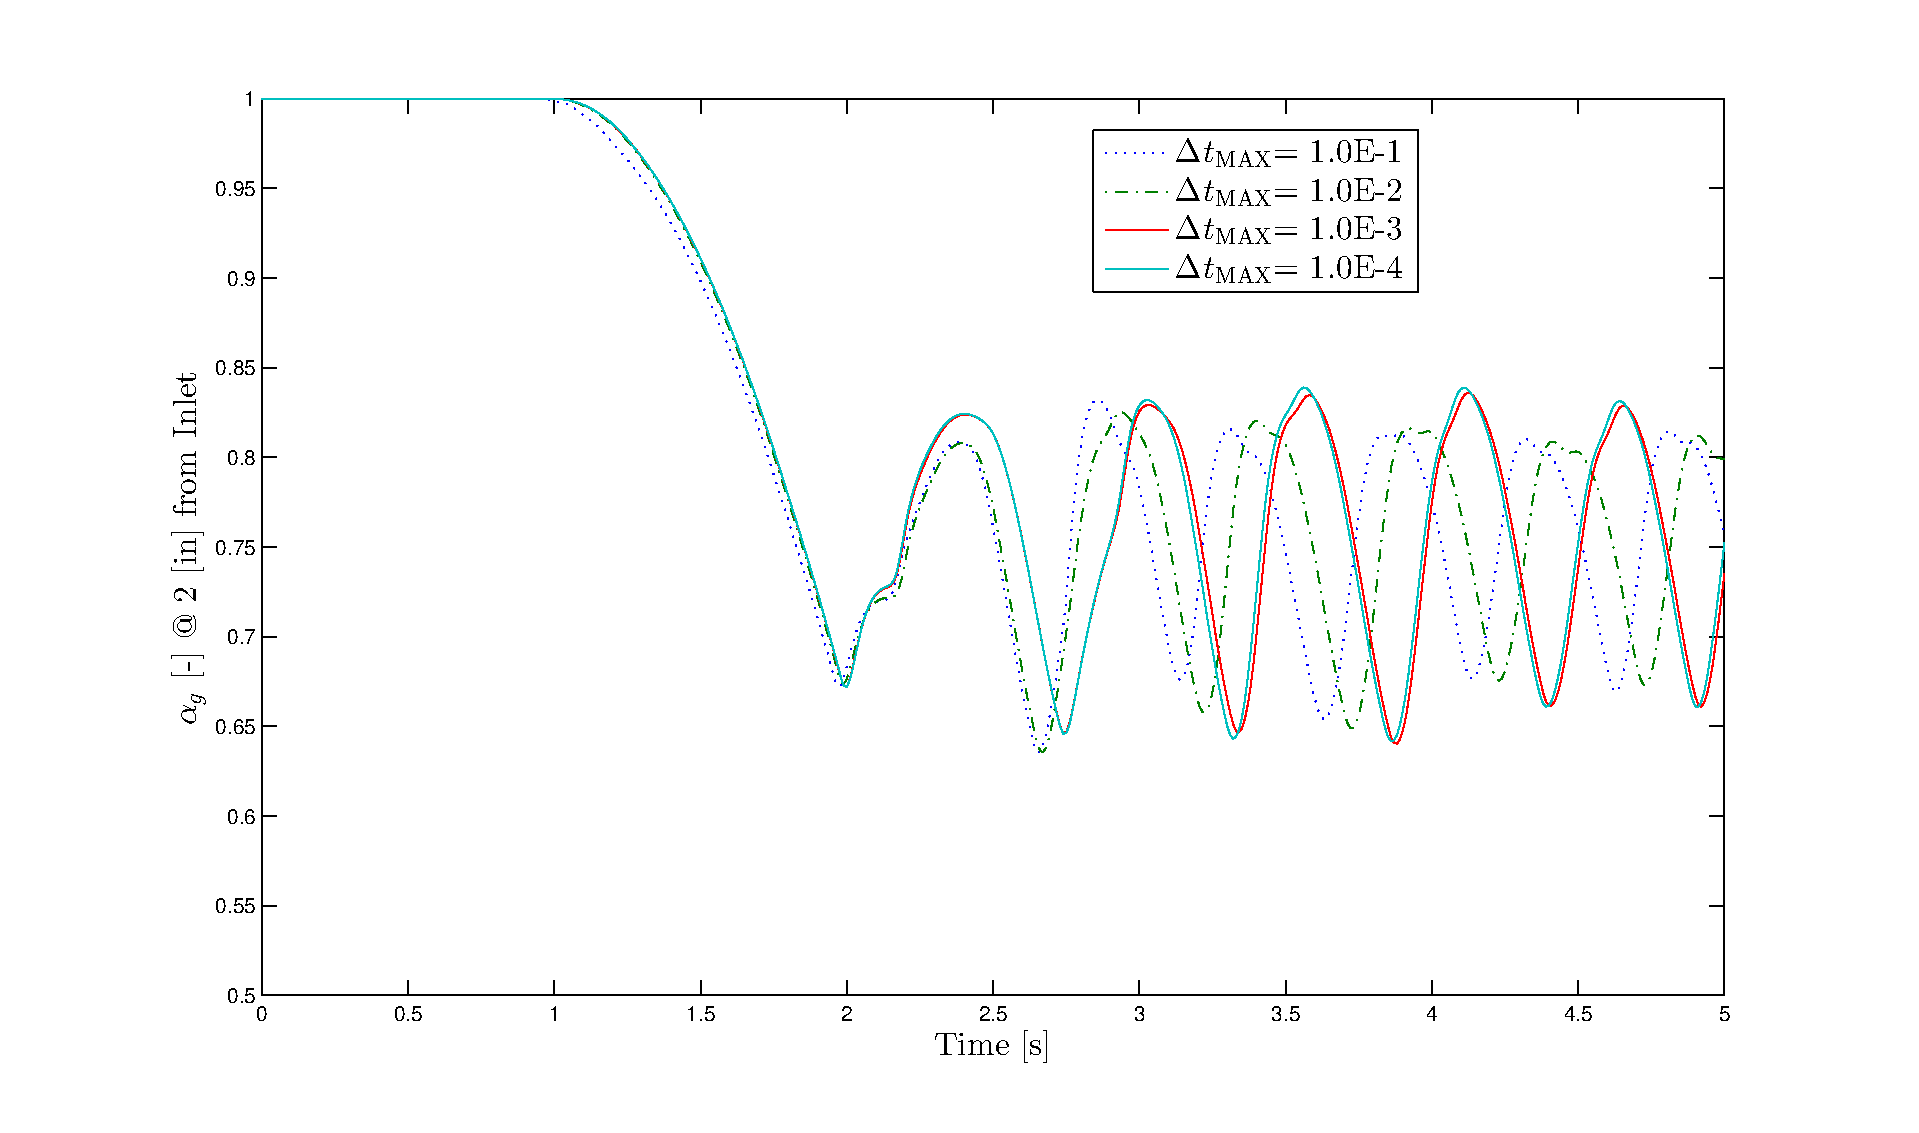
\includegraphics[width=.94\textwidth]{images/cobra_flashing_1em1_1em4.eps}
\caption{Legacy solver timestep size insensitive flashing solution.}
\label{fig:cobra_flashing_compare}
\end{figure}

The timestep size insensitive solution produced by the nonlinear solver occurs at a maximum timestep size three orders of magnitude greater than that achieved by the legacy solver in \cobra{}.
An examination of the nonlinear residual over the course of the transient provides insight into why this behavior is observed.
The scaled residual for the legacy flashing problem indicates that, even for small timestep sizes, the solution obtained still does not satisfy the discrete nonlinear equations, \fig{fig:legacy_flashing_residual}.
This is in contrast to the nonlinear flashing problem, which shows a lower residual over the course of the simulation, \fig{fig:nonlinear_flashing_residual}.

%\begin{figure}[h!t]
%\centering
%\subfloat[Legacy solver residuals.]{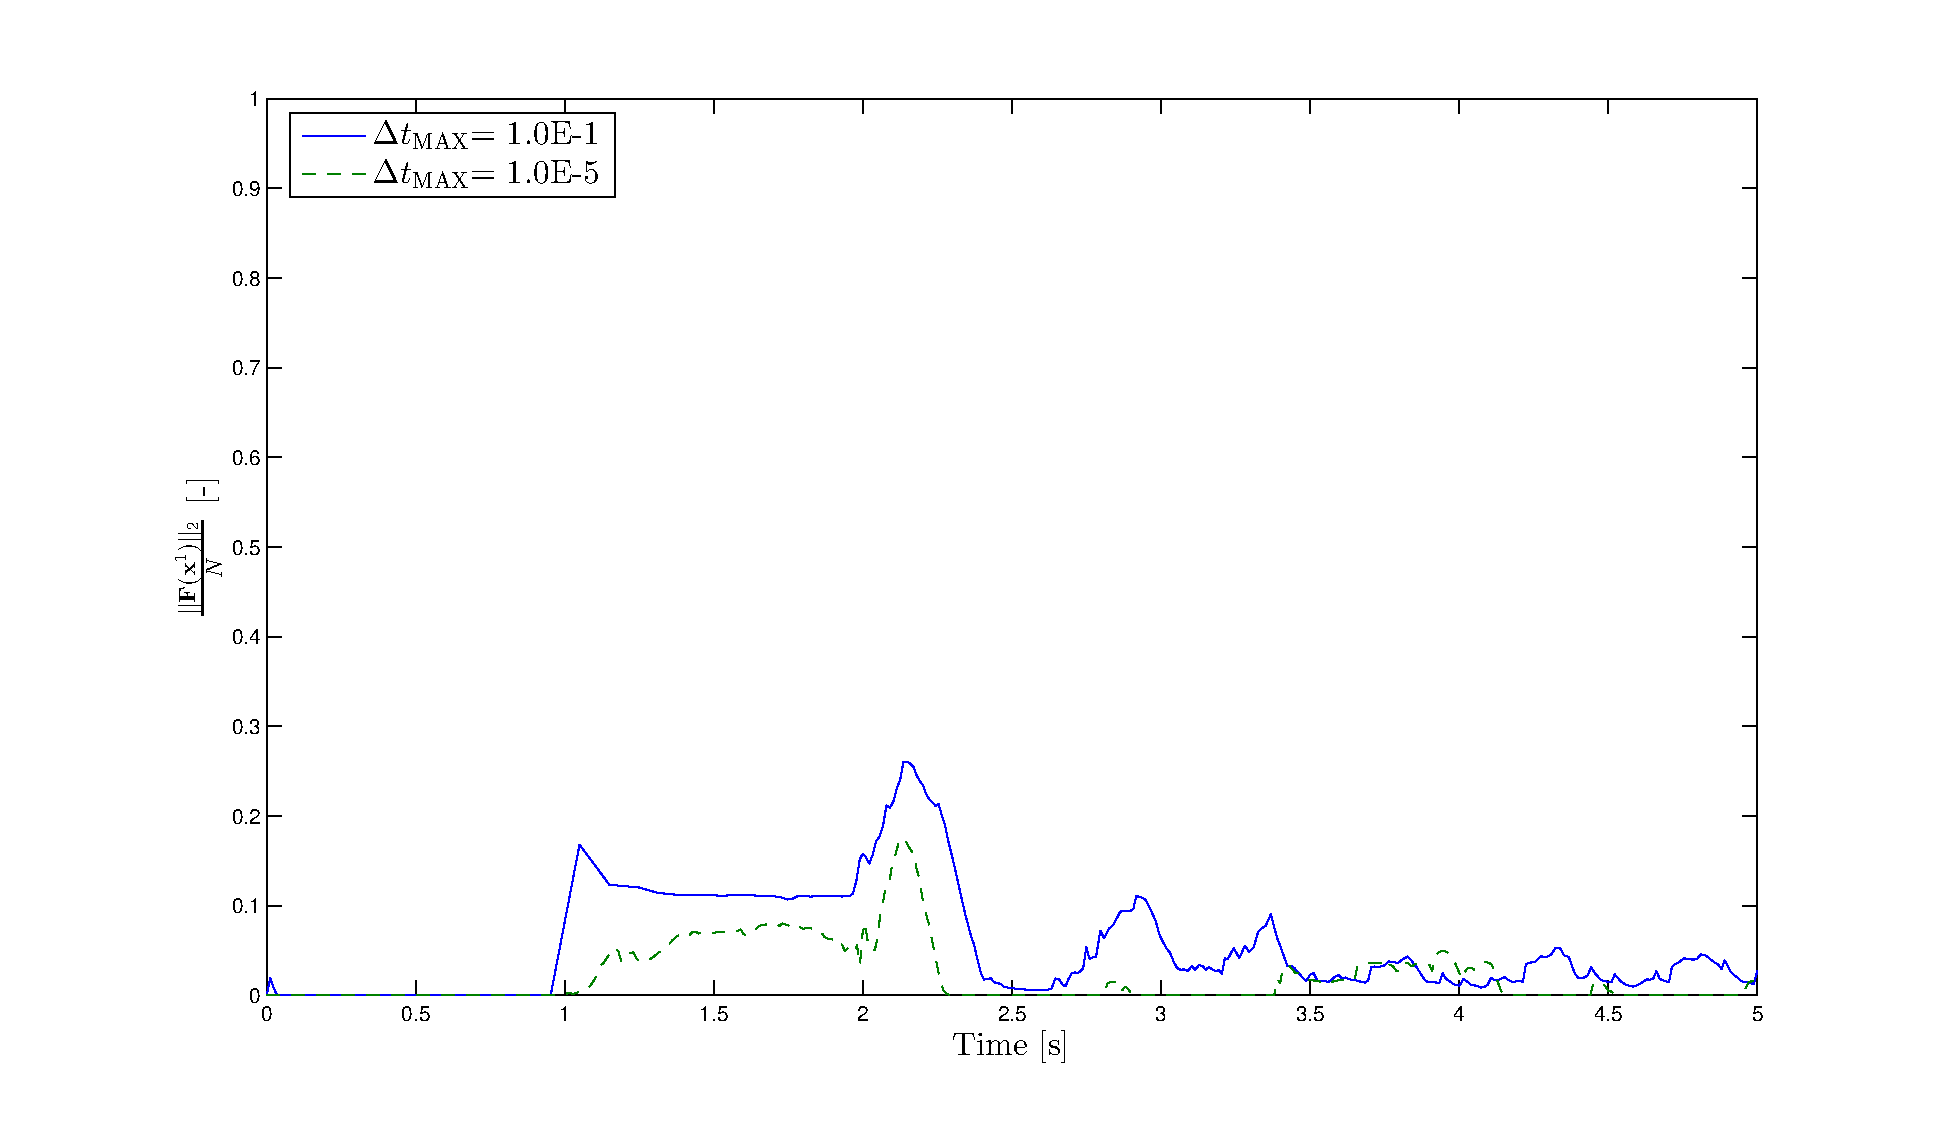
\includegraphics[width=0.49\textwidth]{images/cobra_flashing_res_compare.eps}
%\label{fig:legacy_flashing_residual}}
%\subfloat[Nonlinear solver residuals.]{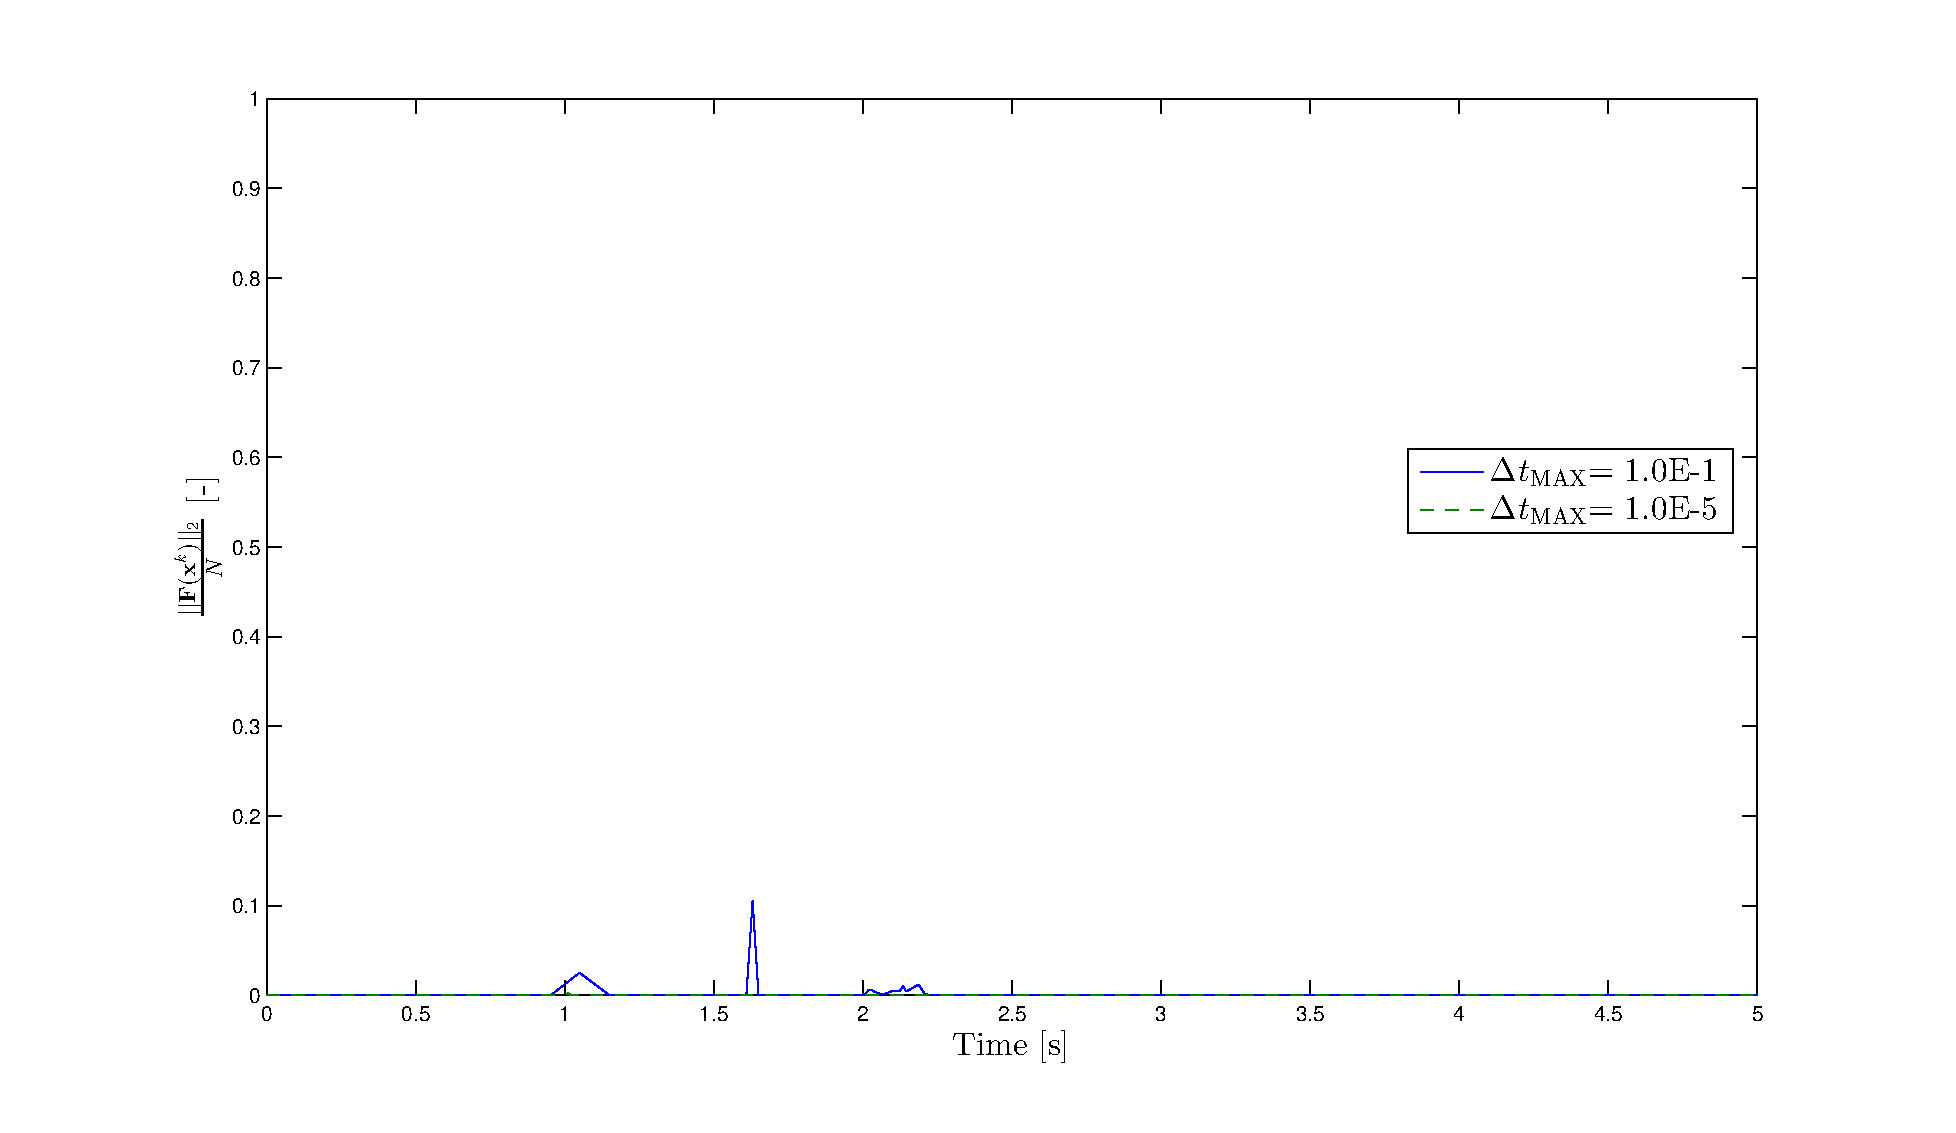
\includegraphics[width=0.49\textwidth]{images/nl_flashing_res_compare.eps}
%\label{fig:nonlinear_flashing_residual}}
%\caption[Flashing residual at $\Delta t_{\text{MAX}}$ = 1.0E-1 {[s]}and 1.0E-5 {[s]}]{Flashing residual at $\Delta t_{\text{MAX}}$ = 1.0E-1 {[s]} and 1.0E-5 {[s]}.}
%\label{fig:flashing_compare_2}
%\end{figure}

\begin{figure}[h!t]
\centering
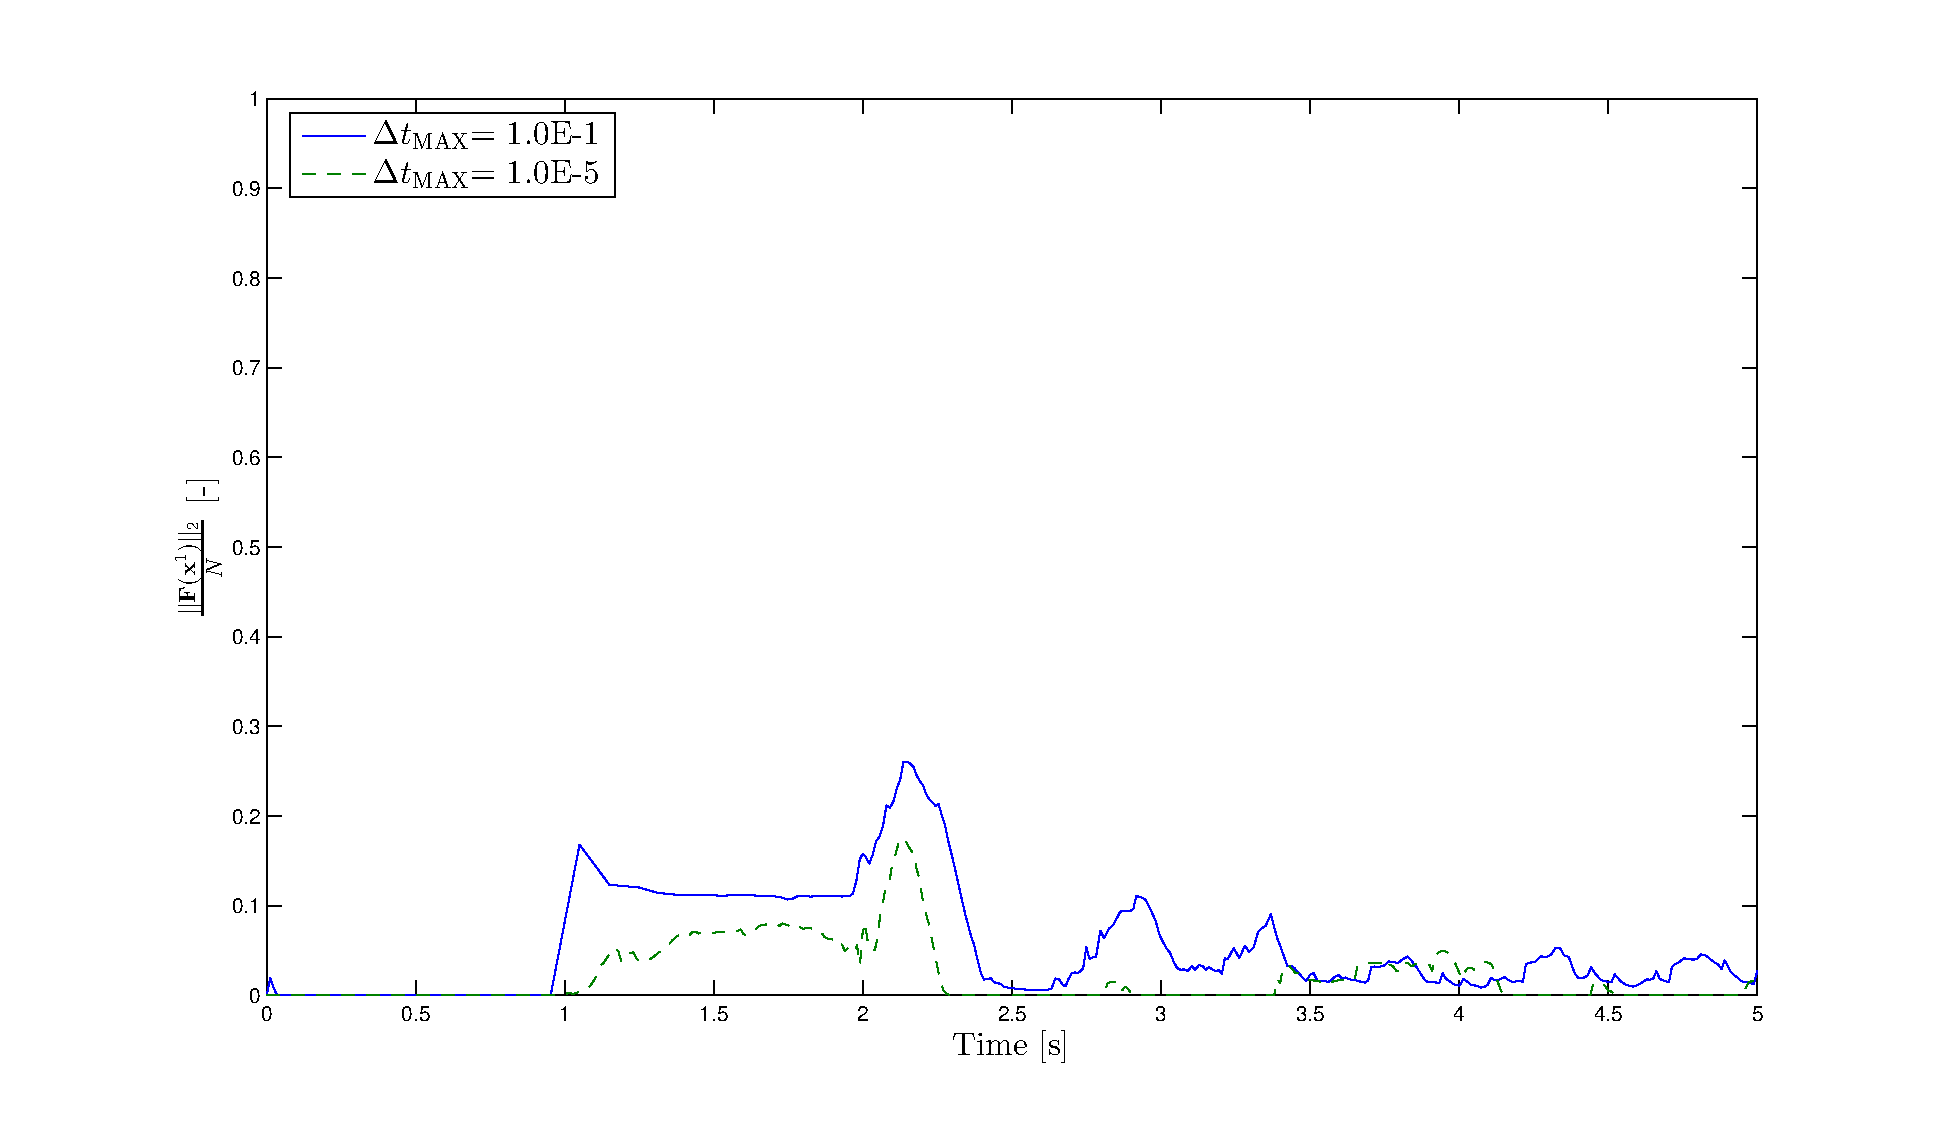
\includegraphics[width=0.94\textwidth]{images/cobra_flashing_res_compare.eps}
\caption{Residual of the flashing solution for the legacy solver.}
\label{fig:legacy_flashing_residual}
\end{figure}

\begin{figure}[h!t]
\centering
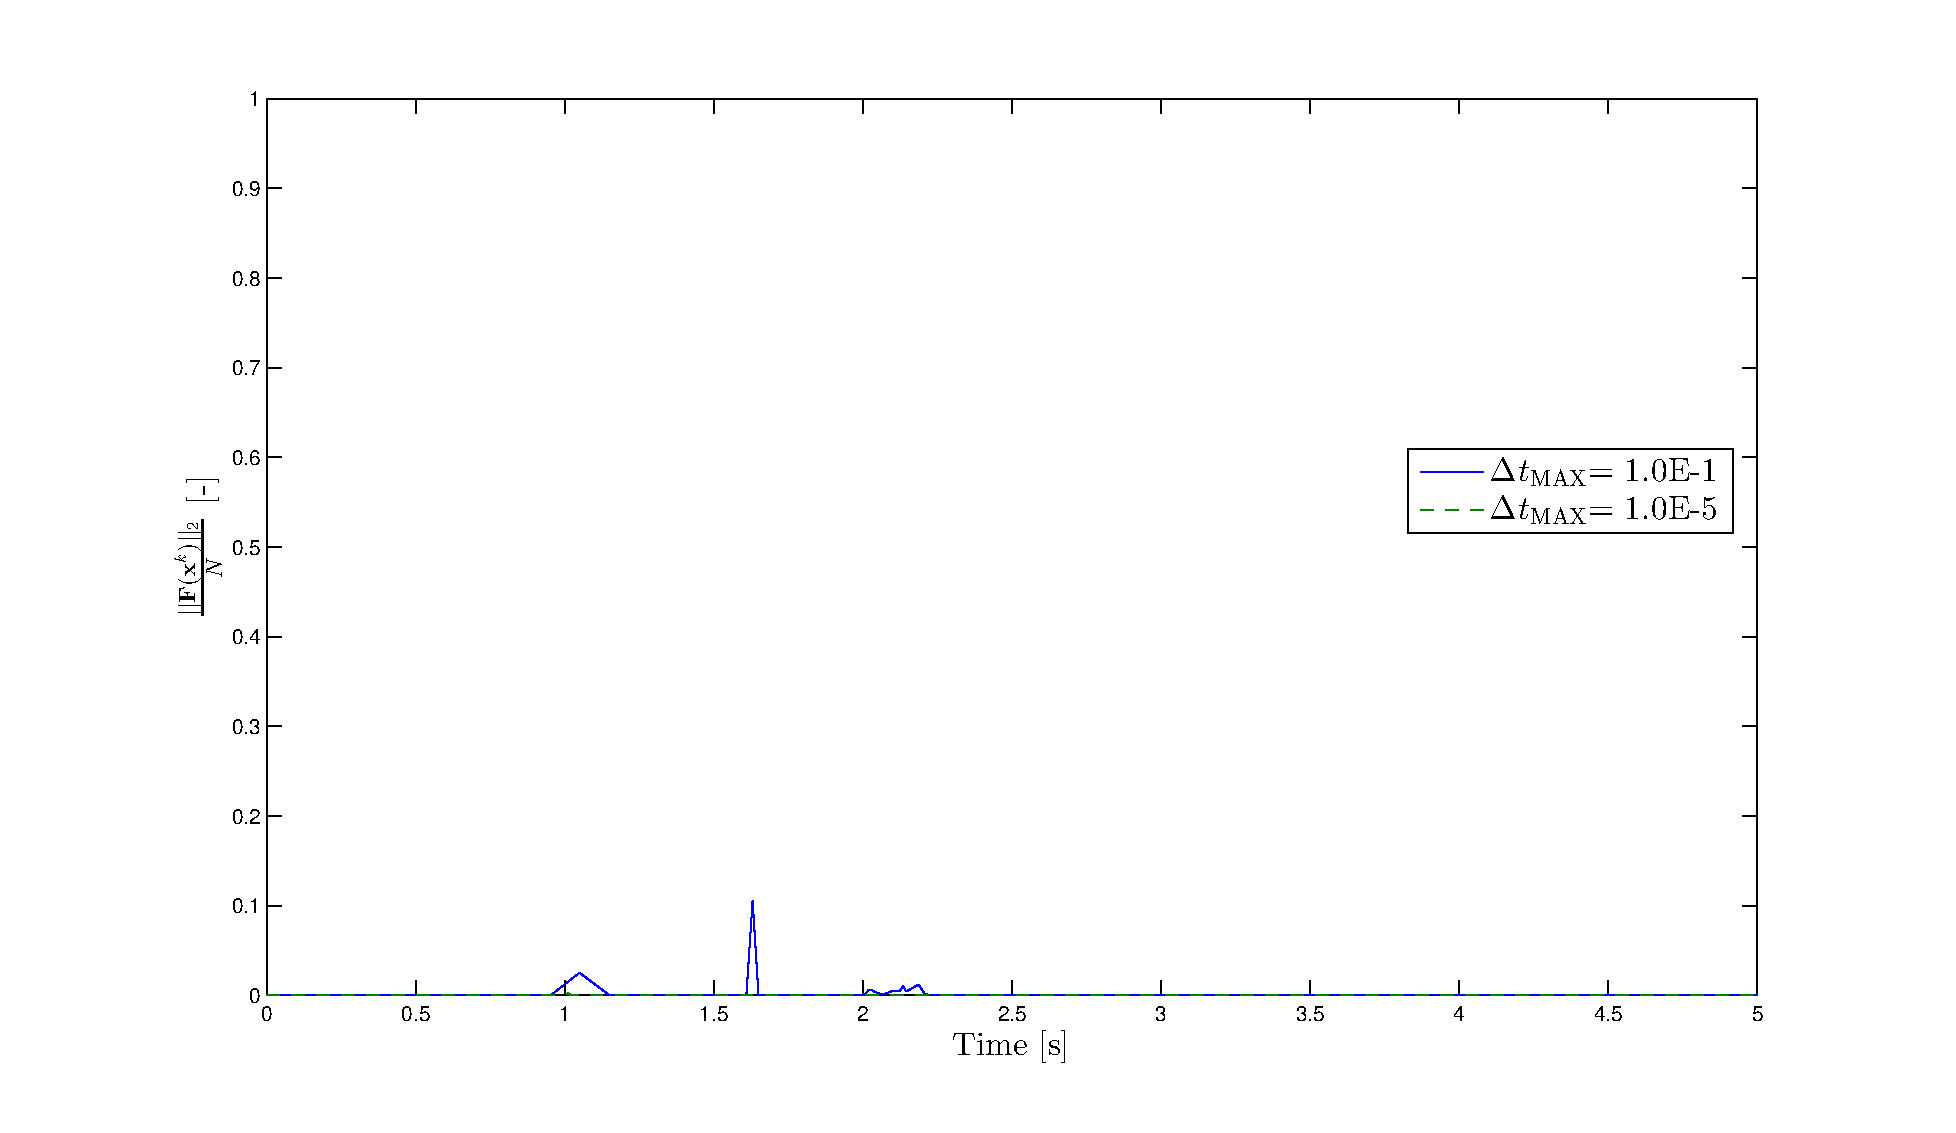
\includegraphics[width=0.94\textwidth]{images/nl_flashing_res_compare.eps}
\caption{Residual of the flashing solution for the nonlinear solver.}
\label{fig:nonlinear_flashing_residual}
\end{figure}

The reduction in the residual exhibited by the solution produced by the legacy solver, \fig{fig:legacy_flashing_residual}, shows that the reduction of the maximum allowable timestep size now serves two purposes.
The first is that as \dtmax{} is reduced the nonlinear physics are being better resolved; however, even for small maximum allowable timestep sizes, the residuals are still large compared to those of the nonlinear solution, \fig{fig:nonlinear_flashing_residual}.
The second purpose in reducing \dtmax{} is to decrease the error due to the discrete approximation of the temporal integral of the governing equations.
While the reduction of the maximum timestep size in the legacy solver serves the purpose of reducing the residual, the nonlinear solver performs this task naturally.
Therefore, in the nonlinear solver the reduction of the maximum timestep size primarily serves to reduce the error from the approximate discrete temporal integral.

During simulations with large \dtmax{} there are three time periods of the transient where the residuals from the nonlinear solver are nontrivial.
These are at the initiation of the inlet flow, during the 1 [s] long ramp to full flow, and after the inlet flow has achieved steady state at 2 [s].
The convergence criteria outlined in \sect{sect:nln_solver:cobra} include two paths through which Newton's method may terminate while having a non-trivial residual.
The first is that the maximum allowable number of Newton iterates, $k_{\text{MAX}}$, may have been exceeded. 
This may indicate that $k_{\text{MAX}}$ may be too small, terminating the iterative process prior to a solution being obtained.
The second is that the norm of the scaled independent parameter update vector may be below its convergence threshold.
A concern is that the update vector produced by the Newton step may be truncated based upon the limiting of the independent parameters at the end of a Newton step.
It may be impossible for the algorithm to reach a nonlinearly converged solution without pushing an independent parameter outside of the acceptable limits imposed by the software.
Since the global minimization problem is not formulated as a constrained minimization problem, there may be inconsistencies in the solution.
This non-convergence of the residual needs additional investigation to determine its cause, its impact upon the algorithmic framework, and its possible remedies.

%\begin{figure}[h!t]
%\centering
%\subfloat[\dtmax{} = 1.0 {[s]}]{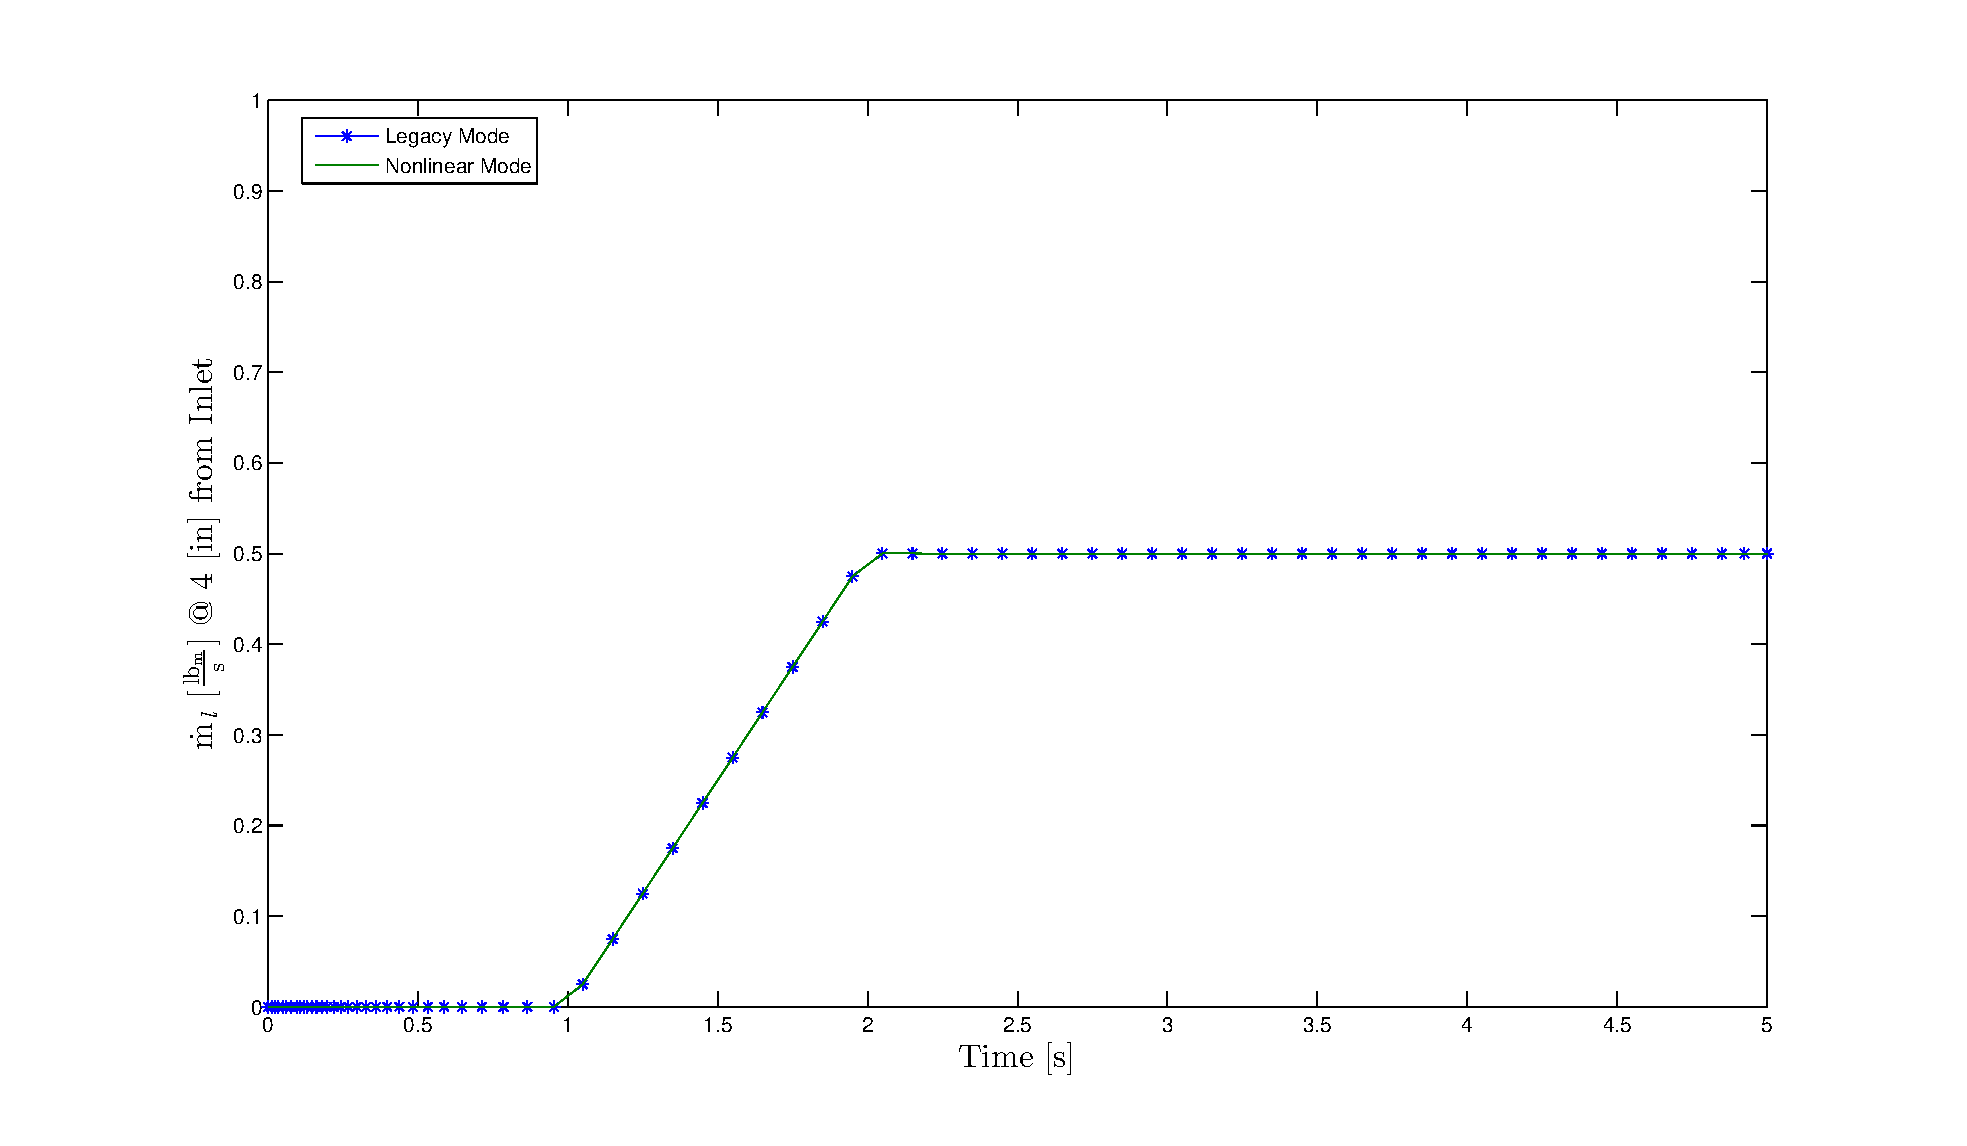
\includegraphics[width=0.49\textwidth]{images/single_1em0.eps}
%\label{fig:single_1em1}}
%\subfloat[\dtmax{} = 1.0E-5 {[s]}]{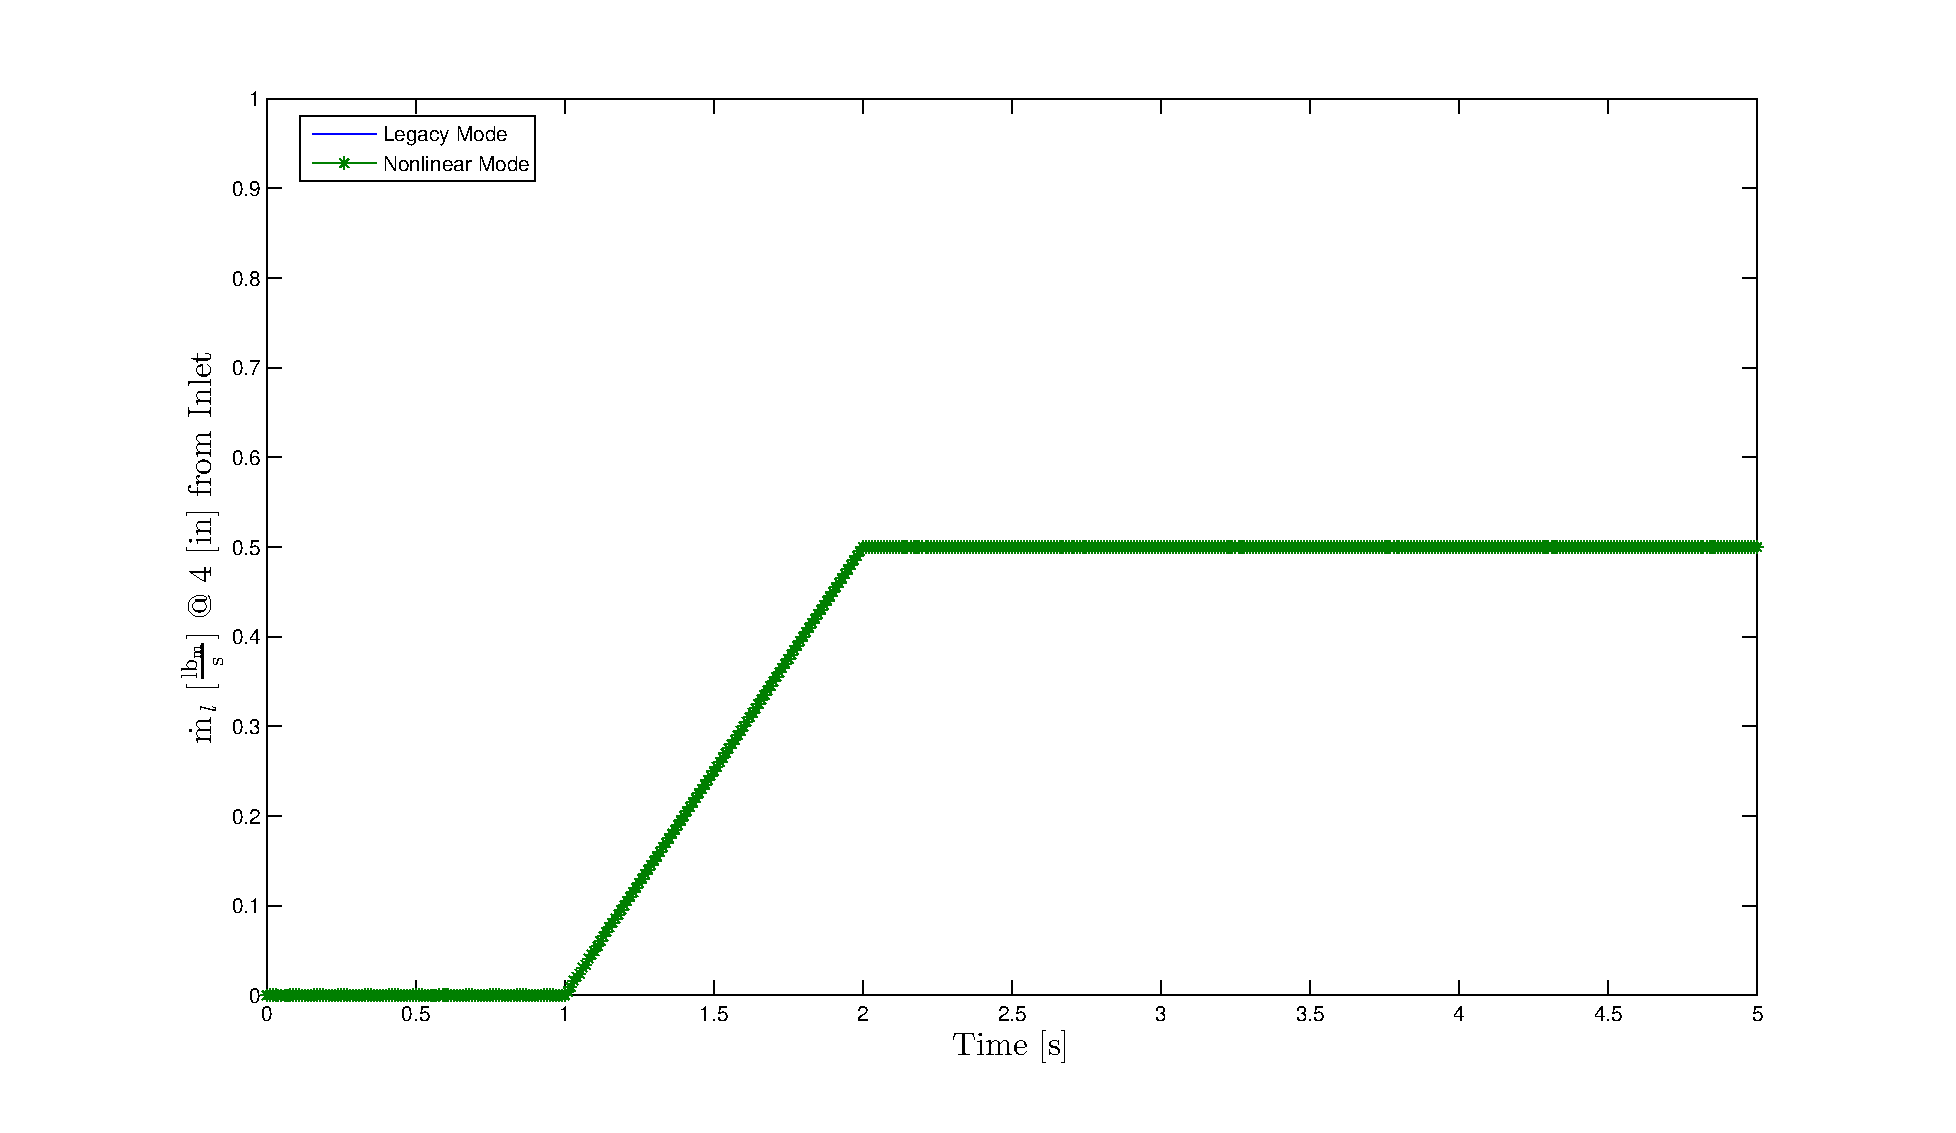
\includegraphics[width=0.49\textwidth]{images/single_1em5.eps}
%\label{fig:single_1em5}}
%\caption[Single-phase solution at \dtmax{} = 1.0 {[s]}and 1.0E-5 {[s]}]{Single-phase solution with \dtmax{} = 1.0 {[s]} and 1.0E-5 {[s]}.}
%\label{fig:single_compare_1}
%\end{figure}

\begin{figure}[h!t]
\centering
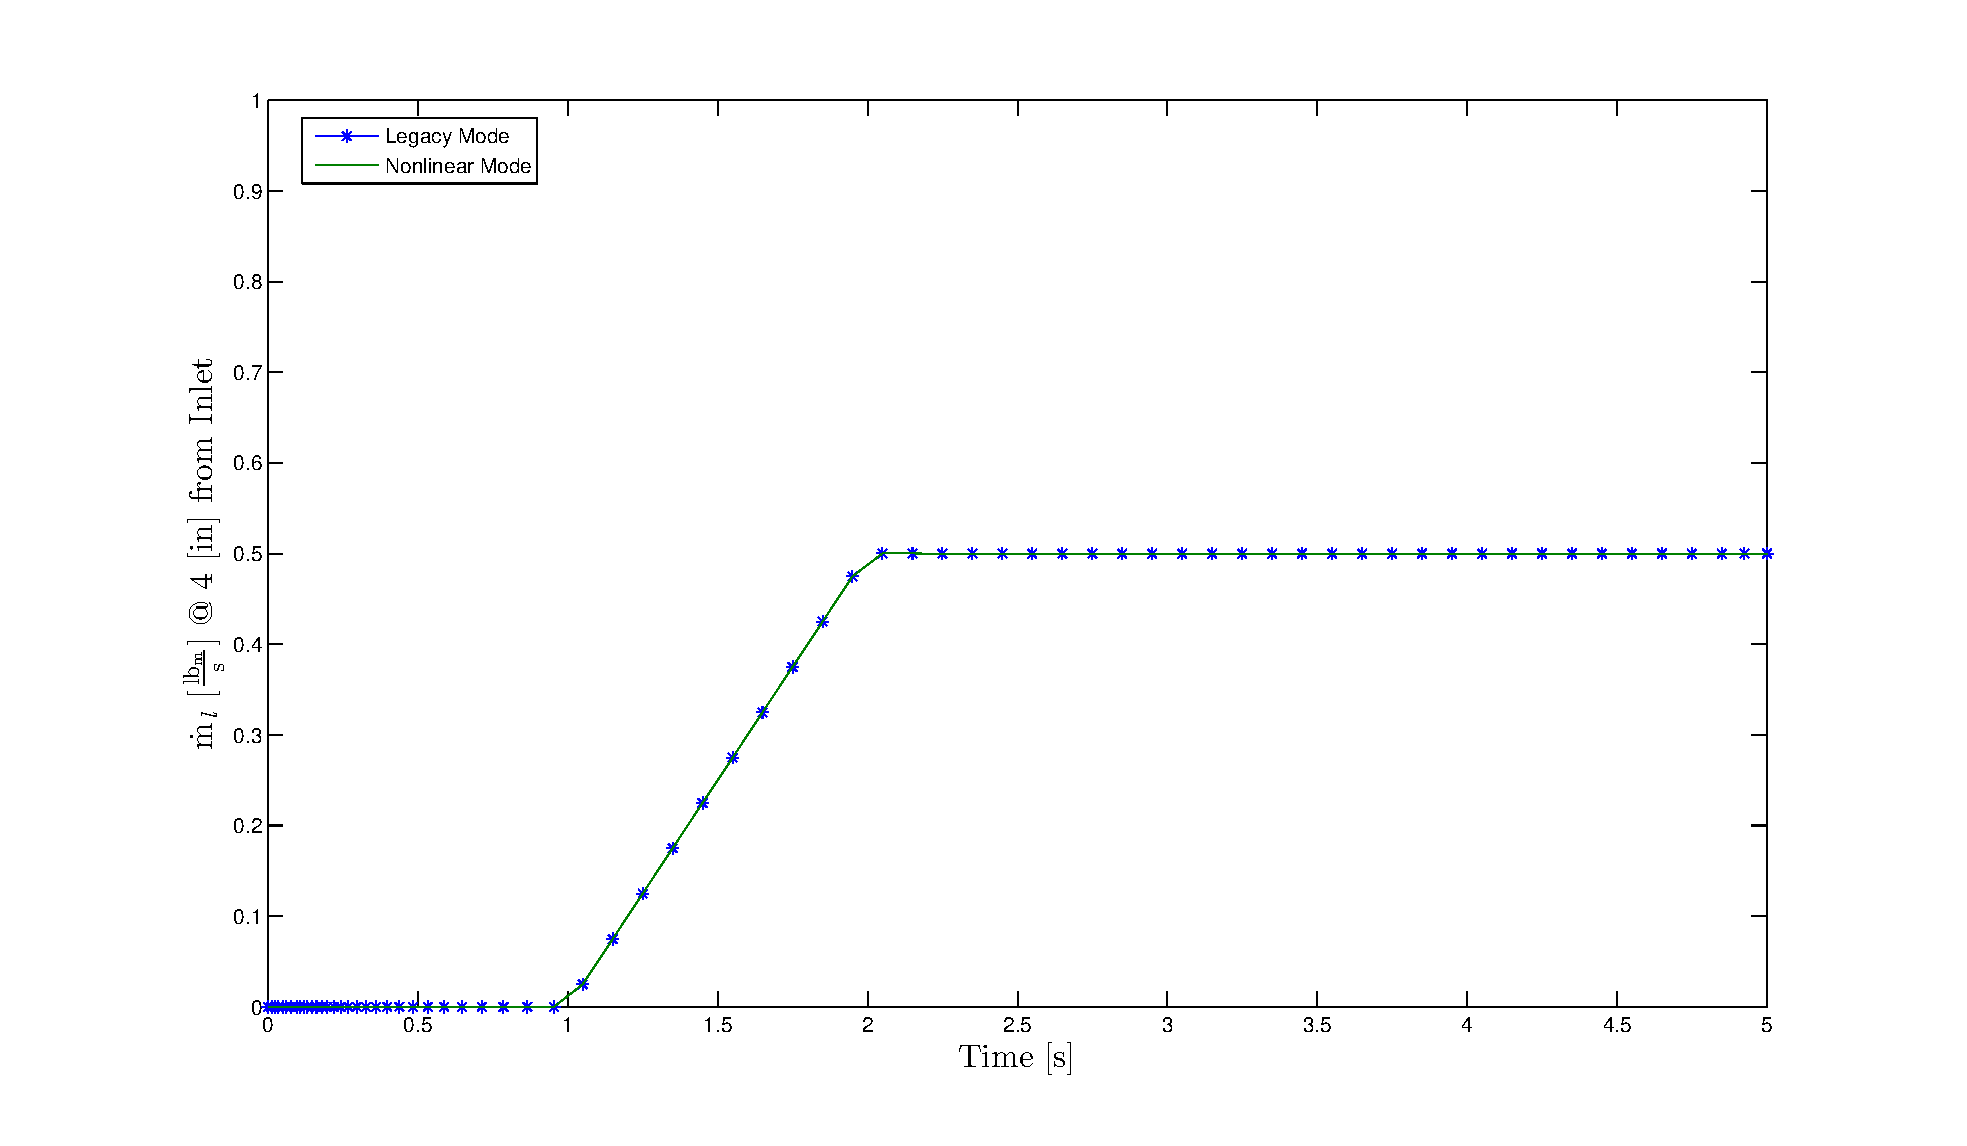
\includegraphics[width=0.94\textwidth]{images/single_1em0.eps}
\caption{Single-phase solution with \dtmax{} = 1.0 {[s]}.}
\label{fig:single_1em1}
\end{figure}

\begin{figure}[h!t]
\centering
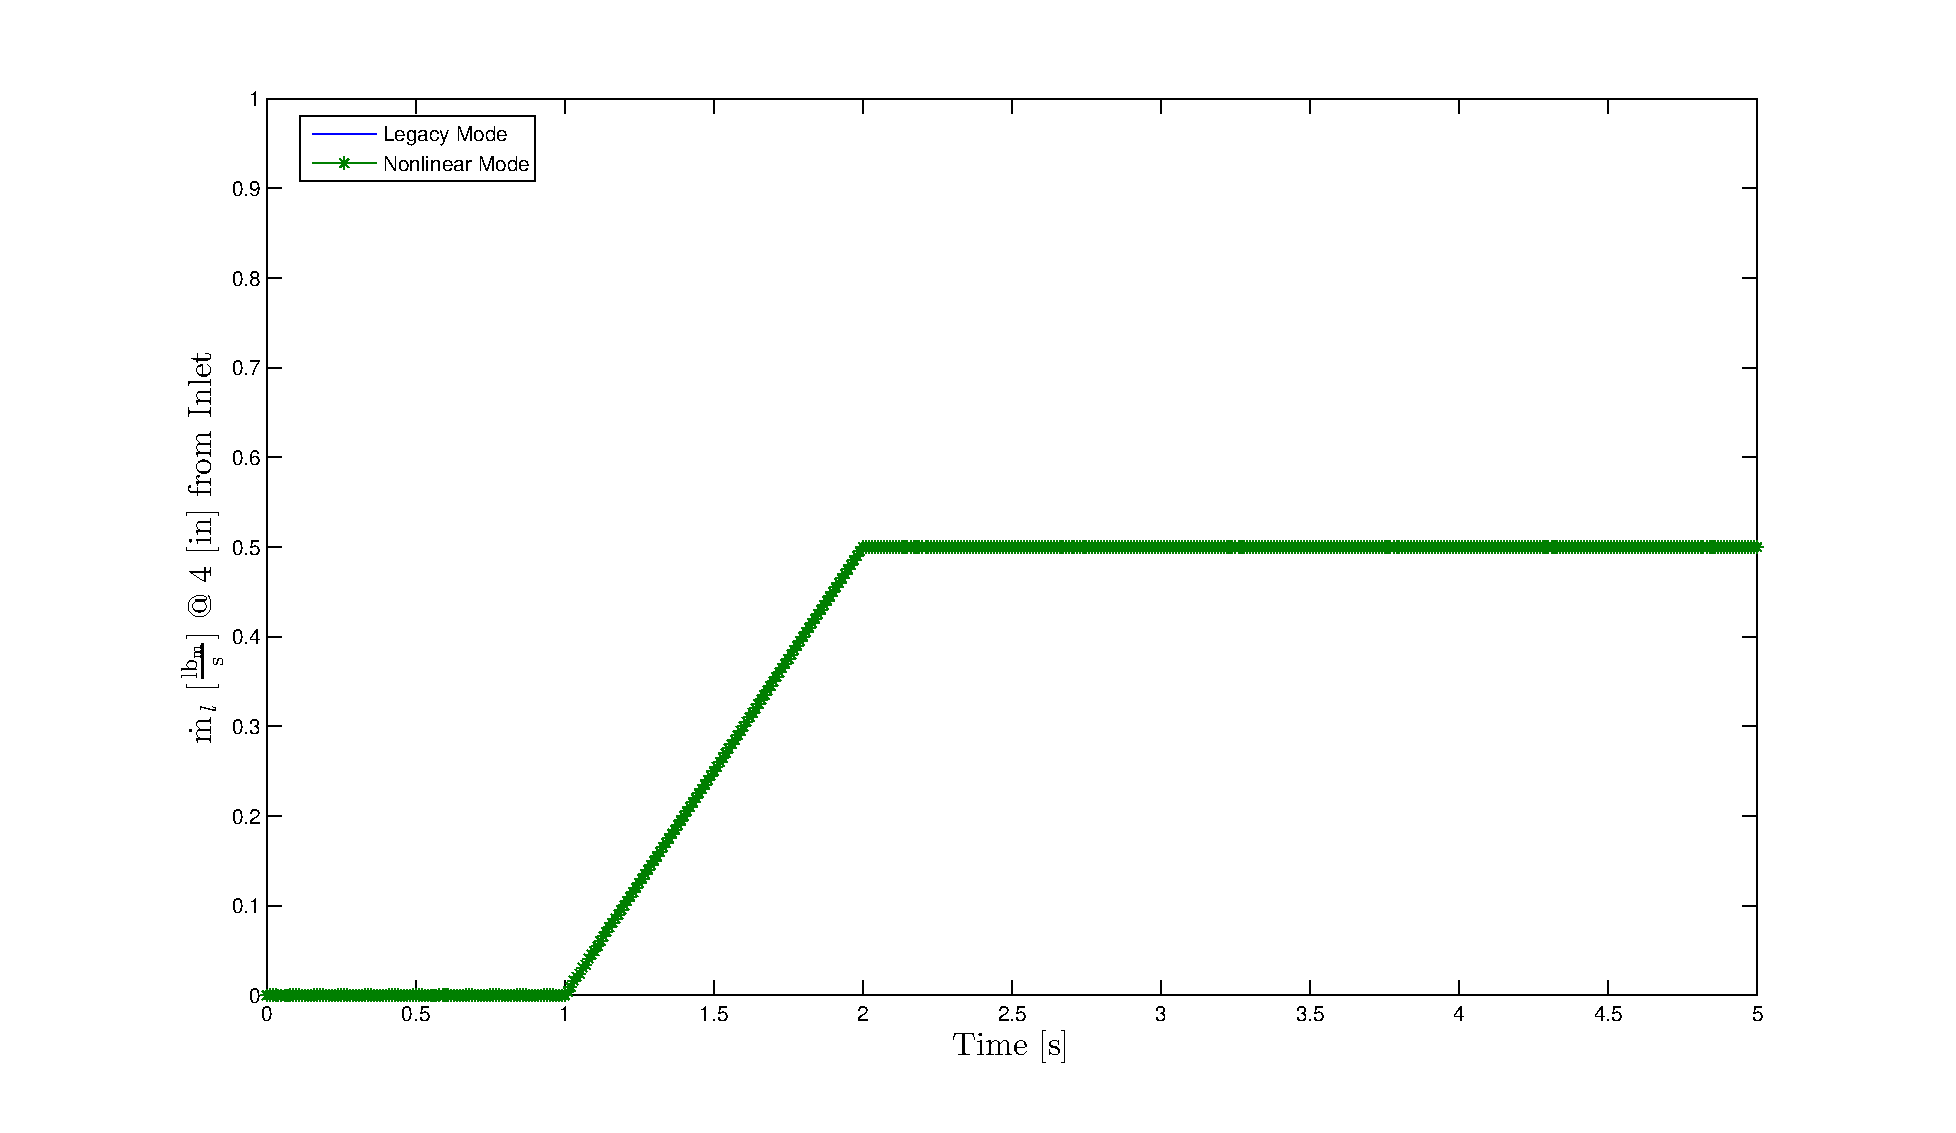
\includegraphics[width=0.94\textwidth]{images/single_1em5.eps}
\caption{Single-phase solution with \dtmax{} = 1.0E-5 {[s]}.}
\label{fig:single_1em5}
\end{figure}

The single-phase case was designed to test if the legacy solver produced a simulation result that was equivalent to that produced by the nonlinear solver.
More specifically, it was designed to show that for problems where the physics of interest have relatively low nonlinearities, the legacy solver provides as accurate a solution as the nonlinear solver.
\fig{fig:single_1em1} and \fig{fig:single_1em5} show the solution produced by both the nonlinear and legacy solvers of \cobra{}.
Unlike the flashing problem, both solvers were able to solve the problem for all of the \dtmax{} specified.
The solutions produced by both solvers are qualitatively equivalent at \dtmax{} = 1.0 [s] and \dtmax{} = 1.0E-5 [s].
This indicates that the legacy solver is adequate in regions where the solution is not highly nonlinear.

%\begin{figure}[h!t]
%\centering
%\subfloat[Legacy mode.]
%{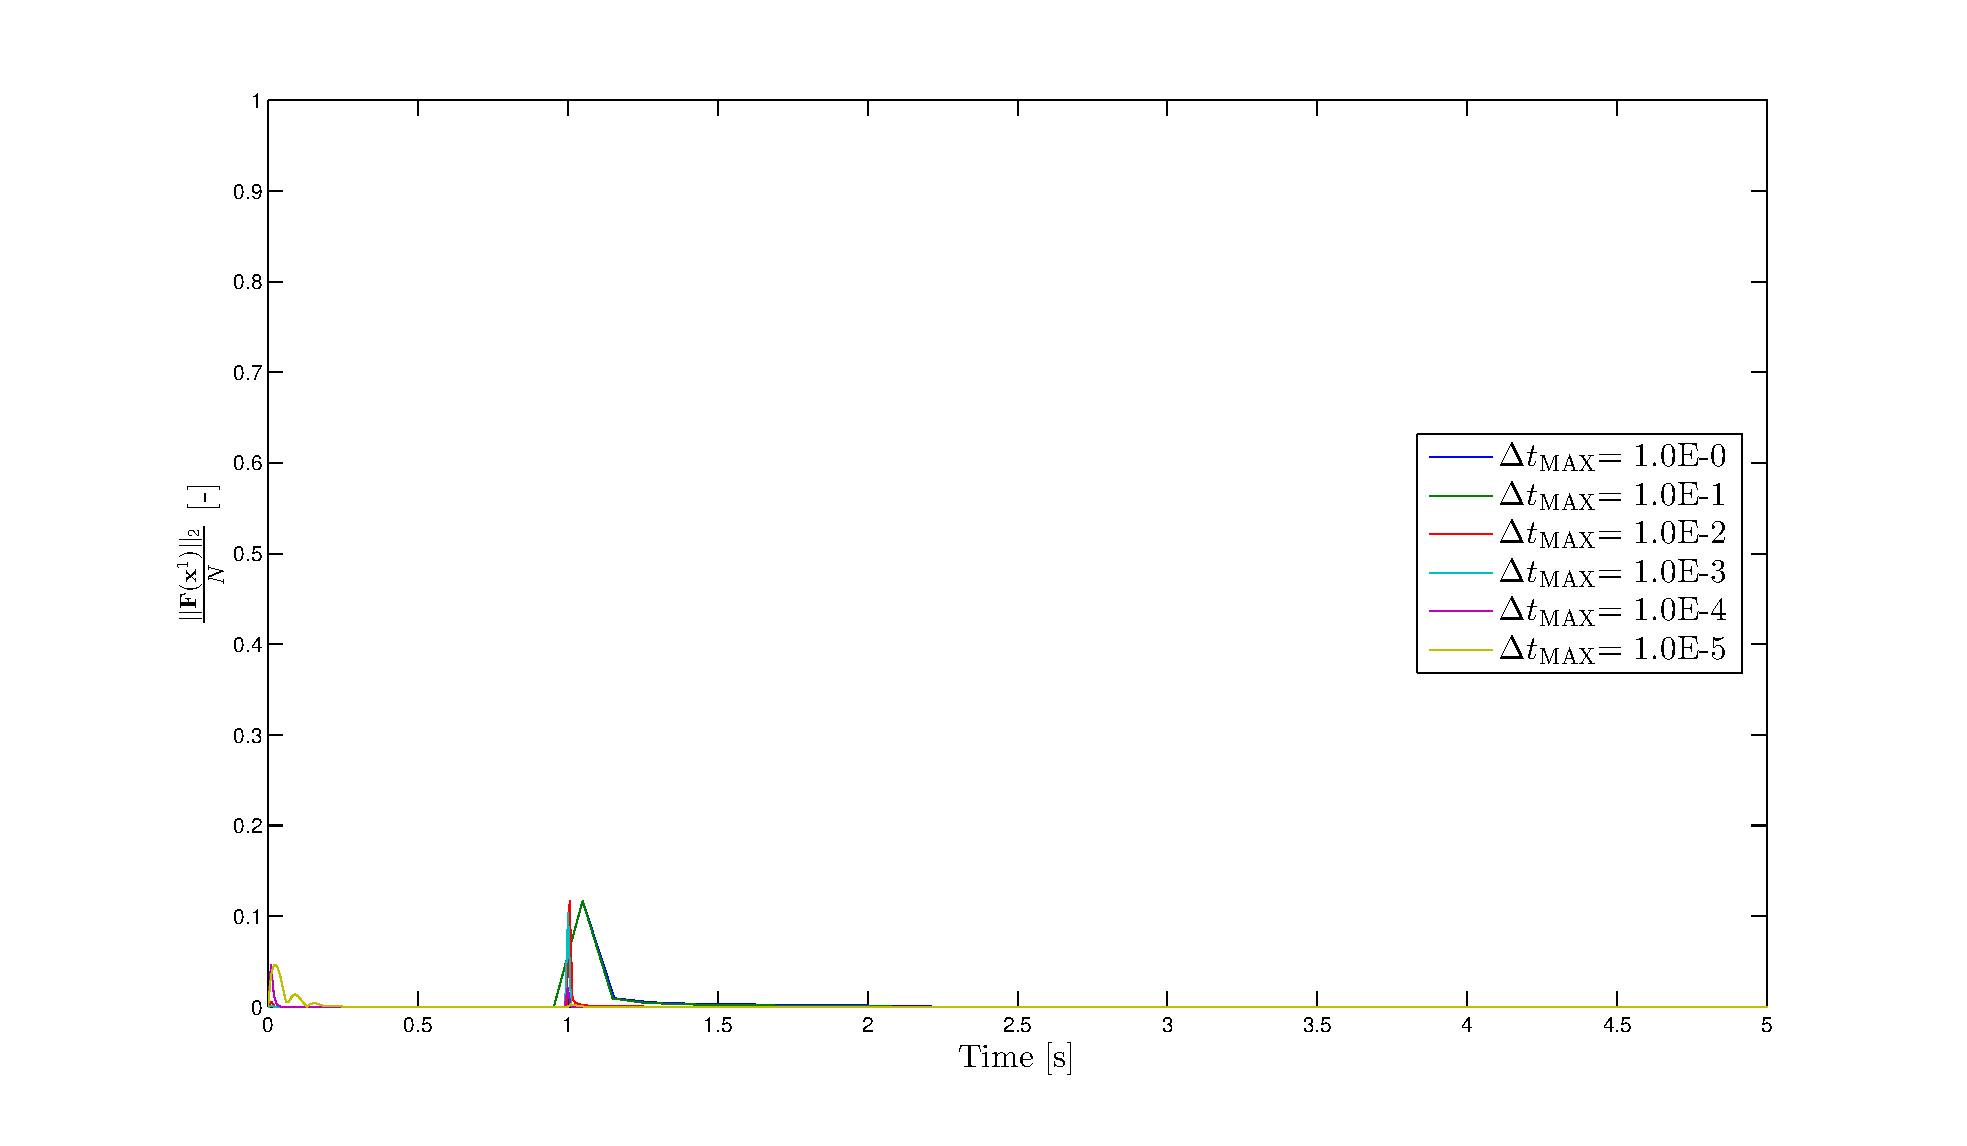
\includegraphics[width=0.49\textwidth]{images/cobra_single_res_v_dt.eps}
%\label{fig:leg_single_res}}
%\subfloat[Nonlinear mode.]{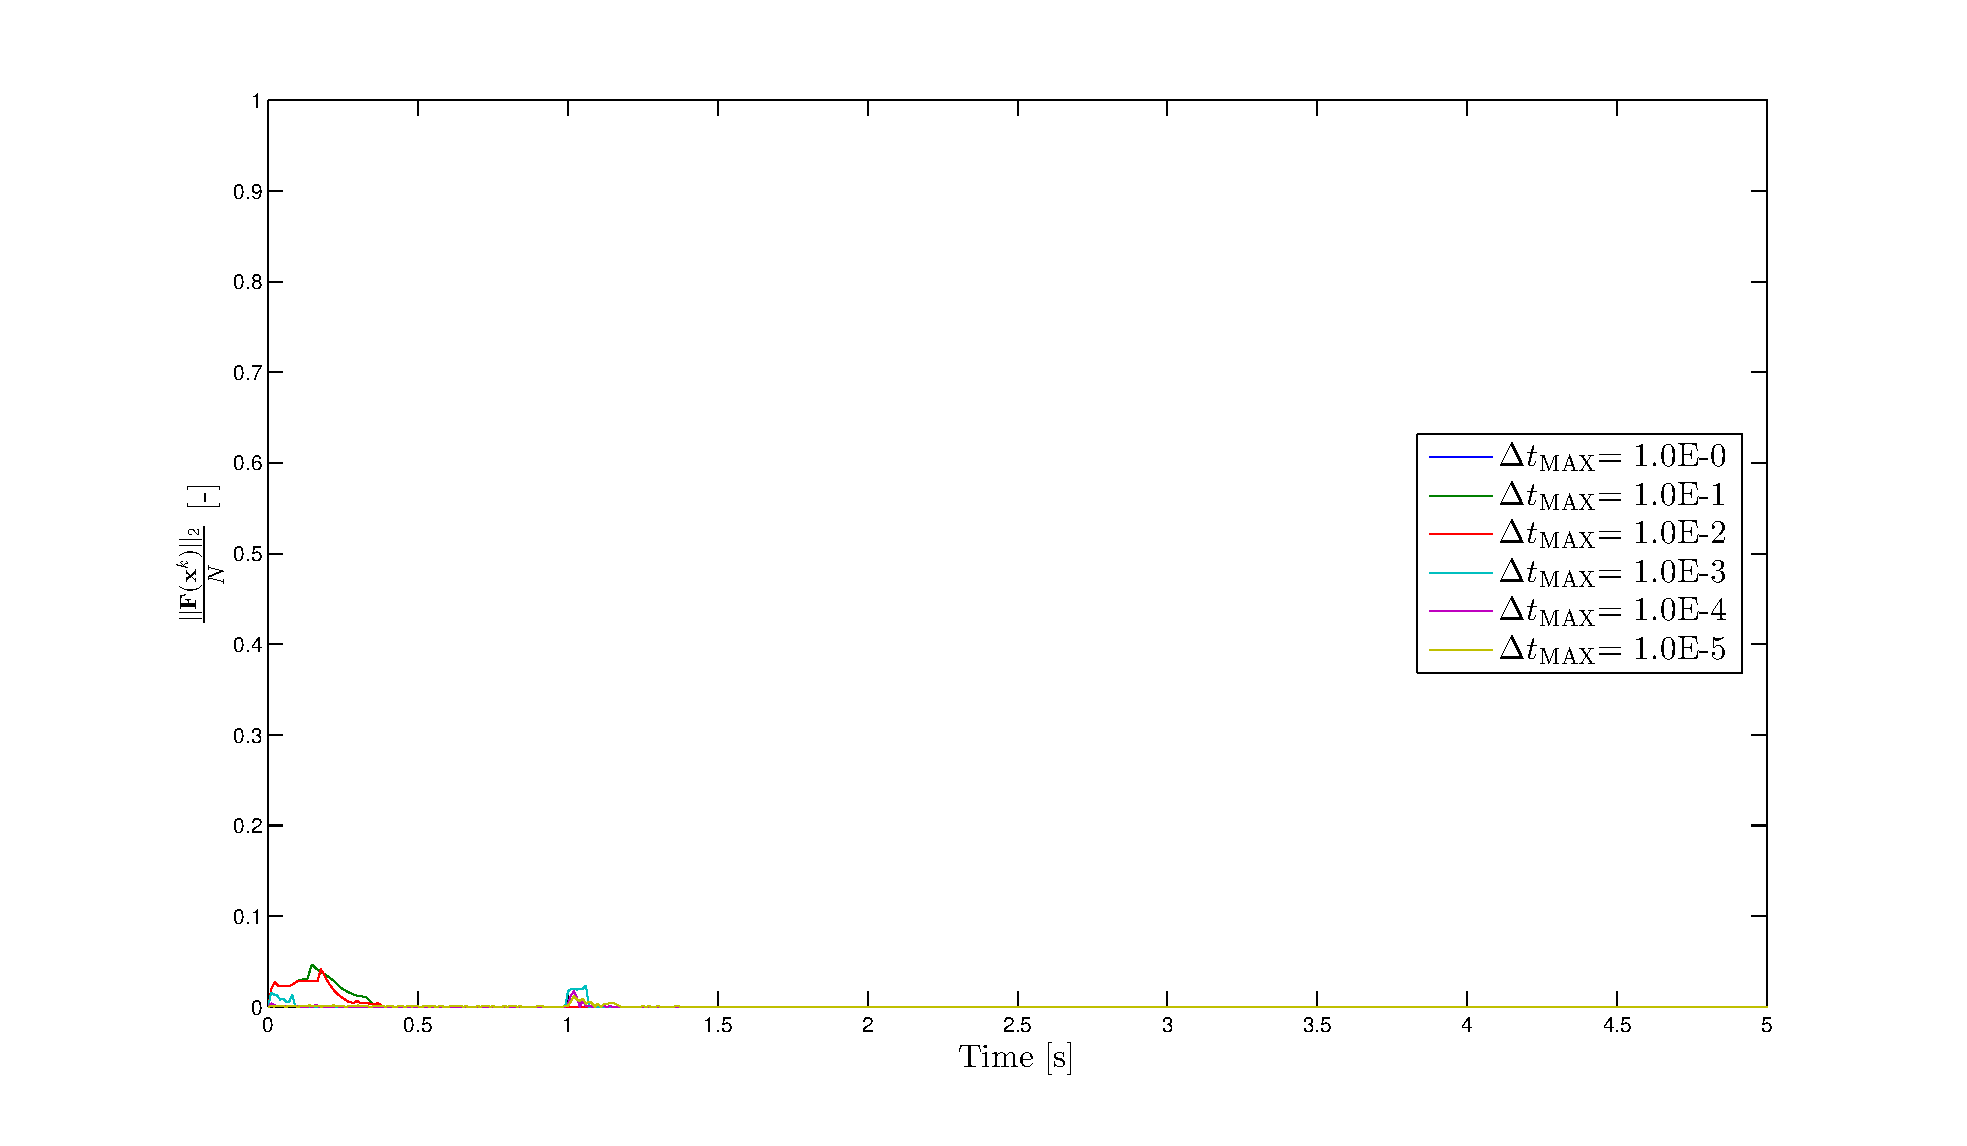
\includegraphics[width=0.49\textwidth]{images/nl_single_res_v_dt.eps}
%\label{fig:nl_single_res}}
%\caption[Single-phase residuals.]{Single-phase residuals.}
%\label{fig:single_compare_2}
%\end{figure}

\begin{figure}[h!t]
\centering
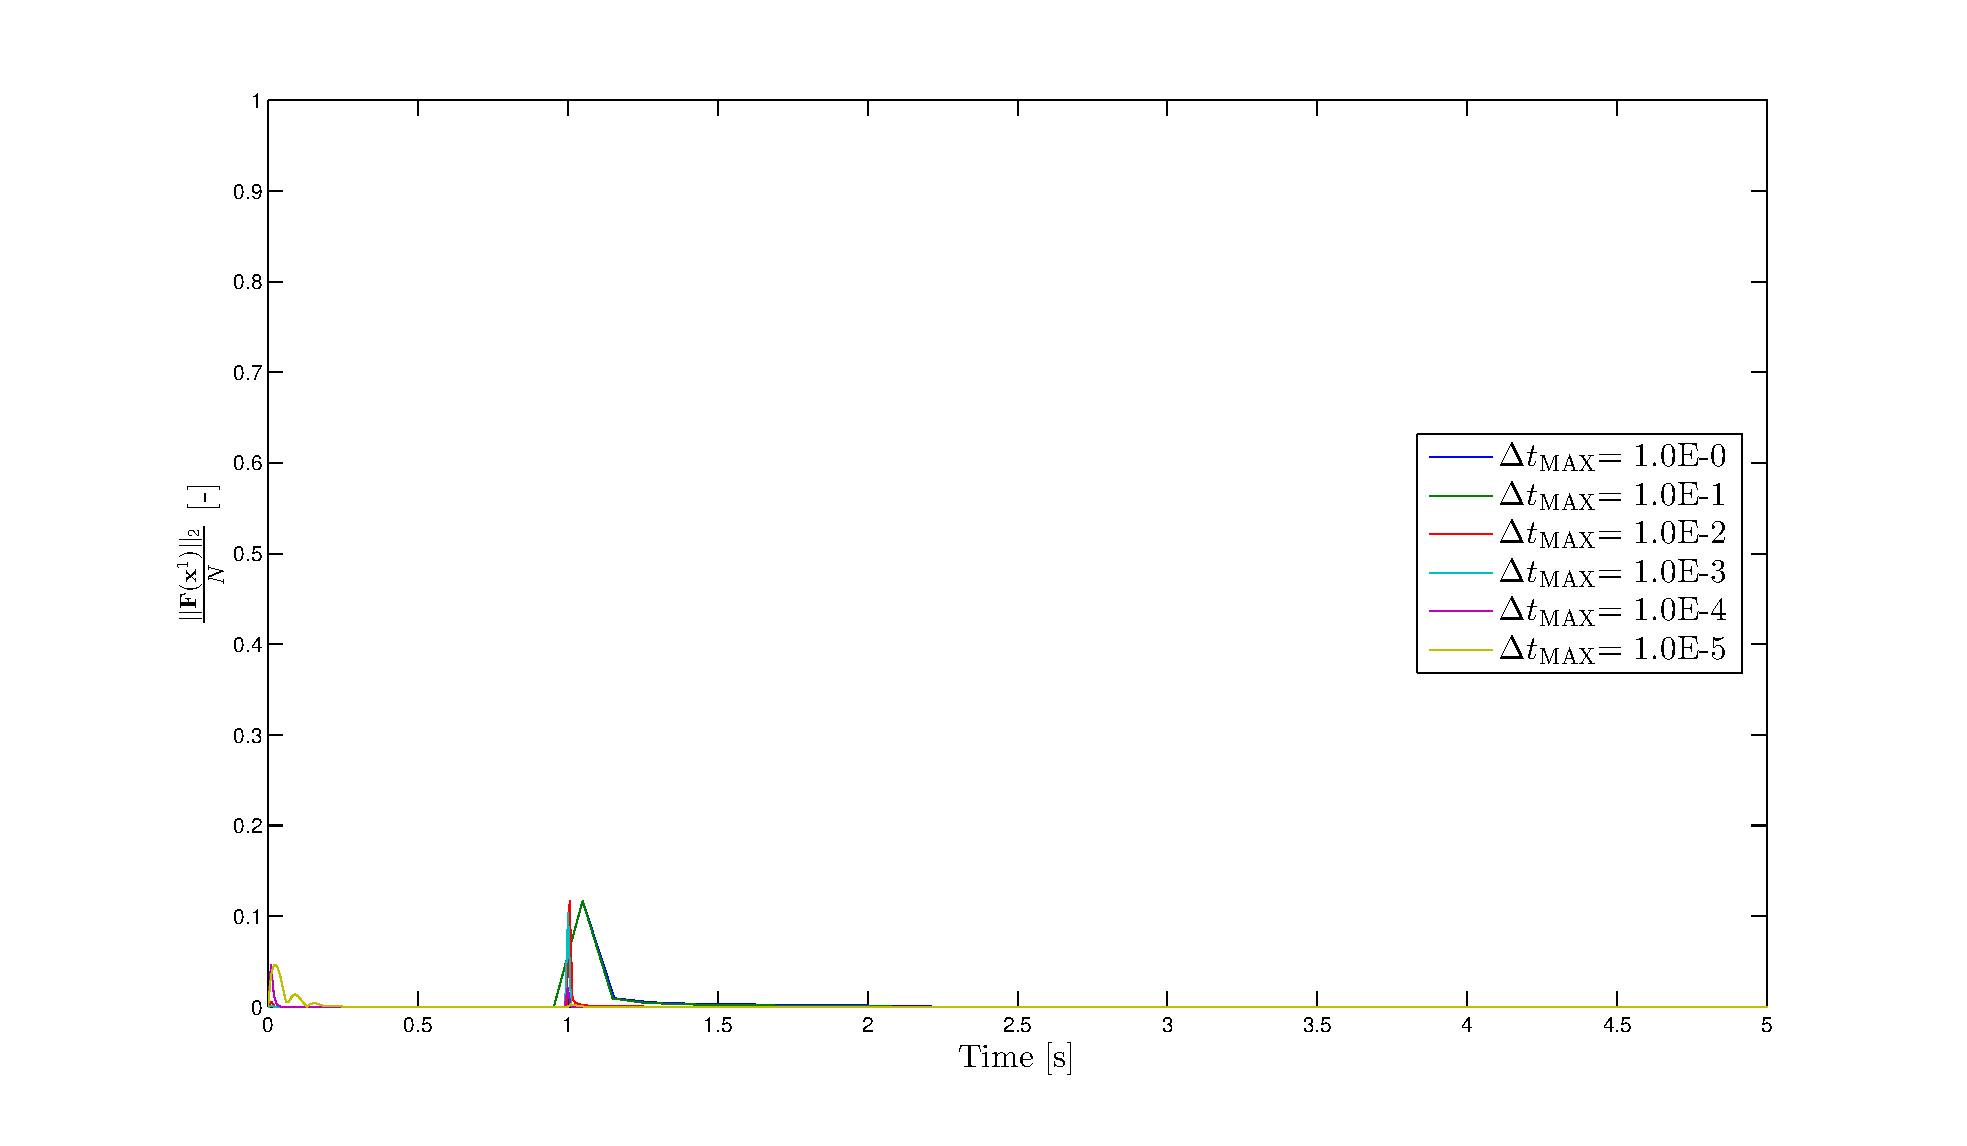
\includegraphics[width=0.94\textwidth]{images/cobra_single_res_v_dt.eps}
\caption{Legacy solver single-phase residuals.}
\label{fig:leg_single_res}
\end{figure}

\begin{figure}[h!t]
\centering
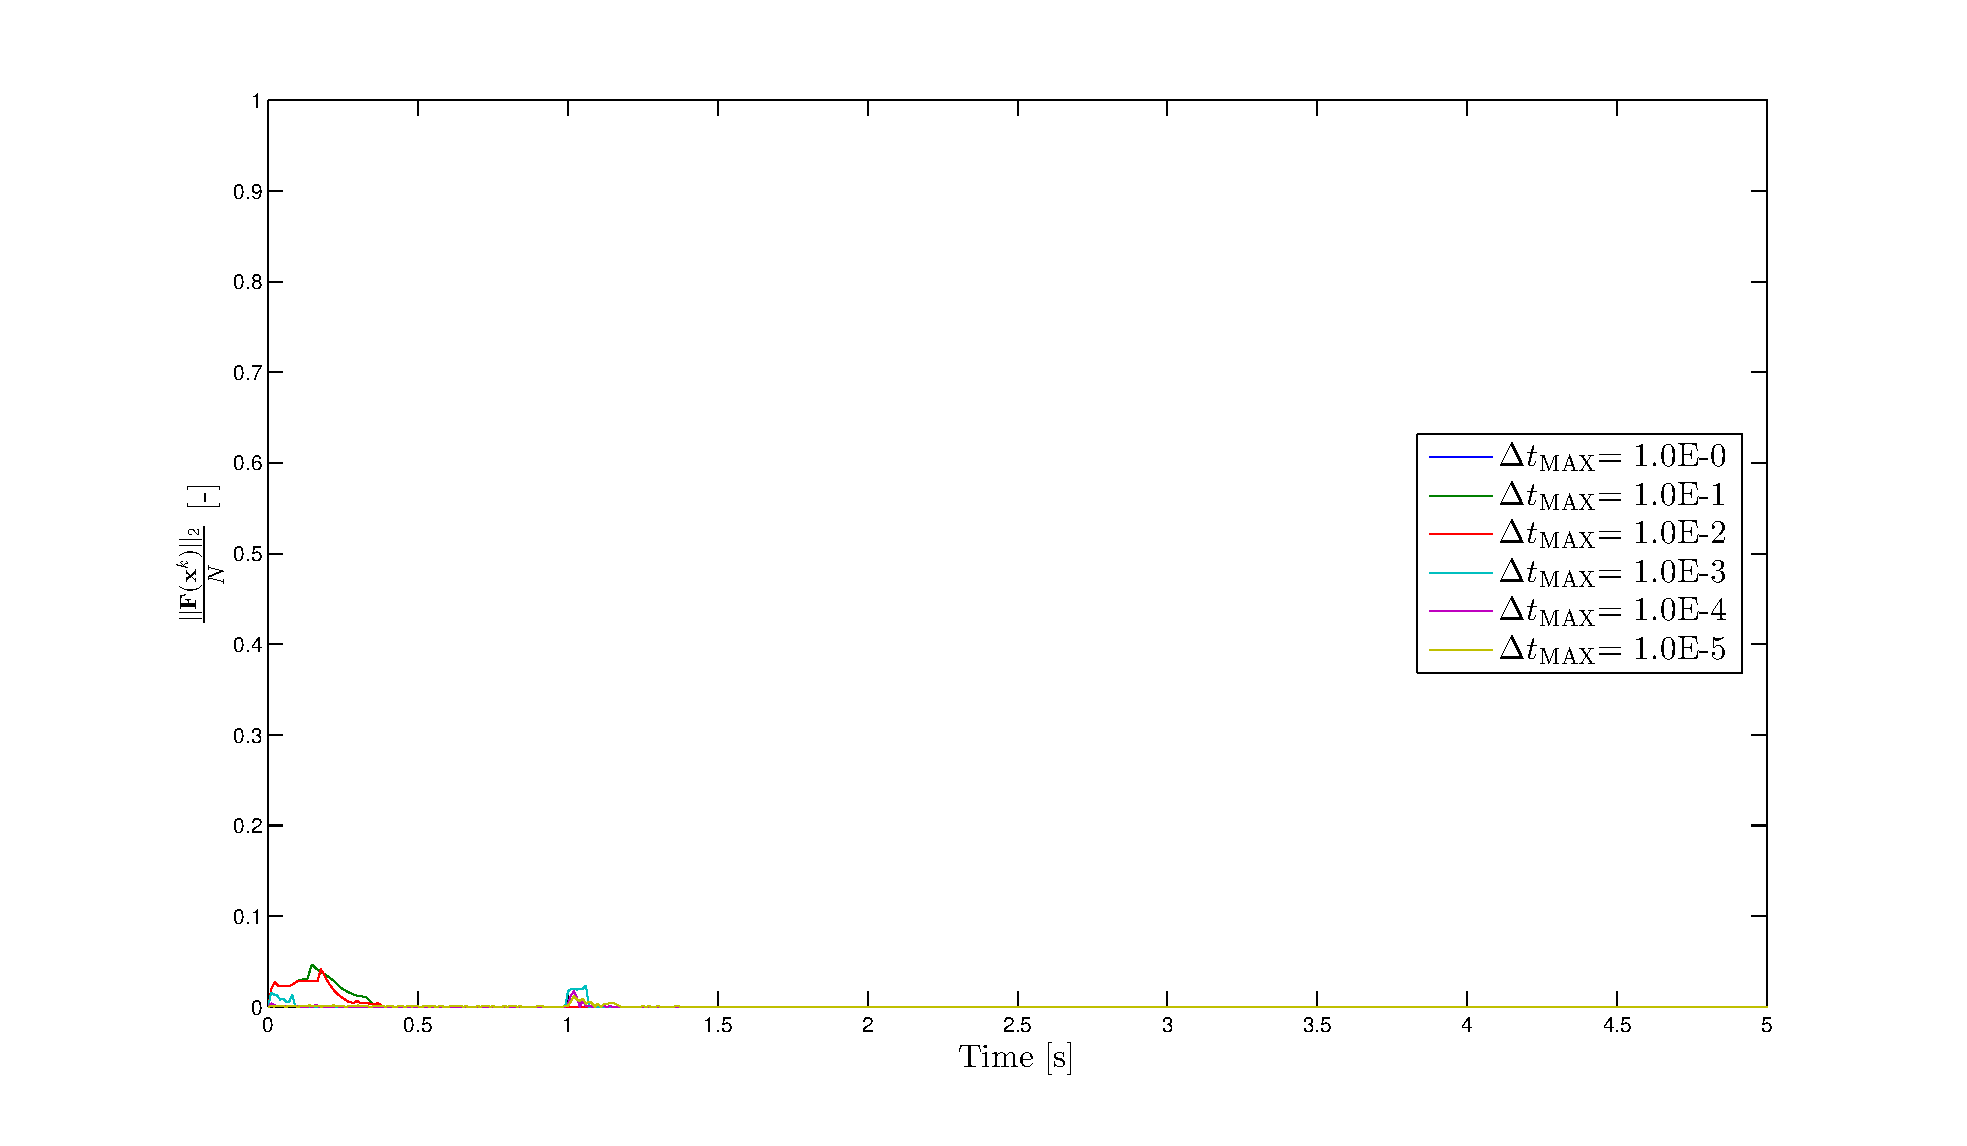
\includegraphics[width=0.94\textwidth]{images/nl_single_res_v_dt.eps}
\caption{Nonlinear solver single-phase residuals.}
\label{fig:nl_single_res}
\end{figure}

Examining the residual for the two different solvers will provide insight into how well each of them are at solving the nonlinear problem.
The residual of the legacy solver solution for the single-phase problem, \fig{fig:leg_single_res}, shows that the nonlinear residuals are nontrivial during two periods of the transient.
The first region of nontrivial residuals is present only for larger values of \dtmax{} and occurs when the the inlet flow initiates at 1 [s].
The second region occurs at smaller values of \dtmax{} and occurs near the beginning of the transient.
For the nonlinear solver solution residuals, \fig{fig:nl_single_res}, the same two regions, the start of simulation and the inlet flow initialization, exhibit similar nontrivial residuals.
However, the behavior of the residual for the nonlinear solver as a function of \dtmax{} exhibits an anomaly that is absent in the legacy solver.
To put the anomaly in context it should first be noted that the nonlinear residual at the initiation of the ramp is approximately zero for \dtmax{} = 1 [s] and \dtmax{} = 1.0E-5 [s].
It is only during intermediate values of \dtmax{} that the residuals becomes nontrivial during the ramp initiation.

%\begin{figure}[h!t]
%\centering
%\subfloat[Transient Solution]{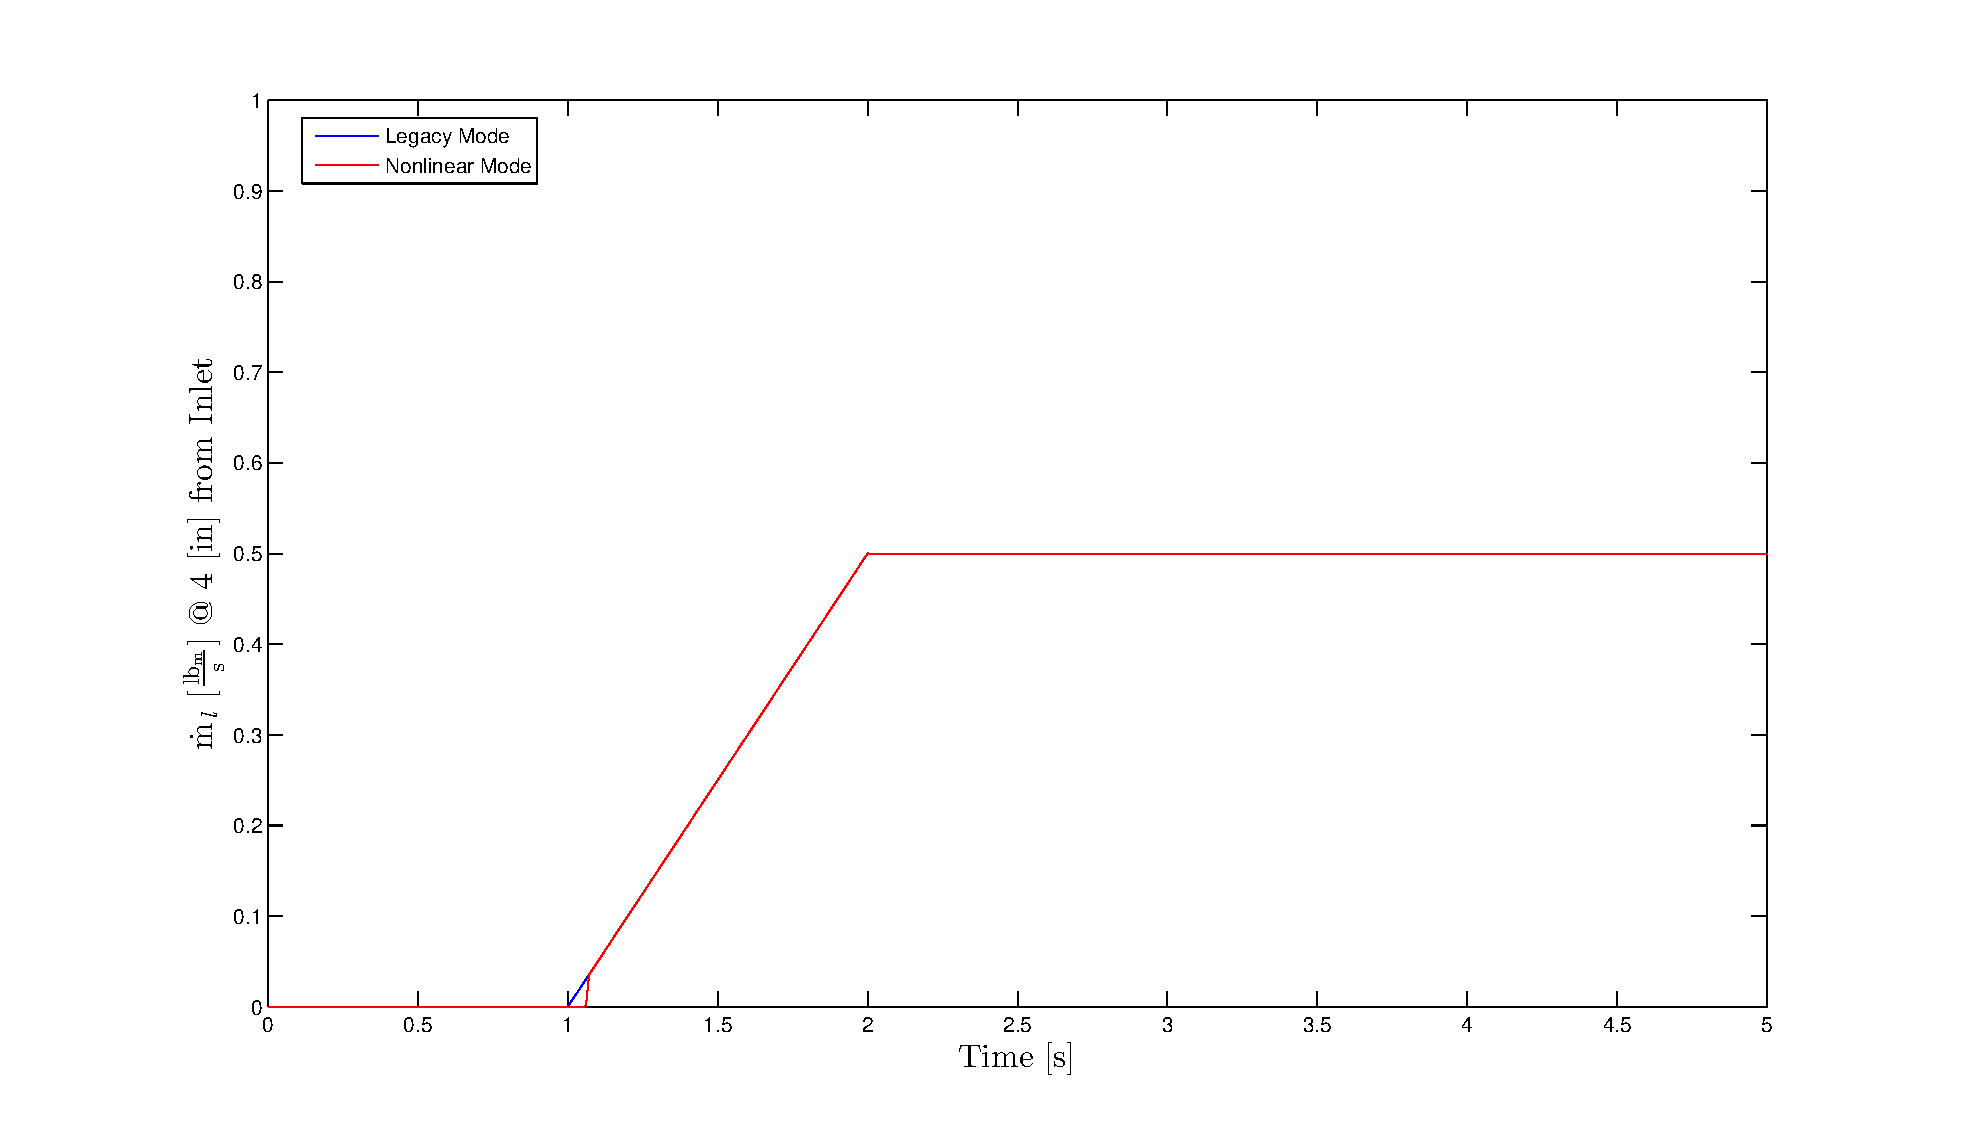
\includegraphics[width=0.49\textwidth]{images/single_1em3.eps}
%\label{fig:single_1em3}}
%\subfloat[Zoomed Solution]{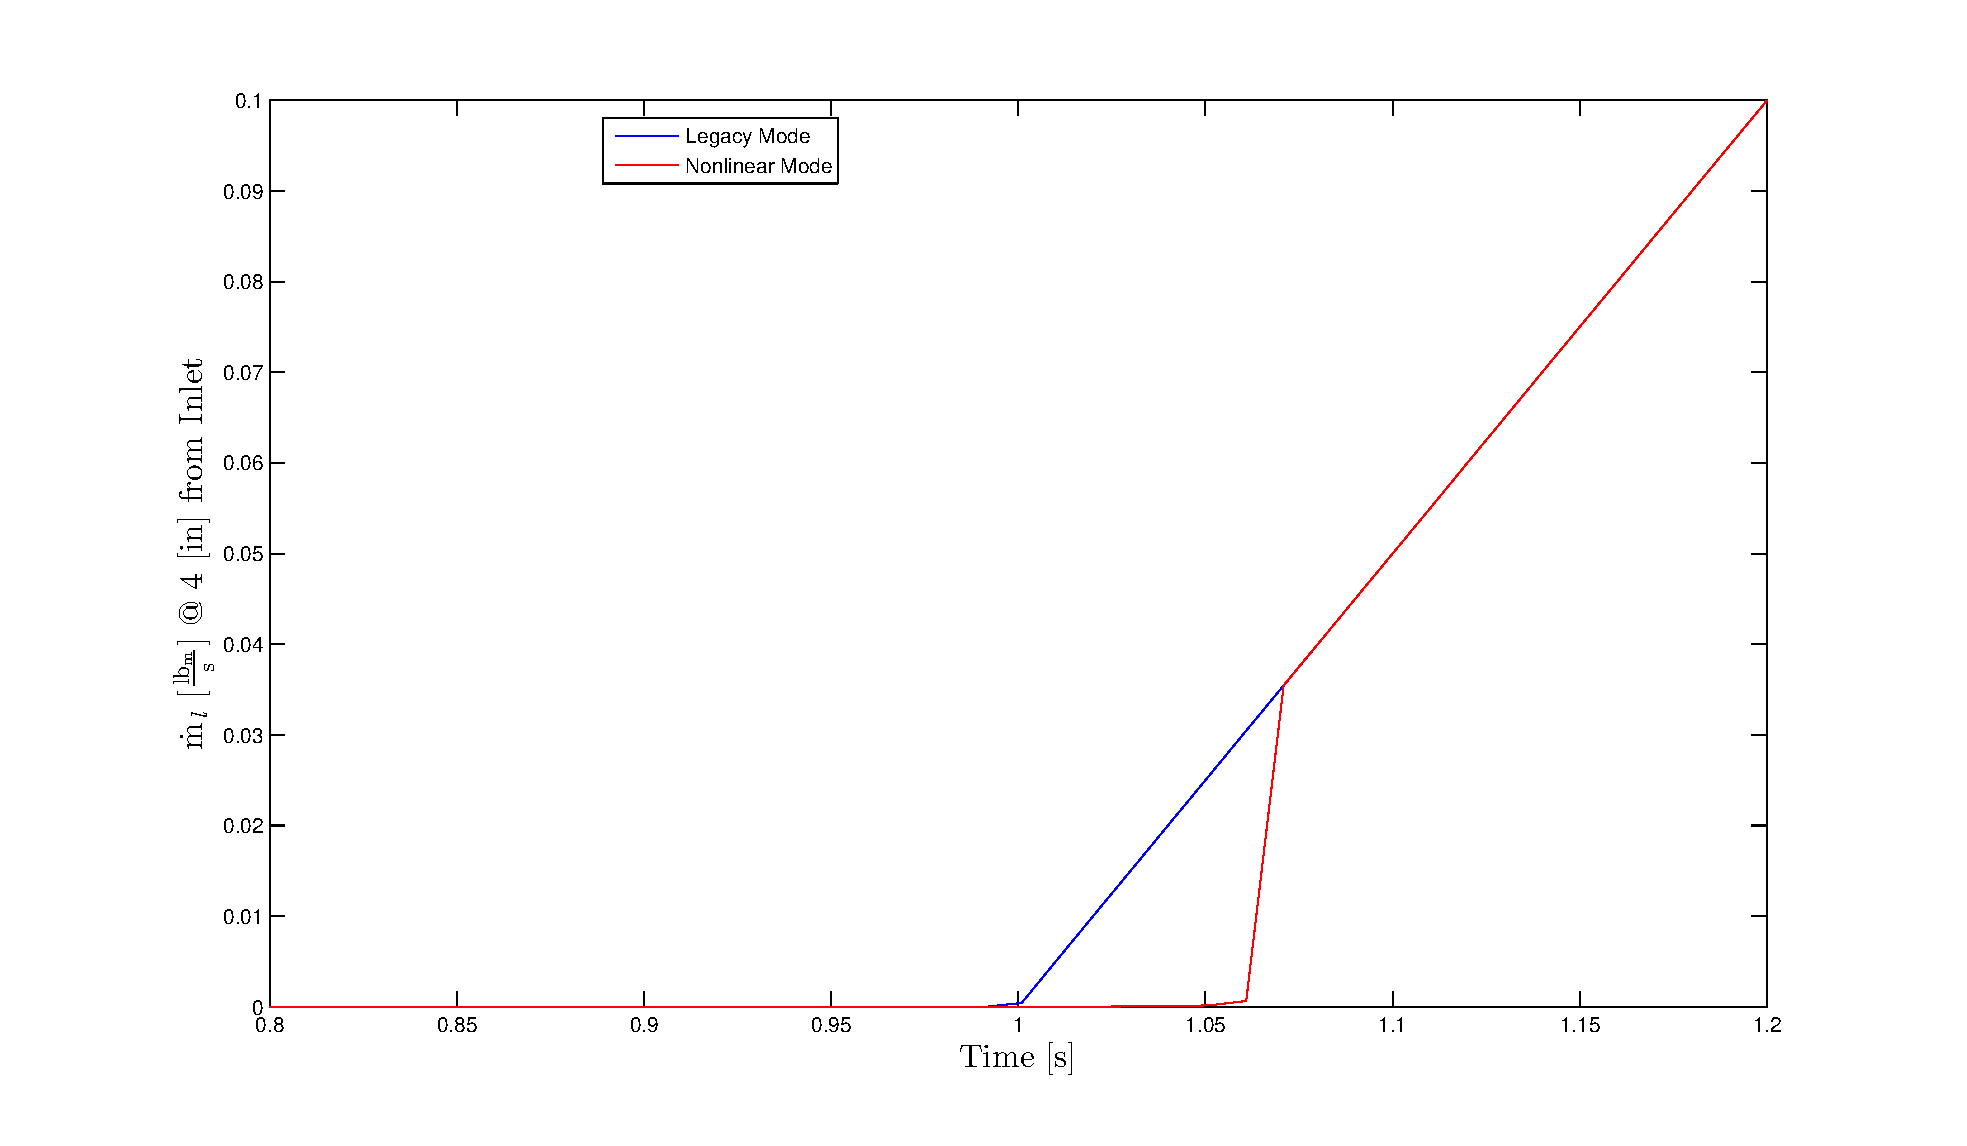
\includegraphics[width=0.49\textwidth]{images/single_1em3_zoom.eps}
%\label{fig:single_1em3_zoom}}
%\caption[Single-phase solution at \dtmax{} = 1.0E-3 {[s]}]{Single-phase solution with \dtmax{} = 1.0E-3 {[s]}.}
%\label{fig:single_compare_3}
%\end{figure}

\begin{figure}[h!t]
\centering
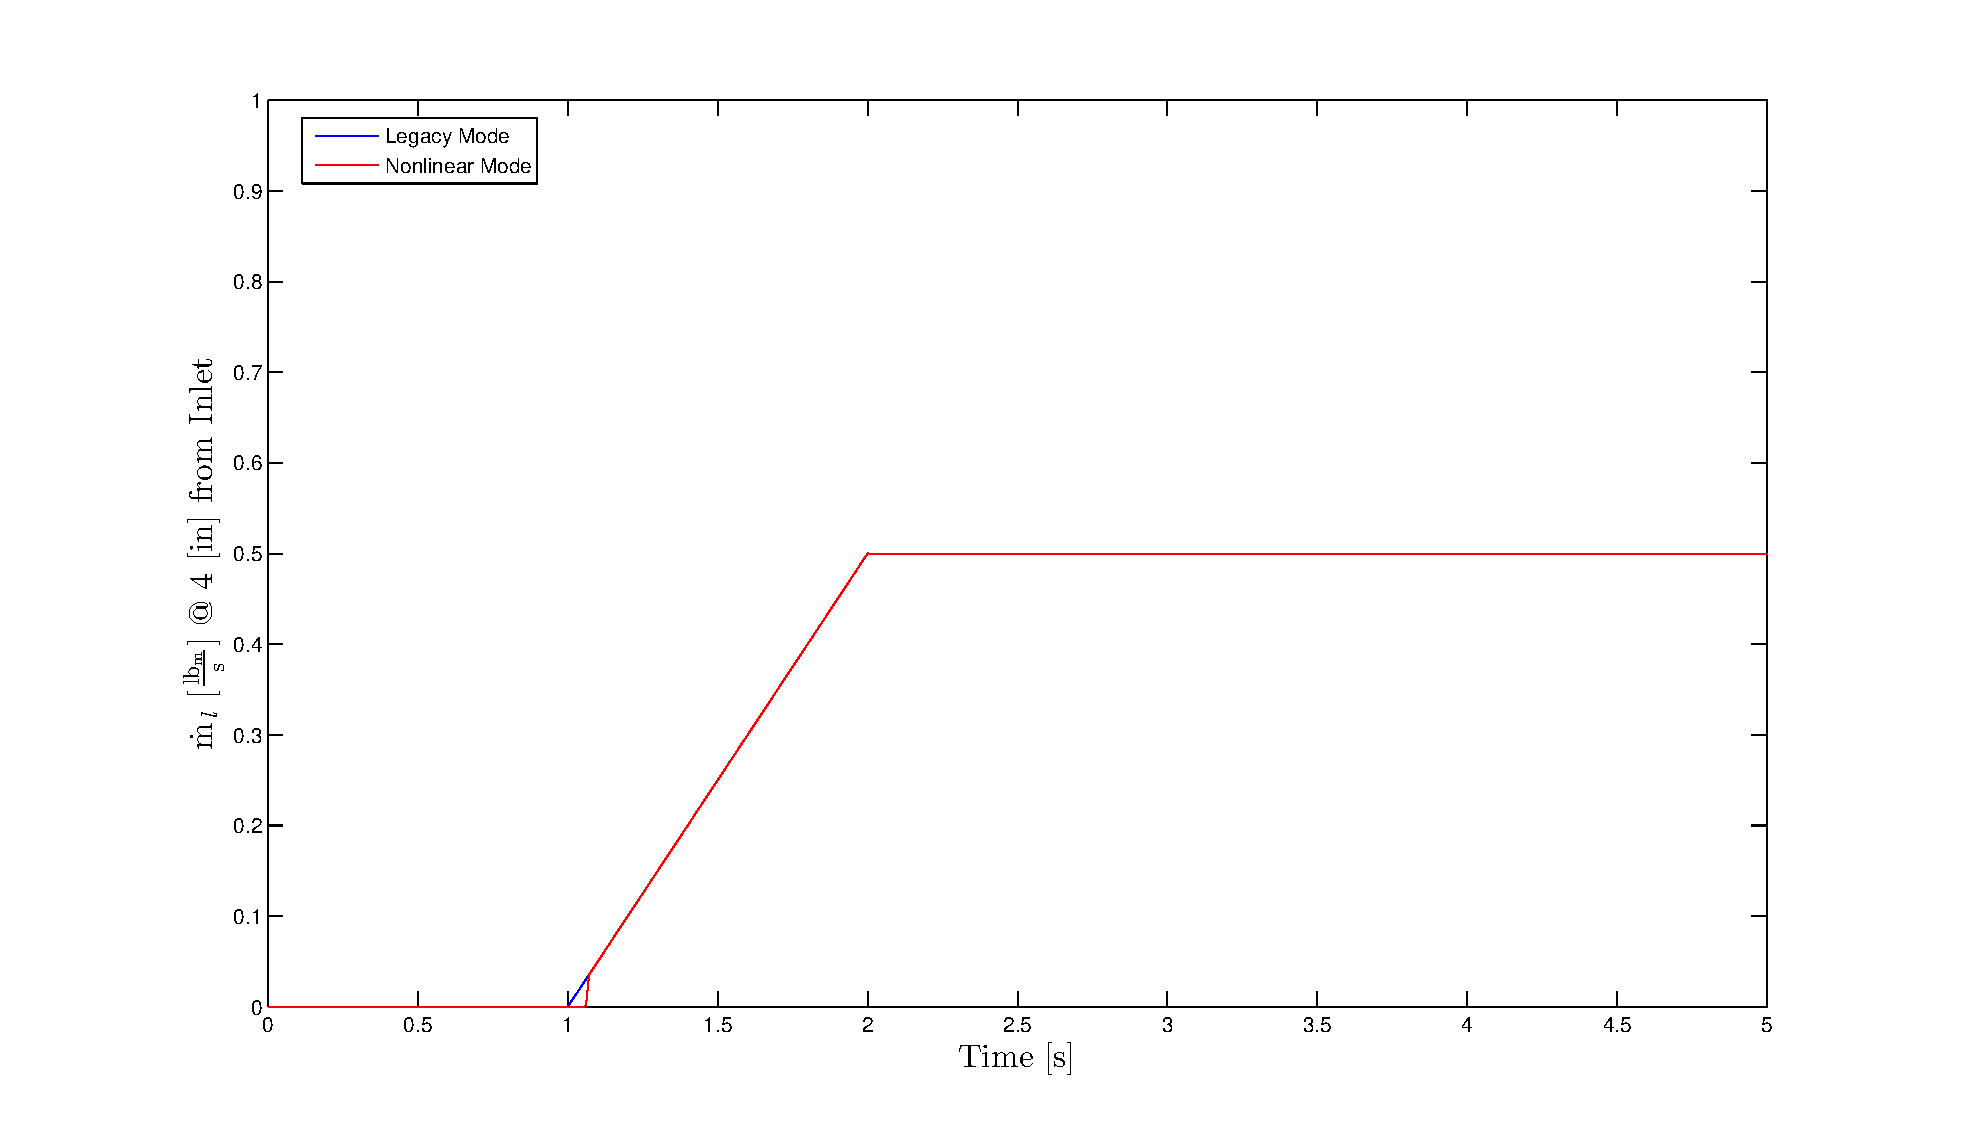
\includegraphics[width=0.94\textwidth]{images/single_1em3.eps}
\caption{Full transient single-phase solution with \dtmax{} = 1.0E-3 {[s]}.}
\label{fig:single_1em3}
\end{figure}

\begin{figure}[h!t]
\centering
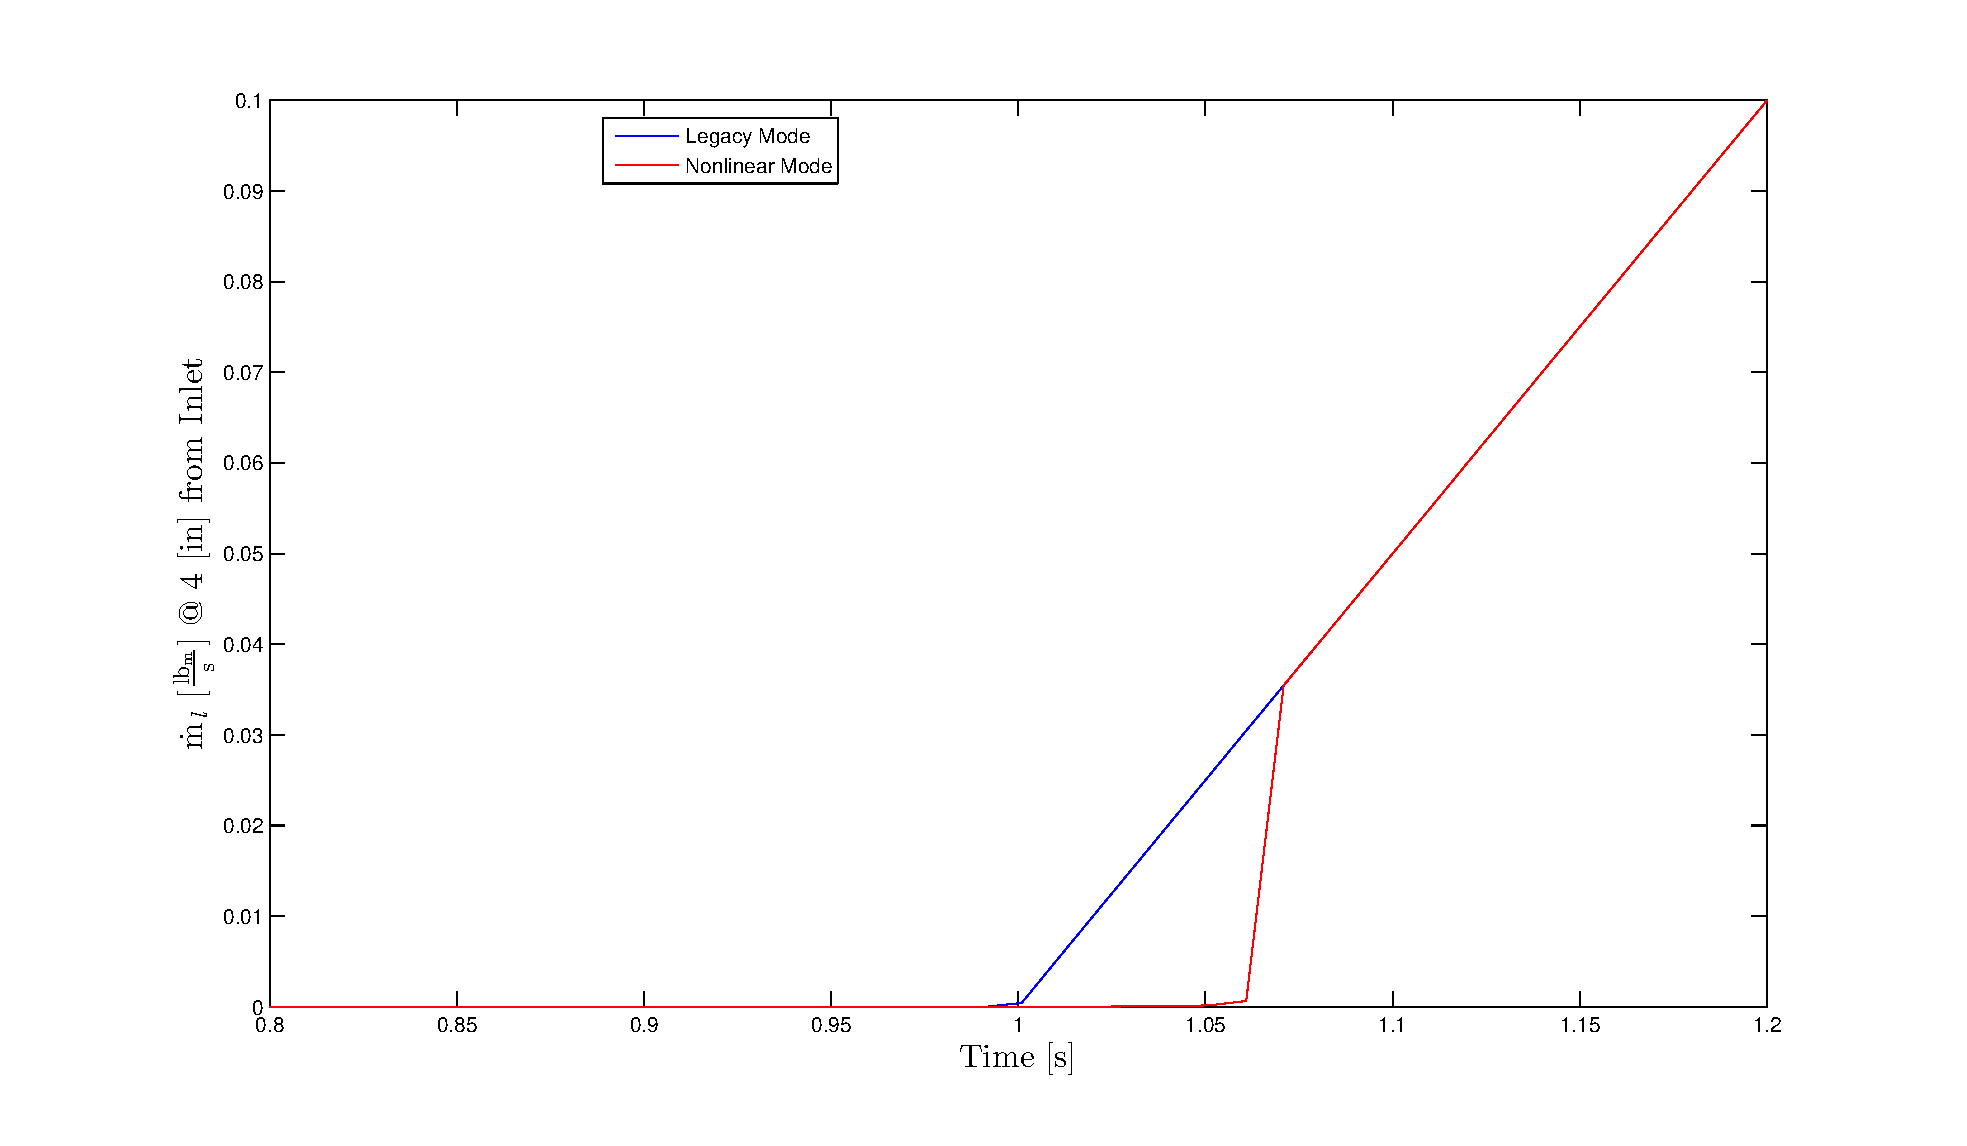
\includegraphics[width=0.94\textwidth]{images/single_1em3_zoom.eps}
\caption{Zoomed single-phase solution with \dtmax{} = 1.0E-3 {[s]}.}
\label{fig:single_1em3_zoom}
\end{figure}

While the solutions at \dtmax{} = 1.0 [s] and \dtmax{} = 1.0E-5 [s] are identical for the two solver modes, the solutions at intermediate timestep sizes were not identical.
In particular, the nonlinear solver produces a solution at \dtmax{} = 1.0E-3 [s] that is inconsistent with both the solution produced by the legacy solver and, more importantly, with the specified inlet boundary conditions.
The two solvers produce solutions that agree for most of the domain, \fig{fig:single_1em3}, except at the initiation of the inlet flow at 1 [s], \fig{fig:single_1em3_zoom}.

%\begin{figure}[h!t]
%\centering
%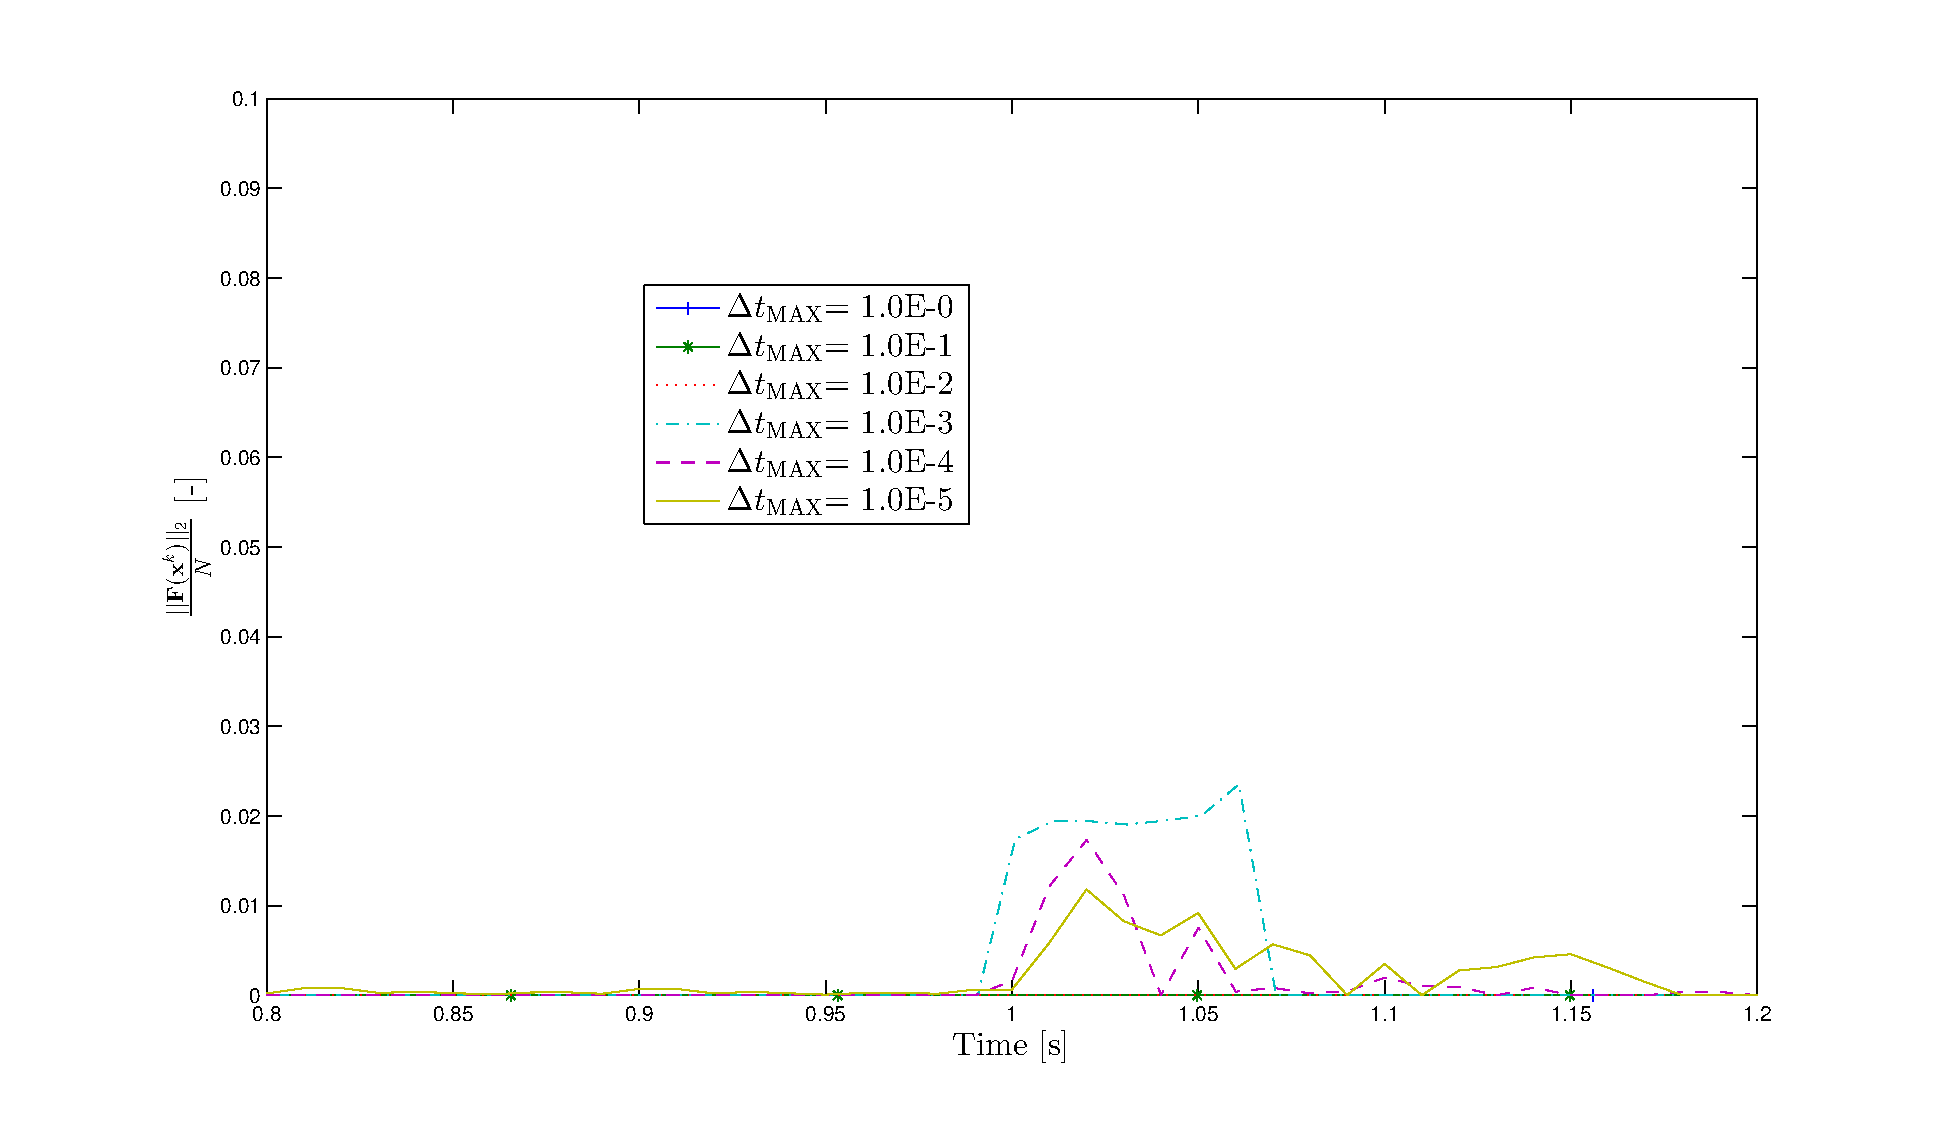
\includegraphics[width=0.49\textwidth]{images/nl_res_single_zoom.eps}
%\caption{Nonlinear mode solution residual for single-phase problem.}
%\label{fig:nl_res_single_zoom}
%\end{figure}

\begin{figure}[h!t]
\centering
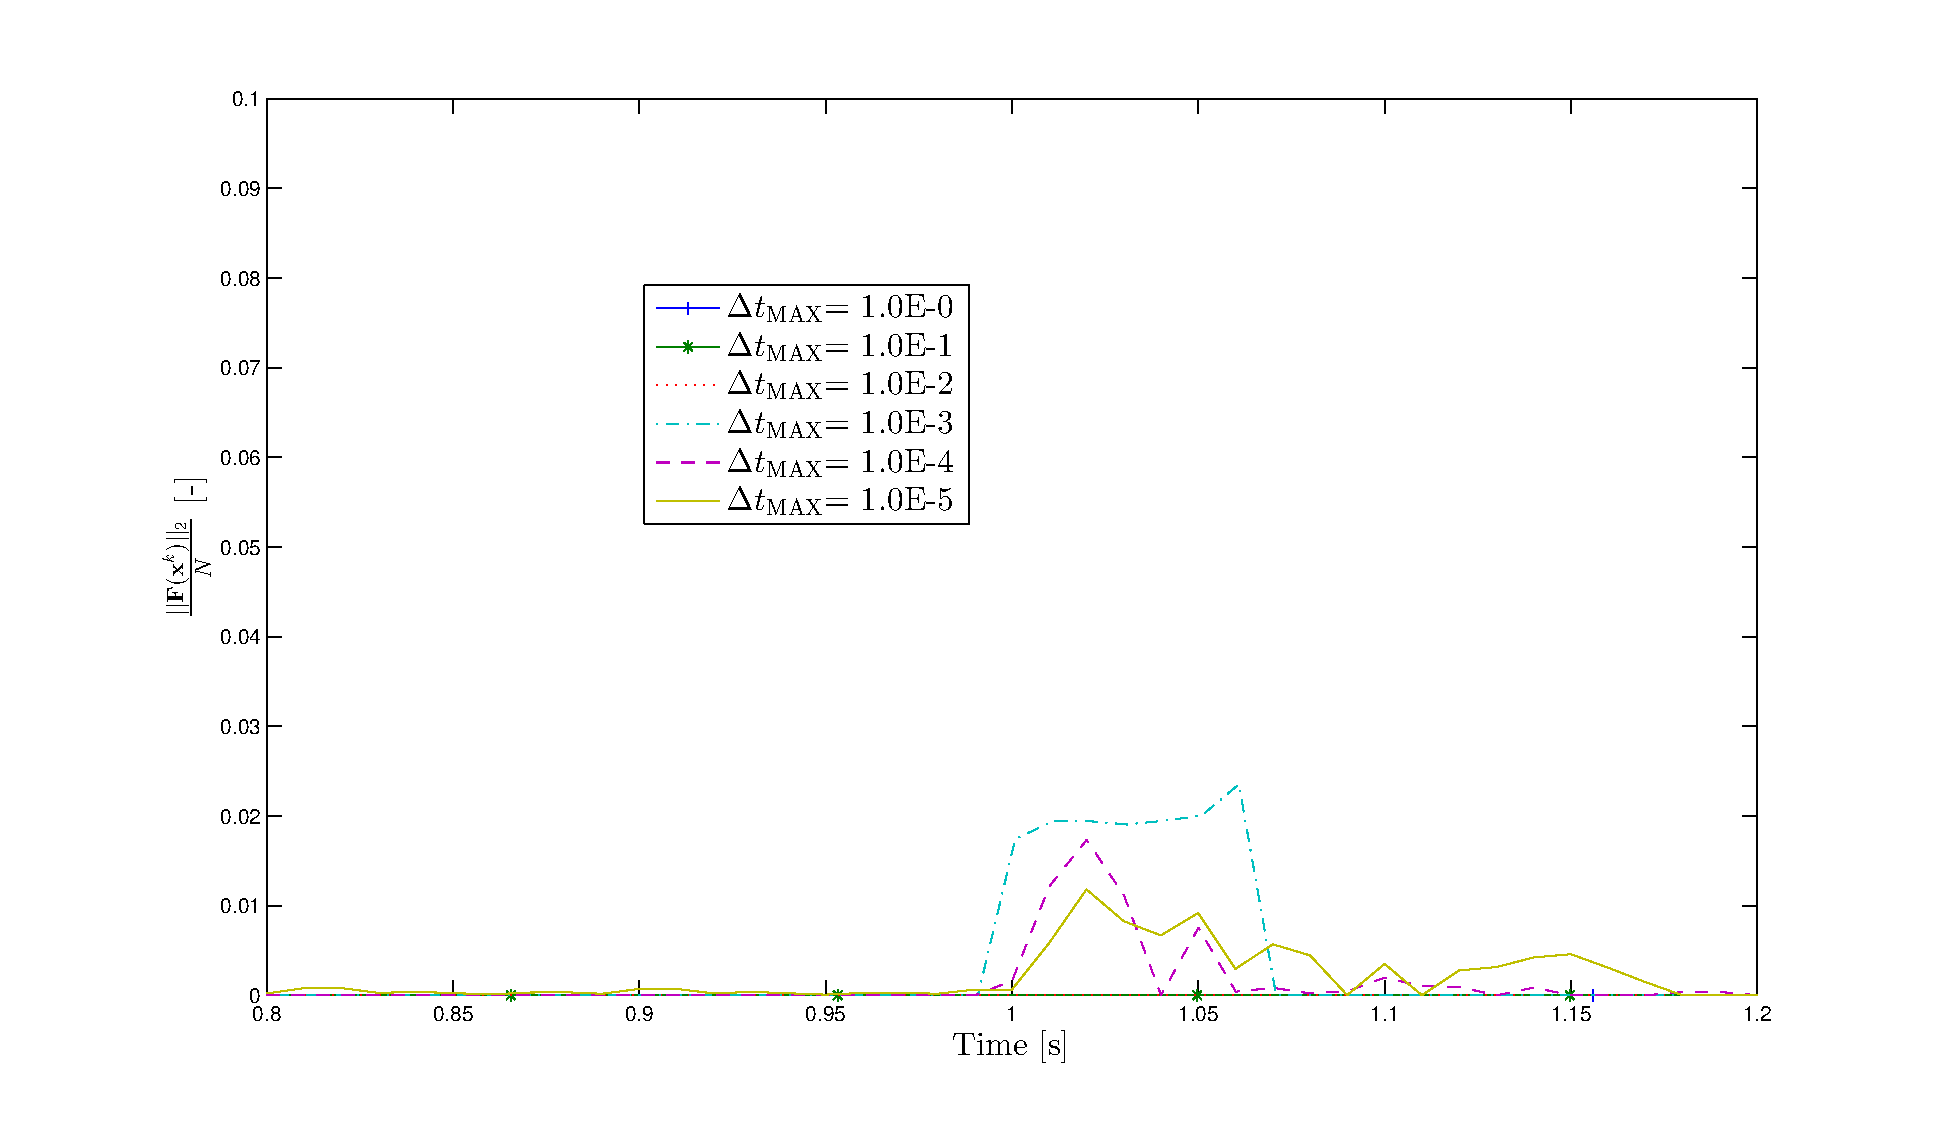
\includegraphics[width=0.94\textwidth]{images/nl_res_single_zoom.eps}
\caption{Zoomed residuals for the single-phase solution from the nonlinear solver.}
\label{fig:nl_res_single_zoom}
\end{figure}

This difference is manifested in the residuals for the nonlinear solver solution around 1 [s], \fig{fig:nl_res_single_zoom}.
The residual at the time of inlet flow initialization has a marked increase between the \dtmax{} = 1.0E-3 and \dtmax{} = 1.0E-2 solutions.
The reason for this behavior is, as of yet, unknown.
It is likely related to the same nonlinear non-convergence behavior remarked upon for the flashing problem. 

One way to quantify the difference between the solutions is by measuring the residual convergence metrics outlined in \sect{sect:temporal_convergence}.
These metrics provide a measure of how poorly the discrete nonlinear equations are being solved at every timestep in the transient.
The resolution of the residual allows for a solution that is less sensitive to timestep size selection than for a solution that does not resolve the residual.
The convergence metrics will be used to determine if a qualitative temporal-convergence determination can lead to the acceptance of a solution that is not nonlinearly converged.

For each of the test cases, the two different metrics were compared at the different \dtmax{}.
To examine efficacy of the the temporal convergence criteria, both the average and moment based temporal convergence criteria were evaluated for each of the twenty-three successful simulations.
The values of these metrics will be compared between different solvers for the same test problem. 

The two different nonlinear convergence metrics will now be examined for the flashing problem.
\tab{tab:flashing_criteria} shows both the average metric, $\tilde{R}$, and the moment based metric, $\tilde{R}_{\text{M}}$.
The entry for the legacy mode solution at 1 [s] is empty, reflecting its inability to solve the problem.
For the nonlinear solver, both metrics are decreasing as the \dtmax{} is decreased.
While the legacy solver also shows a decreasing residual metric, it does not decrease in order-of-magnitude, indicating that as the \dtmax{} is reduced the nonlinearities in the problem are not being sufficiently resolved.

\begin{table}[h!t]
\centering
\begin{tabular}{@{}l r@{.}l r@{.}l r@{.}l r@{.}l @{}}
\toprule
& \multicolumn{4}{c}{$\tilde{R}$} & \multicolumn{4}{c}{$\tilde{R}_{\text{M}}$}  \\
$\dtmax{}$ & \multicolumn{2}{c}{Legacy} & \multicolumn{2}{c}{Nonlinear} & \multicolumn{2}{c}{Legacy}& \multicolumn{2}{c}{Nonlinear}  \\
\midrule
1.0    & \multicolumn{2}{c}{-} & 1&177E-3 & \multicolumn{2}{c}{-} & 6&885E-4 \\
1.0E-1 & 5&487E-2 & 1&141E-3 & 5&044E-2 & 6&730E-4 \\
1.0E-2 & 4&960E-2 & 3&413E-4 & 4&570E-2 & 2&511E-4 \\
1.0E-3 & 3&172E-2 & 2&669E-4 & 2&372E-2 & 1&975E-4 \\
1.0E-4 & 2&504E-2 & 1&346E-4 & 1&838E-2 & 8&974E-5 \\
1.0E-5 & 2&166E-2 & 5&075E-5 & 1&922E-2 & 4&581E-5 \\
\bottomrule  
\end{tabular}
\caption{Nonlinear convergence metrics for flashing problem.}
\label{tab:flashing_criteria}
\end{table}

\begin{table}[h!t]
\centering
\begin{tabular}{@{}l r@{.}l r@{.}l r@{.}l r@{.}l @{}}
\toprule
& \multicolumn{4}{c}{$\tilde{R}$} & \multicolumn{4}{c}{$\tilde{R}_{\text{M}}$}  \\
$\dtmax{}$ & \multicolumn{2}{c}{Legacy} & \multicolumn{2}{c}{Nonlinear} & \multicolumn{2}{c}{Legacy}& \multicolumn{2}{c}{Nonlinear}  \\
\midrule
1.0    & 3&149E-3 & 1&700E-3 & 1&485E-3 & 1&070E-4 \\
1.0E-1 & 2&866E-3 & 1&700E-3 & 1&287E-3 & 1&070E-4 \\
1.0E-2 & 3&412E-4 & 1&357E-3 & 1&417E-4 & 7&701E-5 \\
1.0E-3 & 2&207E-4 & 4&584E-4 & 8&805E-5 & 1&178E-4 \\
1.0E-4 & 1&672E-4 & 1&588E-3 & 1&834E-5 & 4&958E-5 \\
1.0E-5 & 5&493E-4 & 2&758E-4 & 1&916E-5 & 8&939E-5 \\
\bottomrule  
\end{tabular}
\caption{Nonlinear convergence metrics for the single-phase problem.}
\label{tab:single_criteria}
\end{table}

\tab{tab:single_criteria} shows the two metrics for the single-phase problem.
Since the single-phase problem is relatively linear, the legacy solver produces metrics that are on the same order as those for the nonlinear solver.
Due to the non-convergence of the nonlinear solver at \dtmax{} = 1.0E-3, the moment based metric for the nonlinear solver is greater than the equivalent legacy solver metric.

